% =====================================================================
%  Phụ lục: Mô hình chi tiết các phân hệ từ 5 tệp thiết kế Draw.io
%  Order&OrderHistory, Quản lý Sản phẩm, Quản lý Nguyên liệu, Cart, BrewLite
% =====================================================================
\clearpage
\appendix

% ---------------------------------------------------------------------
%  PHỤ LỤC A: THỰC ĐƠN VÀ DANH MỤC
% ---------------------------------------------------------------------
\section{Phân hệ Thực đơn và Danh mục (Menu \& Catalog Module)}
\label{app:menu}
Nguồn thiết kế: \file{BrewLite.drawio}. Phân hệ Thực đơn và Danh mục là điểm chạm đầu tiên của khách hàng với hệ thống BrewLite, cho phép duyệt danh sách đồ uống phân theo danh mục (Cà phê, Trà \& Trái cây, Đá xay), lọc nhanh và tìm kiếm món uống theo tên tiếng Việt không dấu.

\begin{figure}[H]
\centering
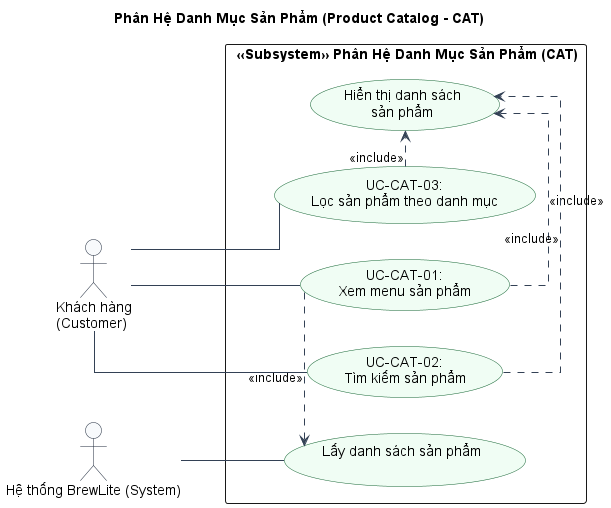
\includegraphics[width=0.82\textwidth,height=0.45\textheight,keepaspectratio]{../figures/diagrams/usecase-product-catalog.png}
\caption{Use Case Diagram: Phân hệ Thực đơn và Danh mục sản phẩm}
\label{fig:uc-menu}
\end{figure}

\begin{figure}[H]
\centering
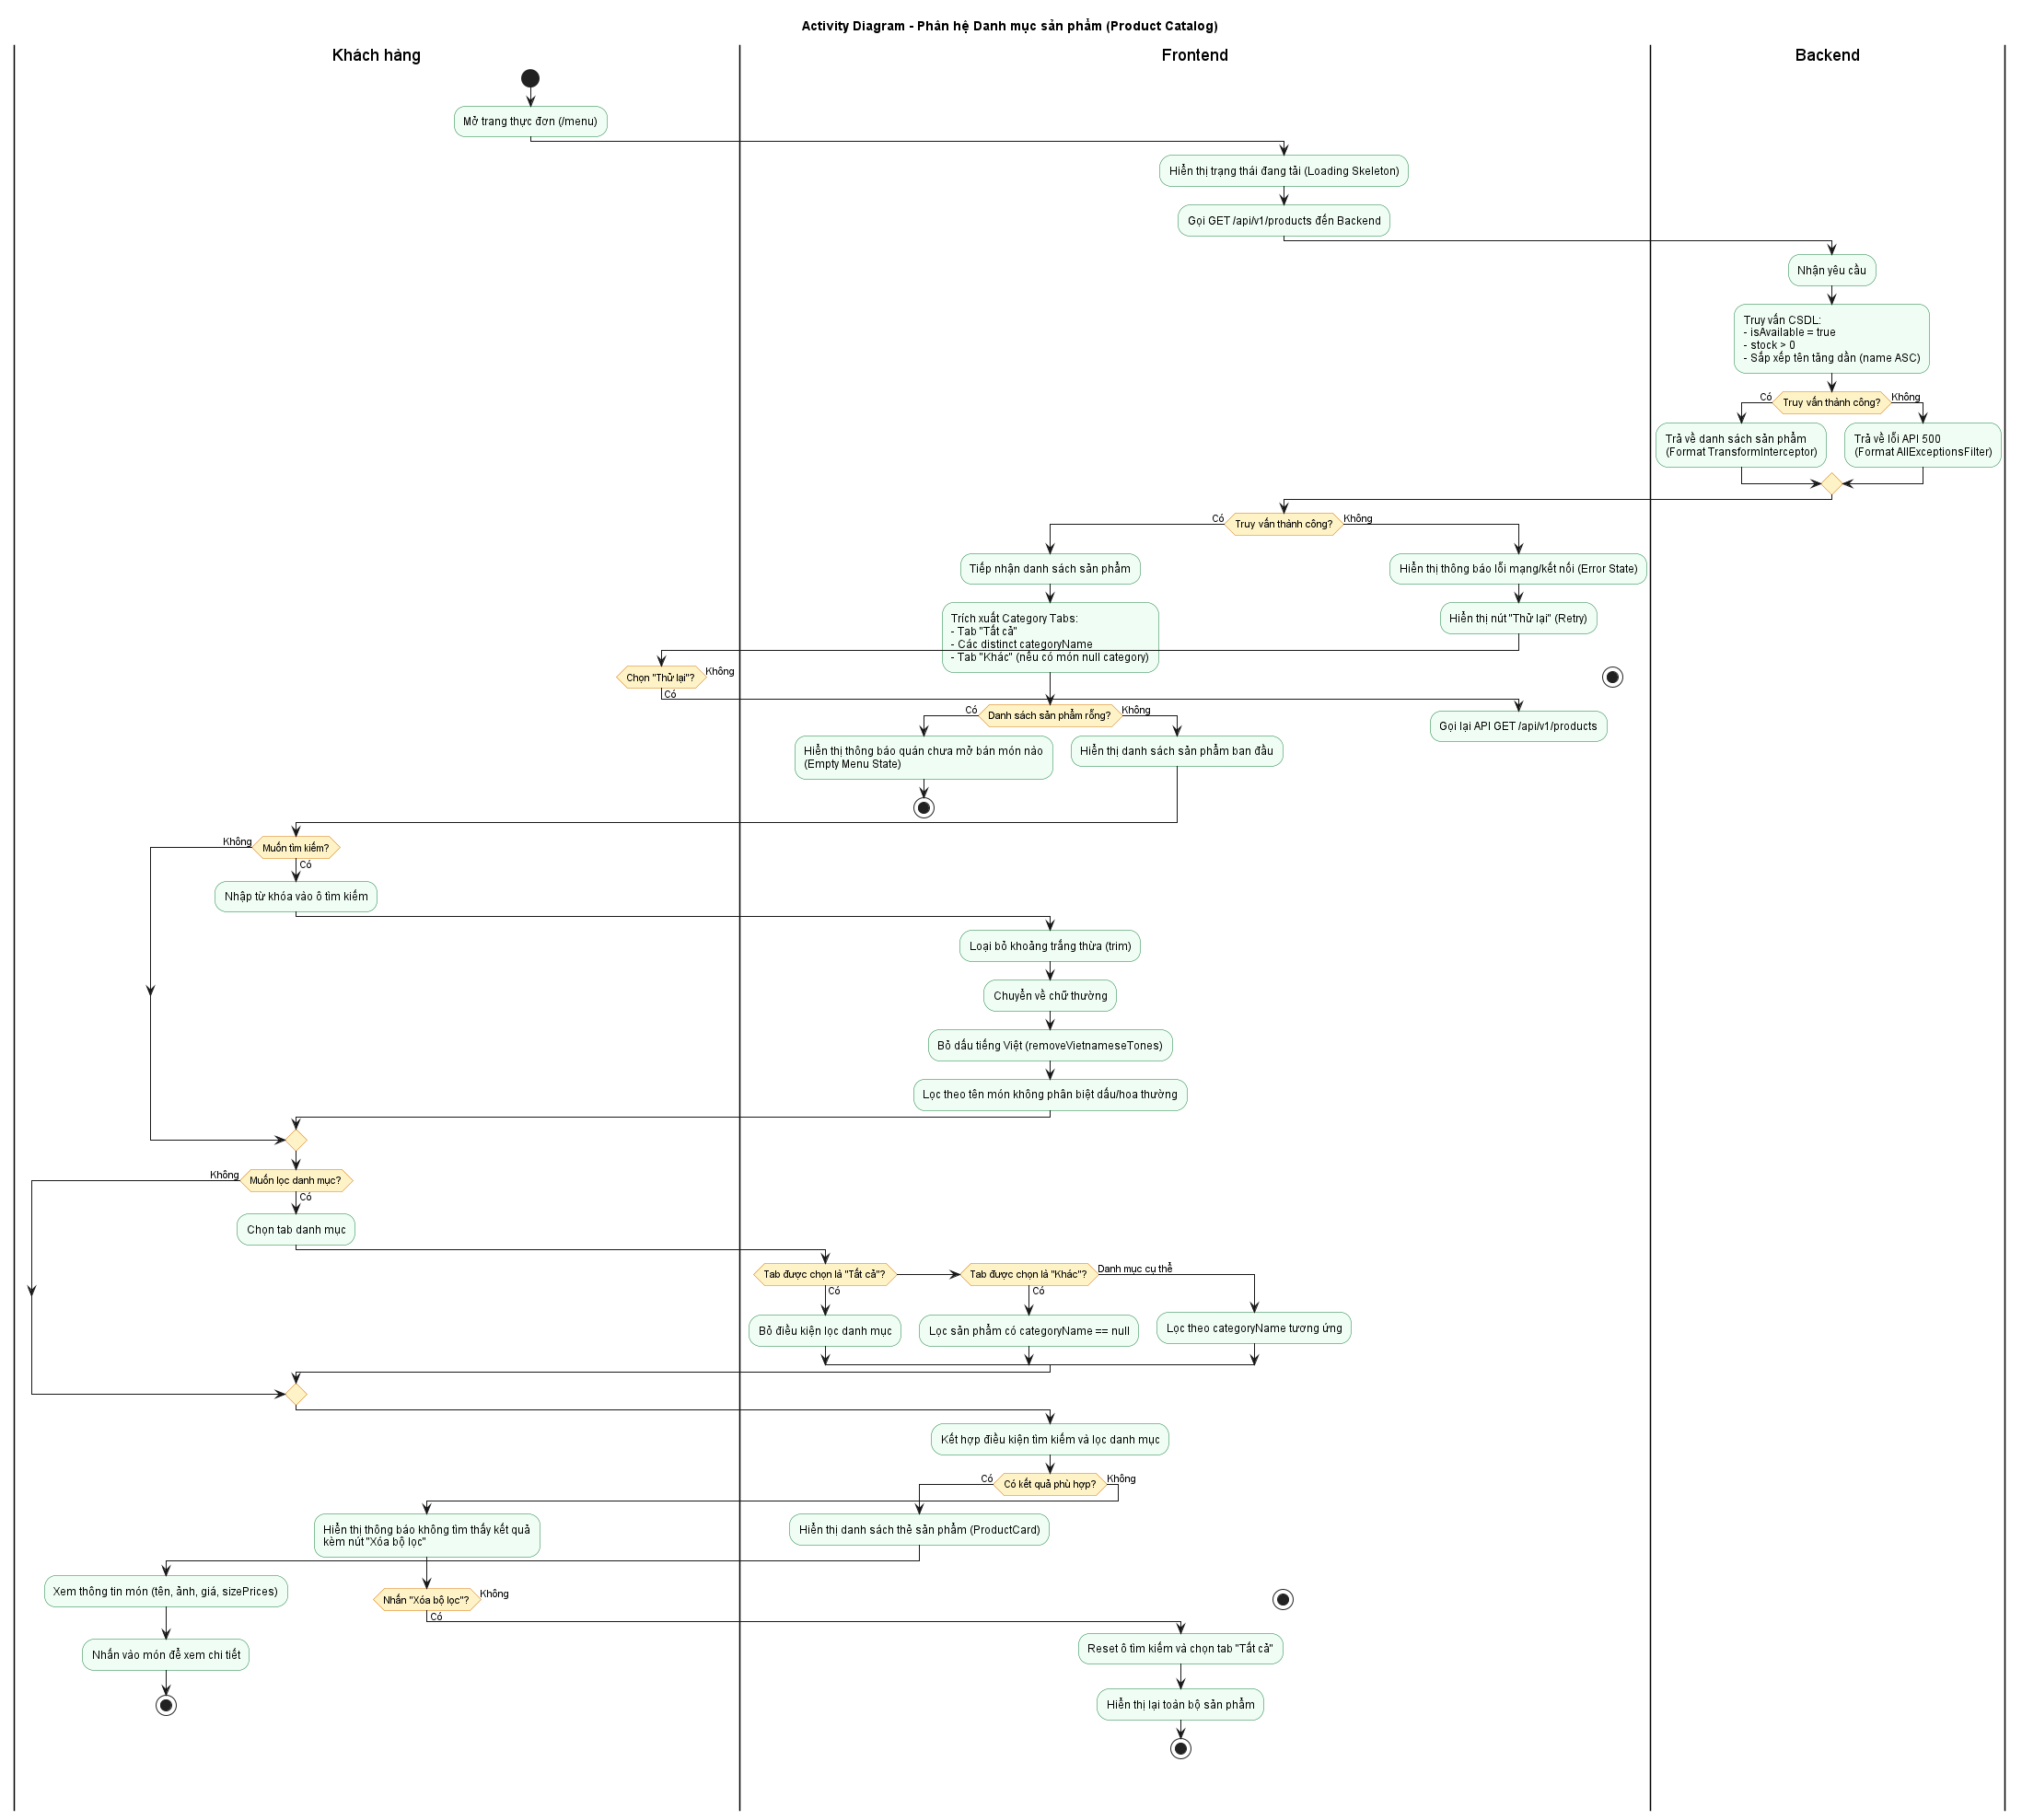
\includegraphics[width=0.88\textwidth,height=0.48\textheight,keepaspectratio]{../figures/diagrams/activity-product-catalog.png}
\caption{Activity Diagram: Quy trình duyệt thực đơn, lọc danh mục và tìm kiếm món}
\label{fig:ad-menu}
\end{figure}

% ---------------------------------------------------------------------
%  PHỤ LỤC B: QUẢN LÝ GIỎ HÀNG
% ---------------------------------------------------------------------
\clearpage
\section{Phân hệ Quản lý giỏ hàng (Cart Module)}
\label{app:cart}
Nguồn thiết kế: \file{cart (3).drawio}. Phân hệ giỏ hàng được quản lý phía Client thông qua Zustand Store kết hợp middleware persist (\code{localStorage}), hỗ trợ đầy đủ các thao tác thêm, chỉnh sửa cấu hình (size, topping), tăng giảm số lượng, tính tổng tạm tính và bảo toàn giỏ khi thanh toán thất bại.

\begin{figure}[H]
\centering
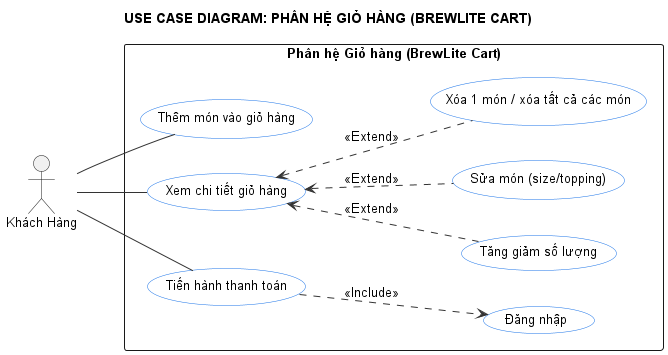
\includegraphics[width=0.85\textwidth,height=0.42\textheight,keepaspectratio]{../figures/diagrams/uc-cart.png}
\caption{Use Case Diagram: Phân hệ Quản lý giỏ hàng}
\label{fig:uc-cart}
\end{figure}

\begin{figure}[H]
\centering
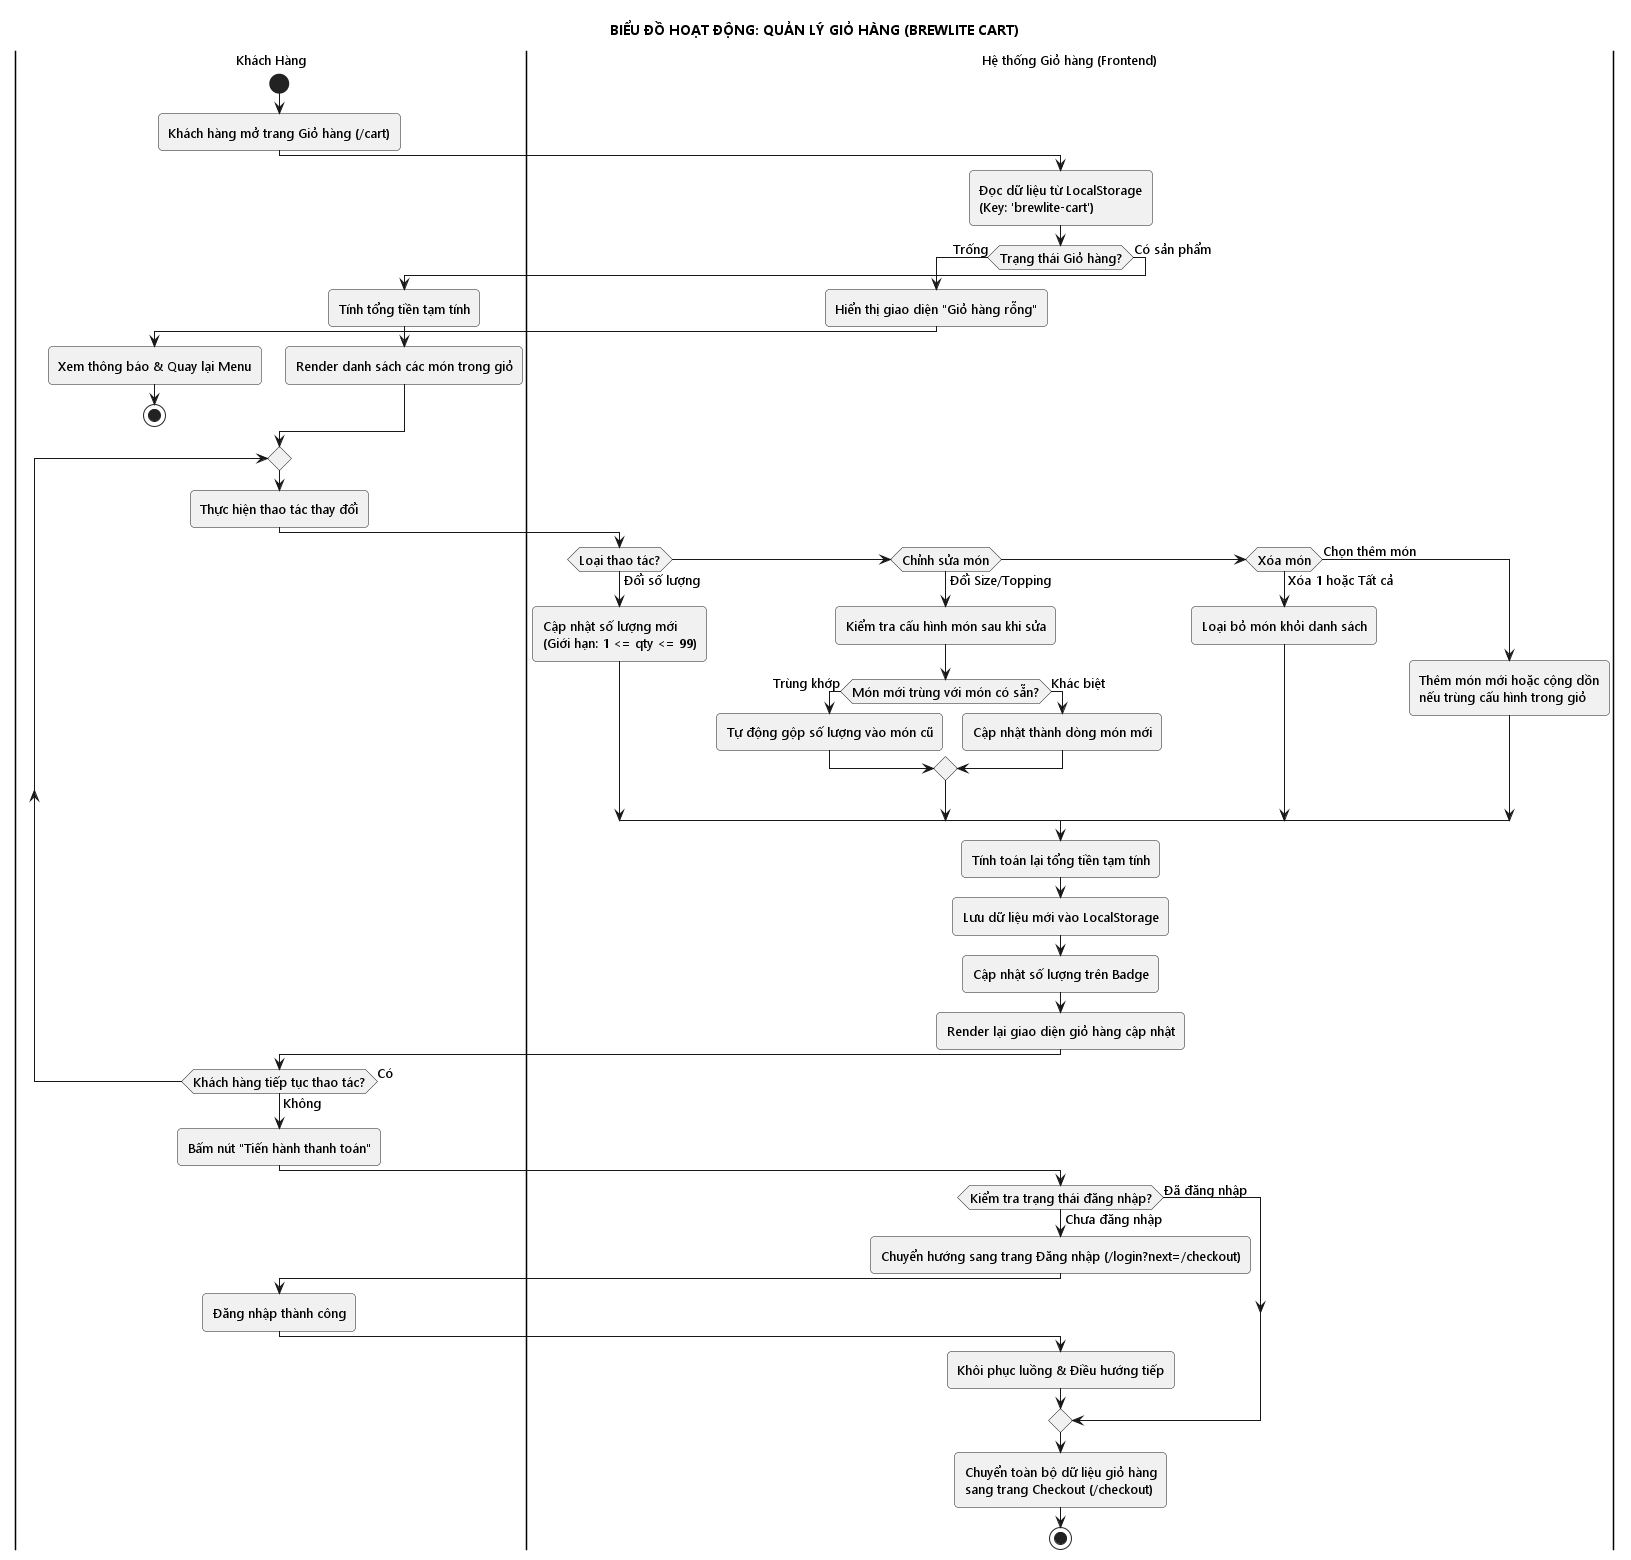
\includegraphics[width=0.88\textwidth,height=0.45\textheight,keepaspectratio]{../figures/diagrams/ad-cart.png}
\caption{Activity Diagram: Quy trình quản lý giỏ hàng}
\label{fig:ad-cart}
\end{figure}

\begin{figure}[H]
\centering
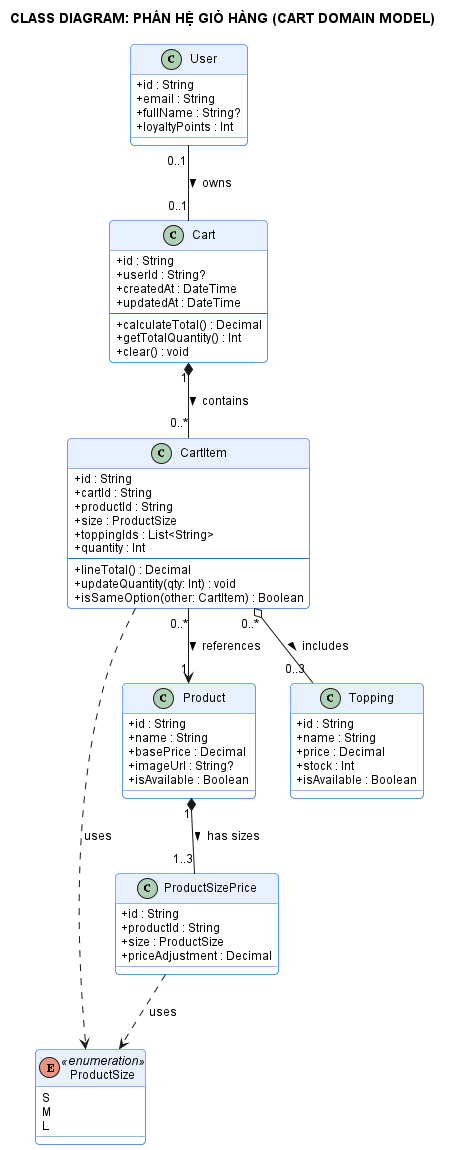
\includegraphics[width=0.85\textwidth,height=0.48\textheight,keepaspectratio]{../figures/diagrams/cd-cart.png}
\caption{Class Diagram: Mô hình dữ liệu Giỏ hàng (Cart Domain Model)}
\label{fig:cd-cart}
\end{figure}

\begin{figure}[H]
\centering
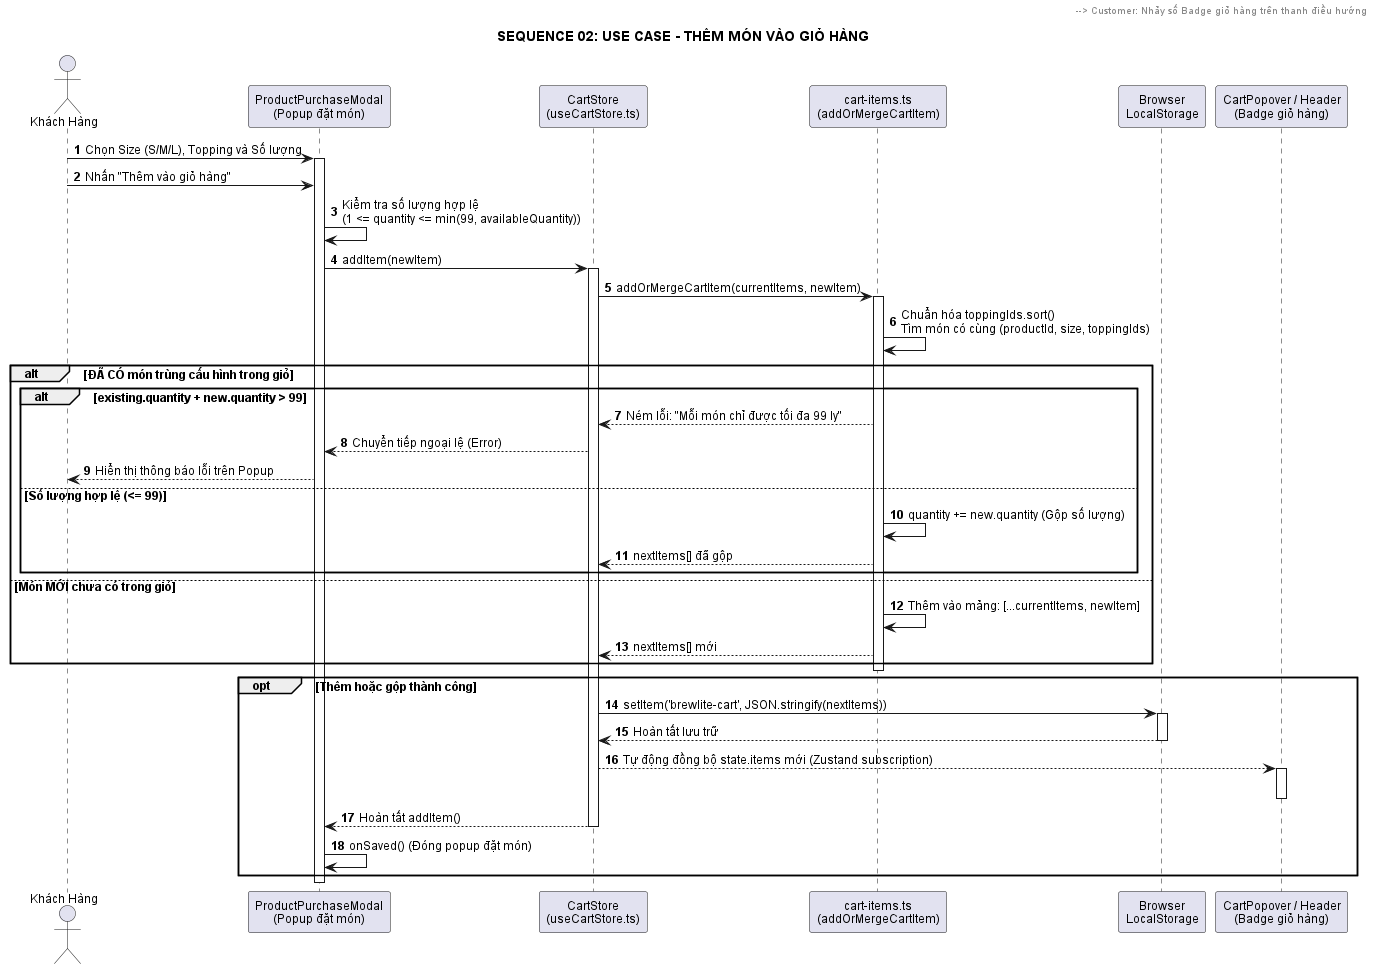
\includegraphics[width=0.88\textwidth,height=0.40\textheight,keepaspectratio]{../figures/diagrams/sd-cart-add.png}
\caption{Sequence Diagram: Thêm món vào giỏ hàng và gộp dòng trùng cấu hình}
\label{fig:sd-cart-add}
\end{figure}

\begin{figure}[H]
\centering
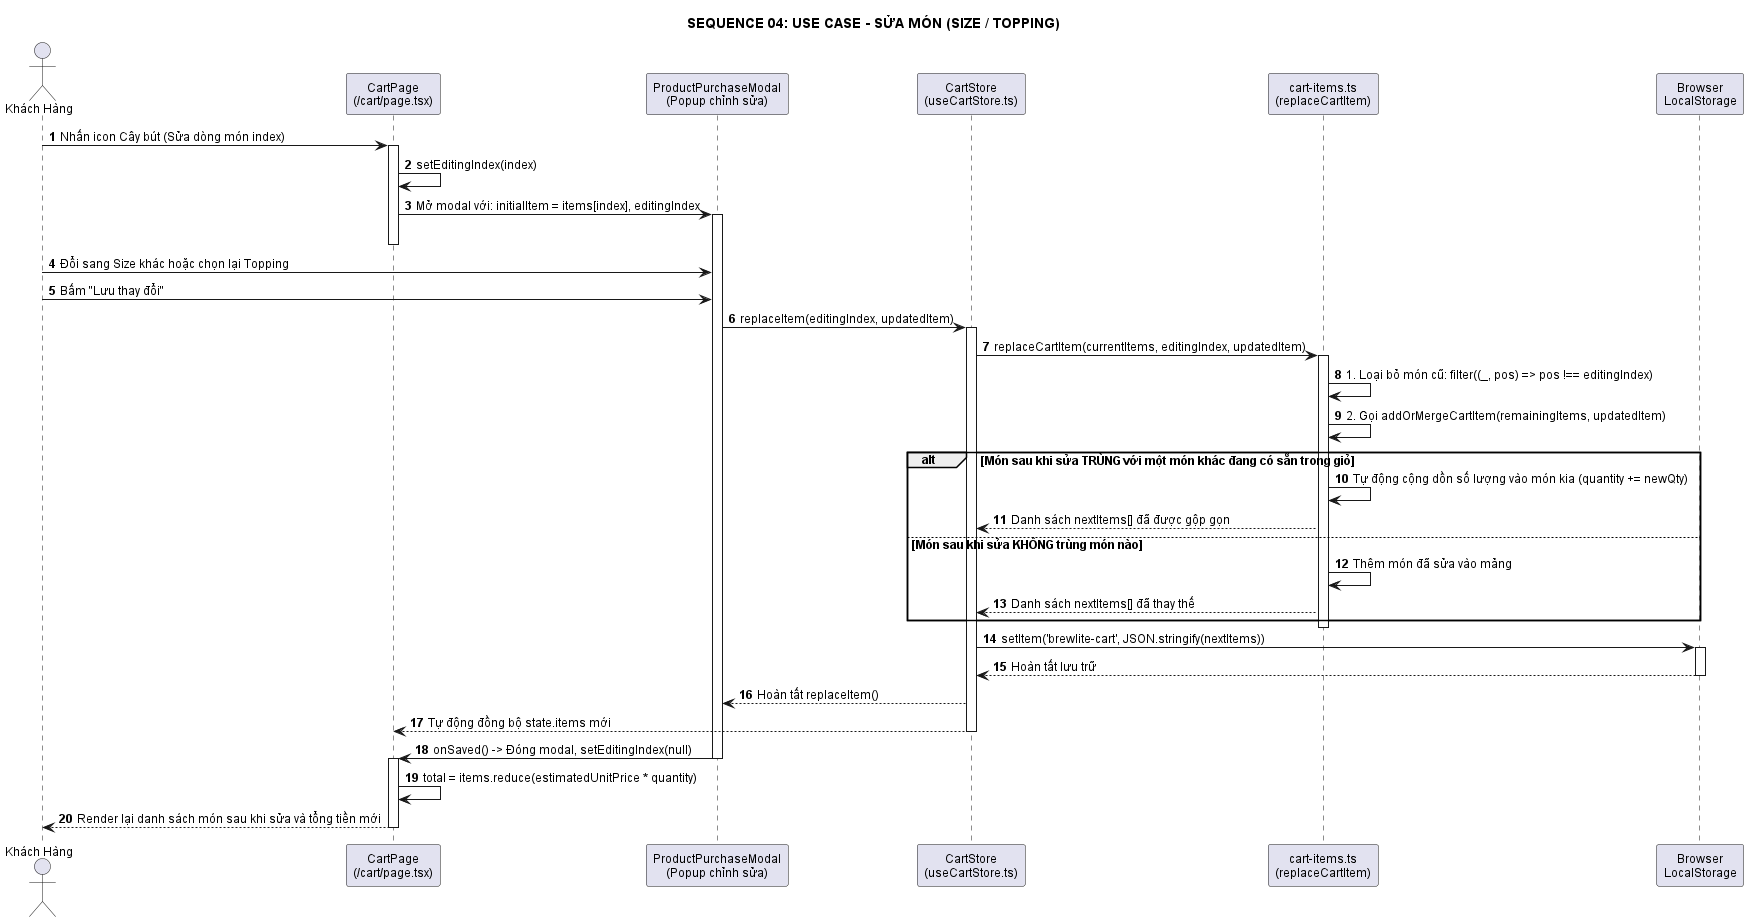
\includegraphics[width=0.88\textwidth,height=0.40\textheight,keepaspectratio]{../figures/diagrams/sd-cart-edit.png}
\caption{Sequence Diagram: Chỉnh sửa kích cỡ và topping của món trong giỏ}
\label{fig:sd-cart-edit}
\end{figure}

\begin{figure}[H]
\centering
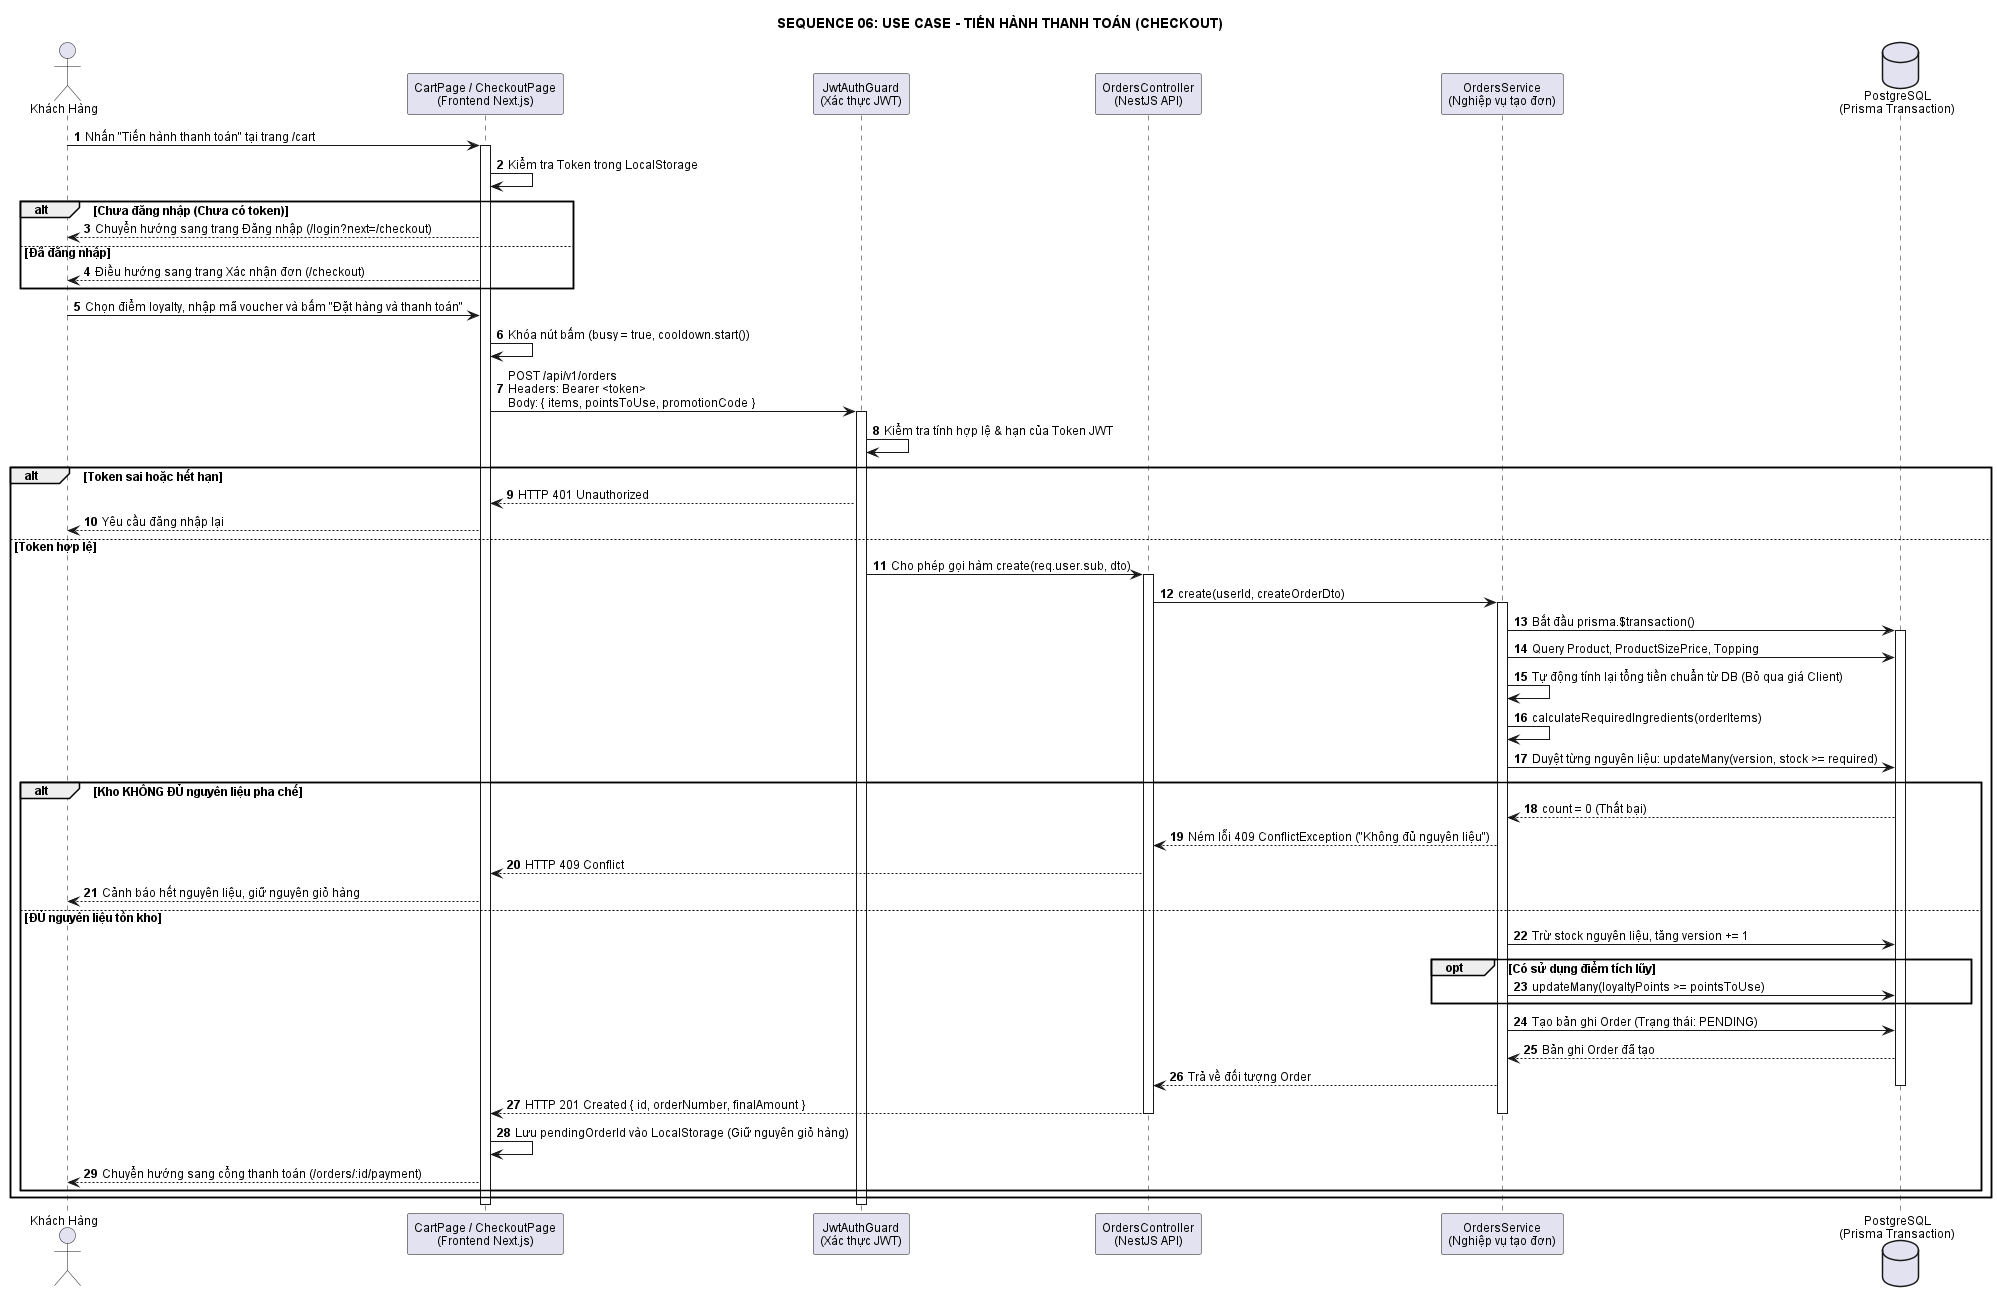
\includegraphics[width=0.88\textwidth,height=0.42\textheight,keepaspectratio]{../figures/diagrams/sd-cart-checkout.png}
\caption{Sequence Diagram: Tiến hành thanh toán từ giỏ hàng}
\label{fig:sd-cart-checkout}
\end{figure}

% ---------------------------------------------------------------------
%  PHỤ LỤC C: CHI TIẾT MÓN VÀ TÍNH GIÁ (PRODUCT DETAIL)
% ---------------------------------------------------------------------
\clearpage
\section{Phân hệ Chi tiết món và tính giá (Product Detail \& Pricing Module)}
\label{app:product-detail}

Phân hệ Chi tiết món và tính giá (Dải yêu cầu: FR-07..09) cho phép khách hàng xem đầy đủ thông tin chi tiết của một món đồ uống, tùy biến kích cỡ (Size S/M/L), chọn tối đa 3 loại topping, điều chỉnh số lượng và xem giá tạm tính cập nhật thời gian thực trước khi thêm vào giỏ hàng.

\subsection{Sơ đồ Use Case: Chi tiết và tùy biến món}
Sơ đồ mô tả các chức năng người dùng tương tác trên trang chi tiết sản phẩm (\file{/products/:id}), thể hiện các mối quan hệ $\ll include \gg$ kiểm tra tính toàn vẹn dữ liệu, khả năng mở bán và tính giá tạm tính.

\begin{figure}[H]
\centering
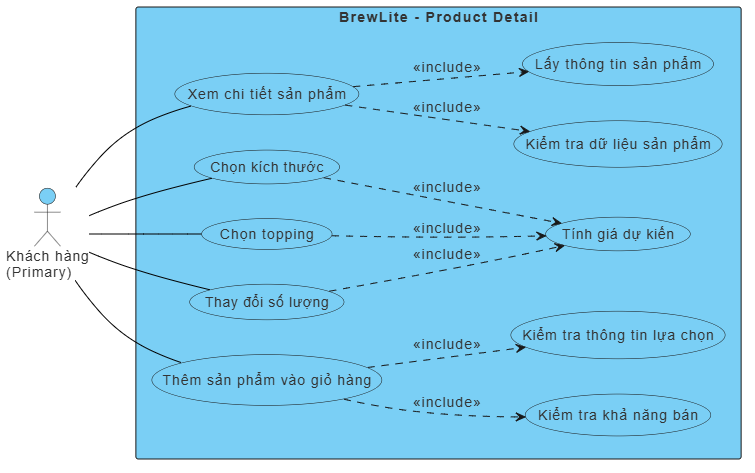
\includegraphics[width=0.88\textwidth]{../figures/diagrams/uc-product-detail-custom.png}
\caption{Use Case Diagram: Phân hệ Chi tiết món (BrewLite -- Product Detail)}
\label{fig:uc-product-detail-custom}
\end{figure}

\subsection{Sơ đồ tuần tự: Tải chi tiết, tùy biến và thêm vào giỏ}
Sơ đồ tuần tự gồm 3 giai đoạn phân ranh giới trách nhiệm rõ ràng:
\begin{enumerate}[label=\arabic*.]
  \item \textbf{Load Product Detail:} Client gọi API \code{GET /products/:id}. Frontend kiểm tra tính hợp lệ qua \code{isValidProduct(data)}, chọn size mặc định đầu tiên và nạp danh sách topping khả dụng. Trường hợp lỗi 404 hoặc lỗi mạng hiển thị giao diện báo lỗi chuyên biệt kèm nút thử lại.
  \item \textbf{Select Product Options:} Khi khách chọn kích cỡ, số lượng hoặc topping (kiểm soát chặt chẽ không quá 3 topping), giao diện tự động tính \code{estimatedPrice} và hiển thị giá tạm tính tức thì.
  \item \textbf{Add Product To Cart:} Kiểm tra tính khả dụng của món, tạo đối tượng \code{CartItemDraft}, đọc giỏ hàng từ \code{localStorage}, gộp dòng nếu trùng cấu hình (\code{addToCartMerge}), lưu lại bộ nhớ và phát sự kiện \code{cart-changed}.
\end{enumerate}

\begin{figure}[H]
\centering
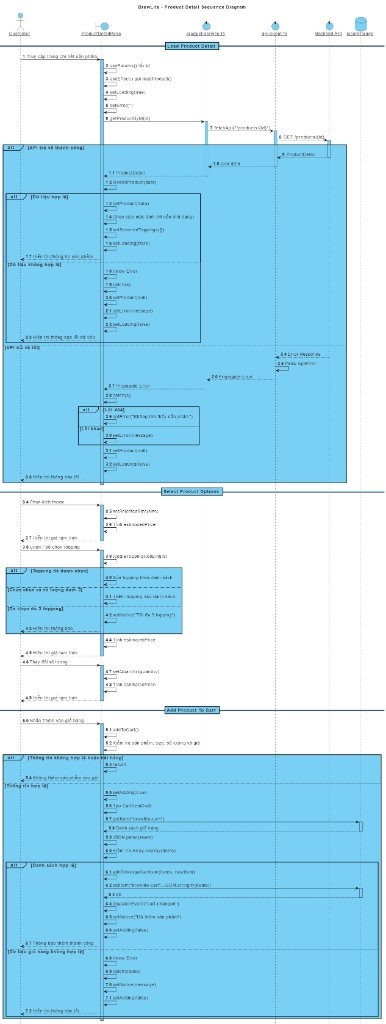
\includegraphics[height=0.84\textheight,keepaspectratio]{../figures/diagrams/sd-product-detail-custom.png}
\caption{Sequence Diagram: Tải chi tiết món, tùy biến và thêm vào giỏ hàng}
\label{fig:sd-product-detail-custom}
\end{figure}

\subsection{Sơ đồ hoạt động: Quy trình chi tiết món End-to-End}
Sơ đồ hoạt động thể hiện luồng điều khiển nghiệp vụ giữa 3 làn: \textbf{Khách hàng}, \textbf{Frontend (Next.js)} và \textbf{Backend (NestJS API)}.

\begin{figure}[H]
\centering
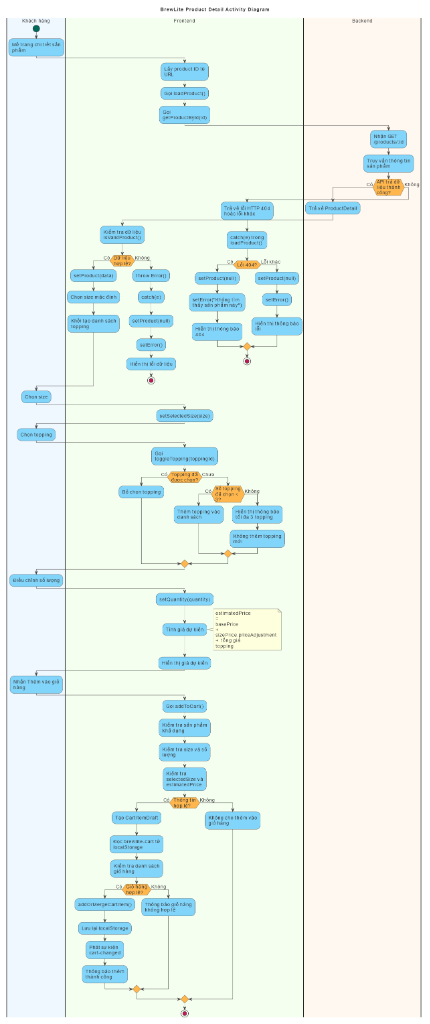
\includegraphics[height=0.84\textheight,keepaspectratio]{../figures/diagrams/ad-product-detail-custom.png}
\caption{Activity Diagram: Quy trình hiển thị, tùy biến và thêm giỏ hàng}
\label{fig:ad-product-detail-custom}
\end{figure}

\subsection{Nguyên tắc kiến trúc và công thức tính giá chuẩn}
\paragraph{Nguyên tắc kiến trúc bắt buộc:}
\begin{enumerate}[label=\arabic*.]
  \item \textbf{Backend là nguồn sự thật duy nhất về giá (Single Source of Truth):} Mọi công thức tính đơn giá, phụ thu và thành tiền bắt buộc do \code{PricingService.calculate()} ở Backend đọc trực tiếp từ PostgreSQL và tính toán độc lập. Client không được phép gửi giá tính sẵn để quyết định số tiền phải trả.
  \item \textbf{Frontend chỉ hiển thị giá tạm tính (Estimated Price Only):} Giao diện chỉ hiển thị giá ước tính phục vụ trải nghiệm người dùng tức thời; giá thanh toán chính thức chỉ được chốt lại khi tạo đơn (\code{OrdersService.create()}).
  \item \textbf{Toàn vẹn số học VNĐ:} Tiền tệ sử dụng số nguyên chuẩn VNĐ (\code{Decimal(12, 0)} trong CSDL), không làm tròn sai số dấu phẩy động.
\end{enumerate}

\paragraph{Công thức tính giá chuẩn (Pricing Formula):}
$$\text{unitPrice} = \text{basePrice} + \text{priceAdjustment}(\text{size})$$
$$\text{toppingTotal} = \sum_{i=1}^{k} \text{toppingPrice}_i \quad (0 \le k \le 3)$$
$$\text{unitPriceWithToppings} = \text{unitPrice} + \text{toppingTotal}$$
$$\text{lineTotal} = \text{unitPriceWithToppings} \times \text{quantity} \quad (1 \le \text{quantity} \le 99)$$
$$\text{subtotal} = \sum \text{lineTotal}$$

\subsection{Đặc tả yêu cầu chức năng và tiêu chí chấp nhận (FR-07..09)}

\begin{table}[H]
\centering\footnotesize
\caption{Đặc tả các yêu cầu chức năng phân hệ Chi tiết món}
\label{tab:fr-detail-specs}
\begin{tabularx}{\textwidth}{@{}p{1.4cm} p{3.2cm} X@{}}
\toprule
\textbf{Mã FR} & \textbf{Yêu cầu nghiệp vụ} & \textbf{Tiêu chí chấp nhận chính (Acceptance Criteria)} \\
\midrule
FR-07 & Xem chi tiết sản phẩm (Product Detail View) &
  \textbf{AC-07.1:} Tải dữ liệu từ \code{GET /api/v1/products/:id}, hiển thị tên, ảnh (ảnh fallback khi null), giá gốc, size, topping khả dụng.\newline
  \textbf{AC-07.2:} ID không tồn tại trả \code{404 Not Found}, hiển thị màn hình lỗi và nút quay lại menu.\newline
  \textbf{AC-07.4:} Món ngừng bán (\code{isAvailable = false}) hiển thị huy hiệu ``Hết hàng'' và vô hiệu hóa nút thêm vào giỏ. \\
\midrule
FR-08 & Tùy biến kích cỡ và Topping (Customization) &
  \textbf{AC-08.1:} Radio group chọn duy nhất 1 size, mặc định chọn Size S.\newline
  \textbf{AC-08.2:} Chọn từ 0 đến tối đa 3 topping không trùng lặp. Đạt 3 topping tự động khóa checkbox còn lại; bỏ chọn mở khóa lại.\newline
  \textbf{AC-08.3:} Tăng/giảm số lượng trong biên nguyên $[1, 99]$; nút giảm vô hiệu ở 1, nút tăng vô hiệu ở 99. \\
\midrule
FR-09 & Tính giá tạm tính \& Xác thực Backend &
  \textbf{AC-09.1:} Cập nhật giá tức thì trên UI khi đổi size (+5.000đ cho Size M, +10.000đ cho Size L).\newline
  \textbf{AC-09.2:} Cập nhật giá tức thì khi thêm/bớt topping (+5.000đ trân châu, +10.000đ kem cheese...).\newline
  \textbf{AC-09.4:} Backend tính lại độc lập theo công thức từ DB, không nhận giá do Client gửi lên. \\
\bottomrule
\end{tabularx}
\end{table}

\begin{table}[H]
\centering\footnotesize
\caption{Ánh xạ tiêu chí chấp nhận (AC) phân hệ Chi tiết món sang Test Case ID}
\label{tab:mapping-ac-detail}
\begin{tabularx}{\textwidth}{@{}p{1.8cm} X p{2.5cm} p{2.8cm}@{}}
\toprule
\textbf{Mã AC} & \textbf{Kịch bản kiểm chứng} & \textbf{Loại test} & \textbf{Test Case ID} \\
\midrule
AC-07.1 & Lấy \& hiển thị chi tiết sản phẩm hợp lệ & Component / Int & TC-DETAIL-01 \\
AC-07.2 & Sản phẩm không tồn tại trả về 404 & Component / Int & TC-DETAIL-02 \\
AC-07.3 & ID sai định dạng hoặc lỗi kết nối trả về 400 & Component / Int & TC-DETAIL-06 \\
AC-07.4 & Sản phẩm ngừng bán / hết hàng hiển thị cảnh báo & Component & TC-DETAIL-07 \\
AC-08.1 & Chọn kích cỡ duy nhất \& mặc định Size S trên UI & Component & TC-DETAIL-03 \\
AC-08.2 & Chọn/bỏ chọn Topping \& chặn vượt quá 3 loại & Component & TC-DETAIL-04 \\
AC-08.3 & Điều chỉnh số lượng trong biên nguyên 1..99 & Component & TC-DETAIL-08 \\
AC-08.4 & Chặn thêm giỏ khi thiếu thuộc tính size bắt buộc & Component & TC-DETAIL-09 \\
AC-09.1 & Cập nhật giá realtime khi chọn/đổi Size trên UI & Component & TC-DETAIL-10 \\
AC-09.2 & Cập nhật giá realtime khi thêm/bớt Topping trên UI & Component & TC-DETAIL-11 \\
AC-09.3 & Cập nhật thành tiền khi đổi số lượng \& lưu vào Giỏ & Component & TC-DETAIL-12 \\
AC-09.4 & Backend tính lại giá độc lập theo DB, không làm tròn & Unit & TC-DETAIL-05 \\
AC-09.5 & Backend bảo vệ tính toàn vẹn giá, chống giả mạo & Unit & TC-DETAIL-05 \\
AC-09.6 & Backend từ chối dữ liệu đầu vào \& trạng thái DB sai & Unit & TC-DETAIL-13 \\
\bottomrule
\end{tabularx}
\end{table}

\subsection{Mô hình quản lý công thức sản phẩm phía Quản trị (Admin BOM)}
Bên cạnh giao diện người dùng, quản trị viên thiết lập công thức sản phẩm (\file{ProductRecipe}) liên kết từng kích cỡ với nguyên liệu kho (\file{Ingredient}) để làm cơ sở trừ kho khi đặt hàng:

\begin{figure}[H]
\centering
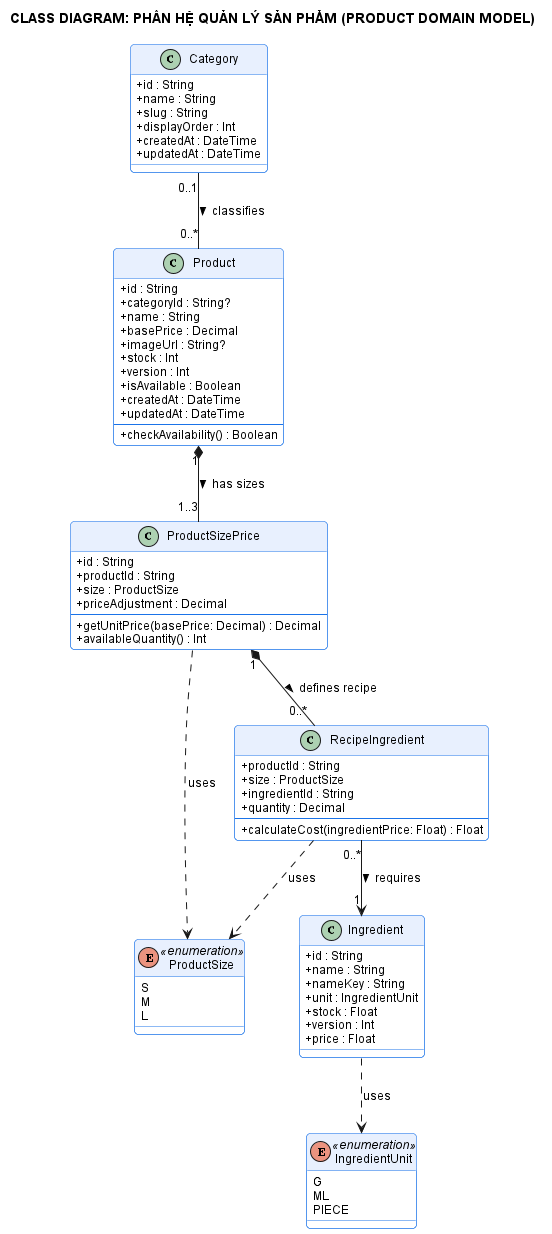
\includegraphics[width=0.85\textwidth,height=0.45\textheight,keepaspectratio]{../figures/diagrams/cd-product.png}
\caption{Class Diagram: Mô hình quan hệ Sản phẩm, Kích cỡ và Công thức (Admin)}
\label{fig:cd-product}
\end{figure}

% ---------------------------------------------------------------------
%  PHỤ LỤC D: QUẢN LÝ NGUYÊN LIỆU & NHẬP KHO
% ---------------------------------------------------------------------
\clearpage
\section{Phân hệ Quản lý nguyên liệu và nhập kho (Ingredients Management)}
\label{app:ingredients}
Nguồn thiết kế: \file{quản lý nguyên liệu ingredients cho brewlite.drawio}. Cung cấp khả năng theo dõi tồn kho nguyên liệu thời gian thực theo đơn vị đo (g, ml, piece), phát hiện cảnh báo dưới ngưỡng định mức an toàn, và quy trình lập phiếu nhập kho theo lô.

\begin{figure}[H]
\centering
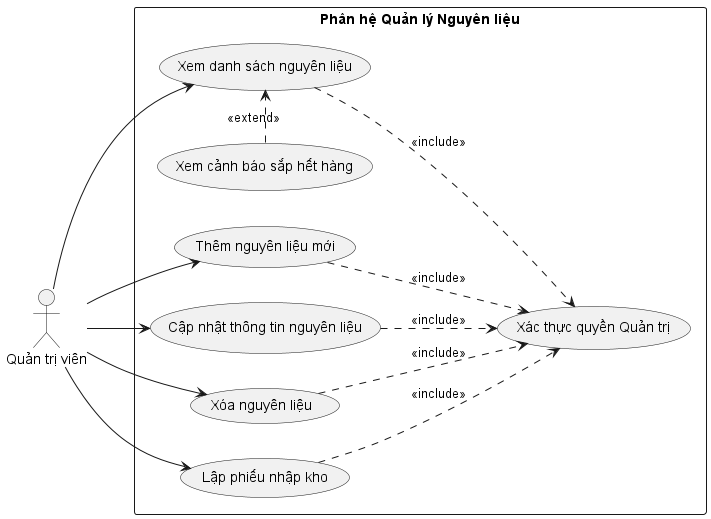
\includegraphics[width=0.75\textwidth,height=0.40\textheight,keepaspectratio]{../figures/diagrams/uc-ingredient-mgmt.png}
\caption{Use Case Diagram: Quản lý kho nguyên liệu và nhập kho}
\label{fig:uc-ingredient-mgmt}
\end{figure}

\begin{figure}[H]
\centering
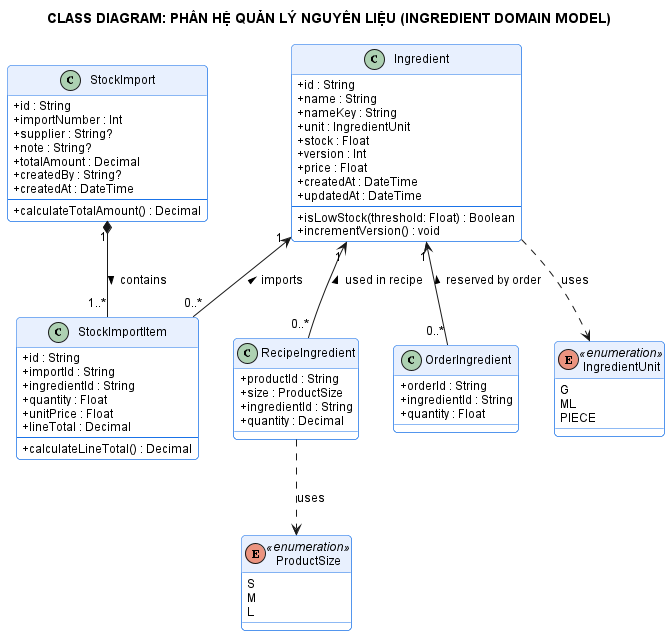
\includegraphics[width=0.85\textwidth,height=0.48\textheight,keepaspectratio]{../figures/diagrams/cd-ingredient.png}
\caption{Class Diagram: Mô hình dữ liệu Nguyên liệu và Phiếu nhập kho}
\label{fig:cd-ingredient}
\end{figure}

\begin{figure}[H]
\centering
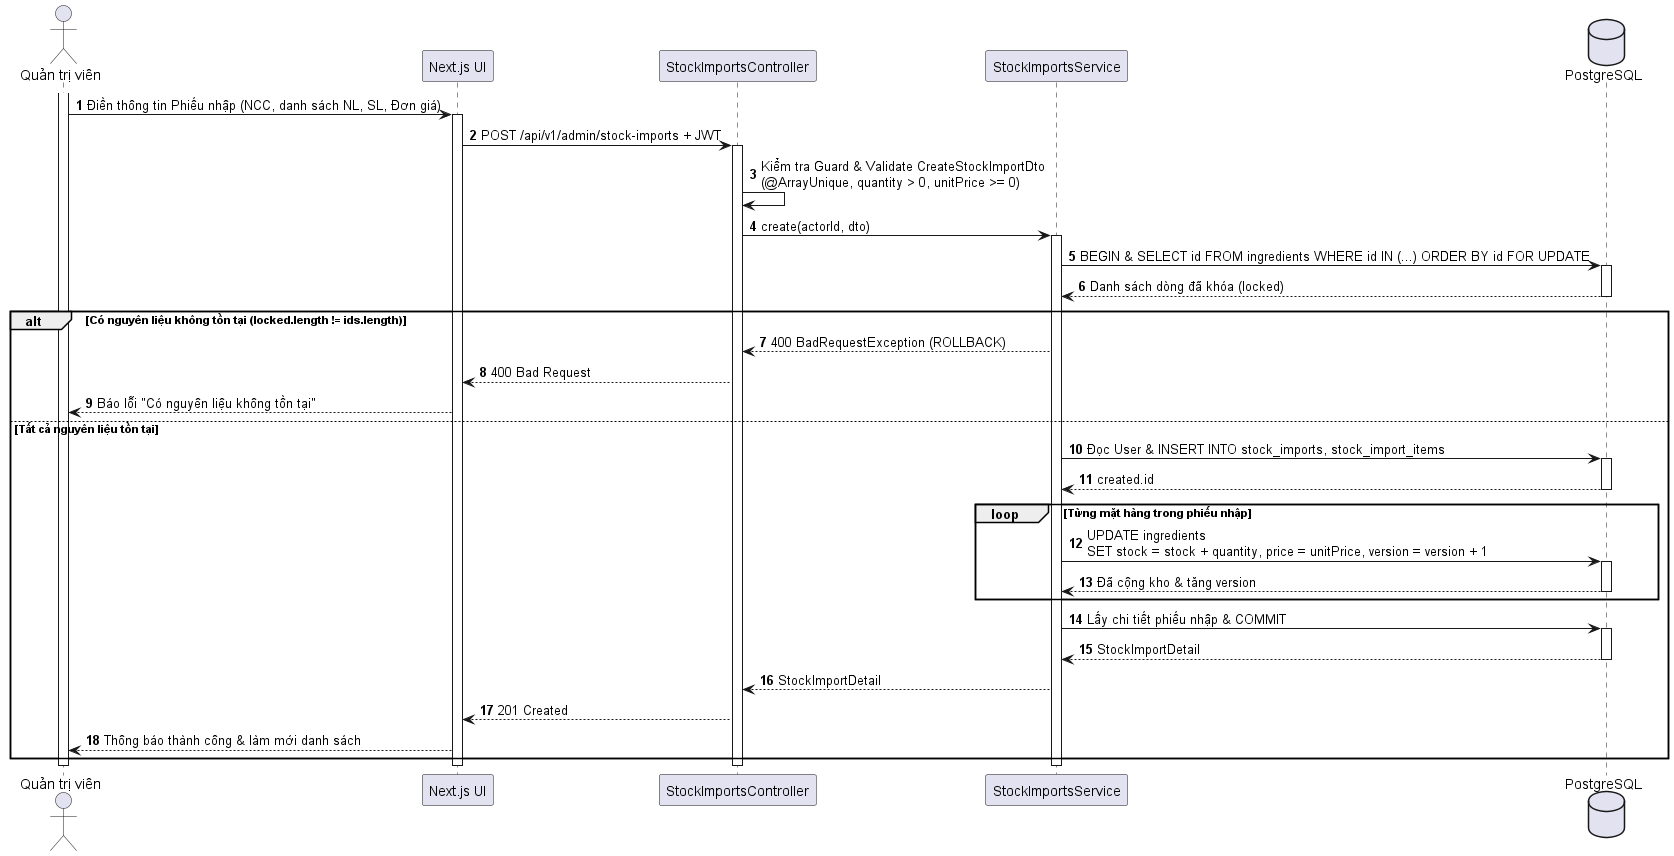
\includegraphics[width=0.88\textwidth,height=0.42\textheight,keepaspectratio]{../figures/diagrams/sd-ingredient-import.png}
\caption{Sequence Diagram: Quy trình lập phiếu nhập kho nguyên liệu}
\label{fig:sd-ingredient-import}
\end{figure}

\begin{figure}[H]
\centering
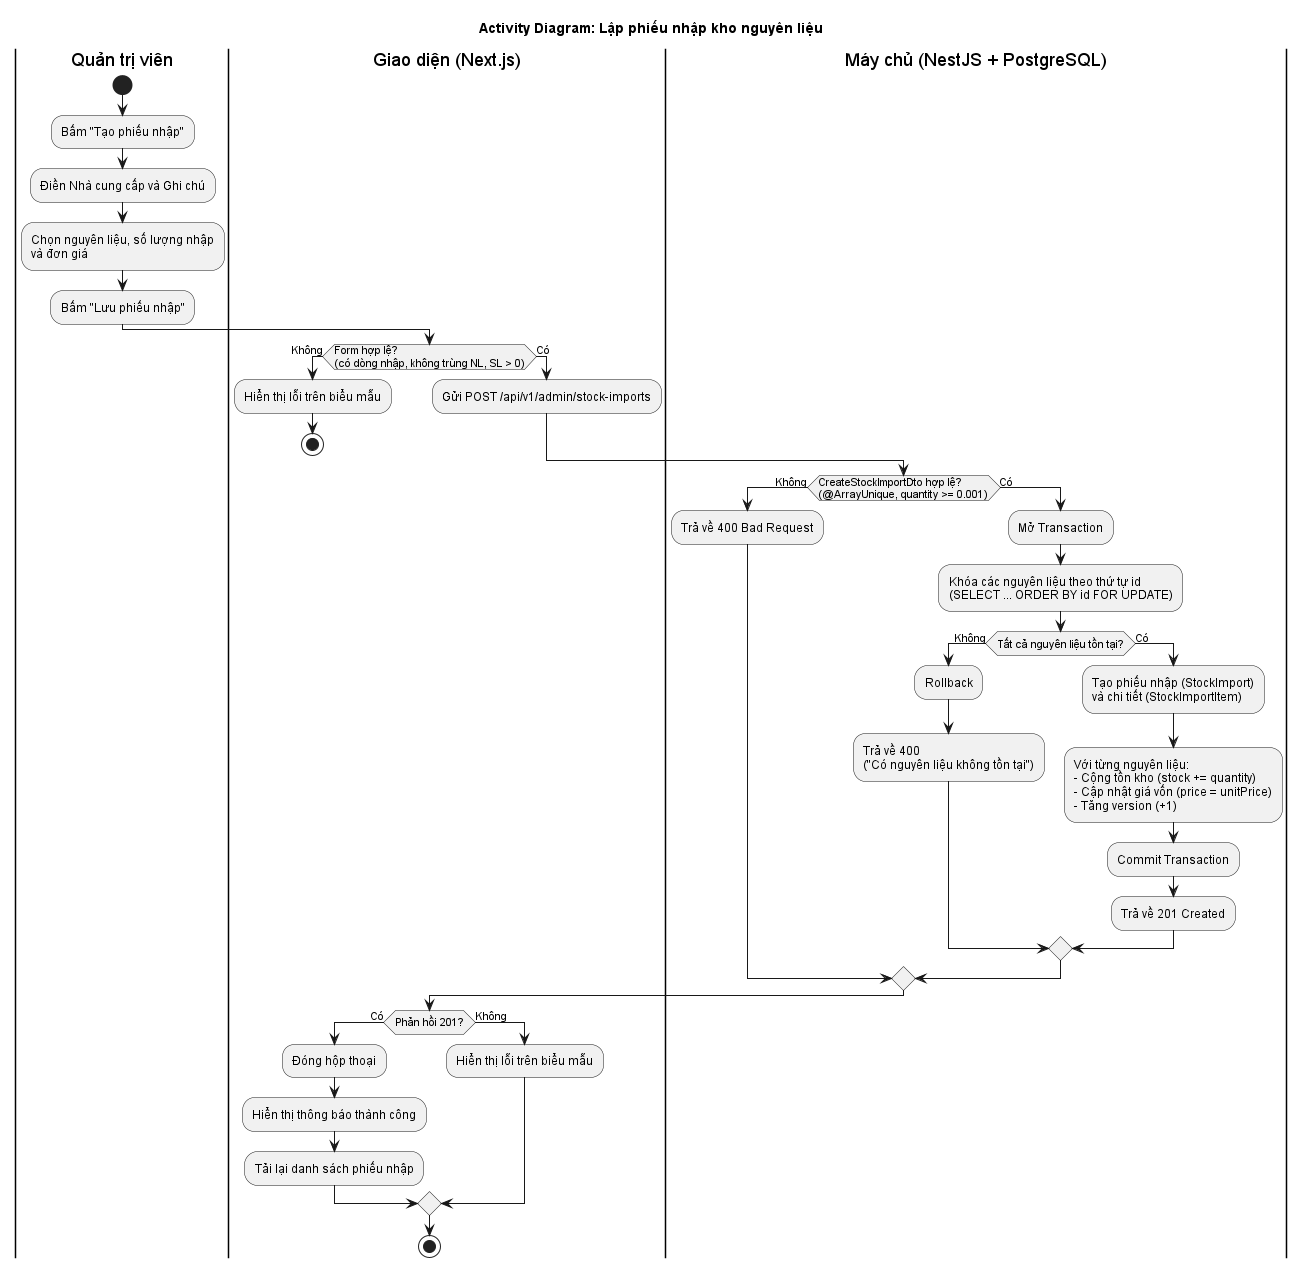
\includegraphics[width=0.88\textwidth,height=0.42\textheight,keepaspectratio]{../figures/diagrams/ad-ingredient-import.png}
\caption{Activity Diagram: Quy trình nhập kho nguyên liệu}
\label{fig:ad-ingredient-import}
\end{figure}

% ---------------------------------------------------------------------
%  PHỤ LỤC E: LỊCH SỬ ĐƠN HÀNG
% ---------------------------------------------------------------------
\clearpage
\section{Phân hệ Lịch sử đơn hàng (Order History Module)}
\label{app:history}
Nguồn thiết kế: \file{Order\&OrderHistory.drawio}. Cho phép khách hàng theo dõi danh sách các đơn đã đặt, xem chi tiết từng đơn hàng kèm mã biên nhận, trạng thái pha chế thời gian thực (tự động polling mỗi 10 giây khi đơn ở PAID, PREPARING, READY), và kiểm tra số điểm tích lũy.

\begin{figure}[H]
\centering
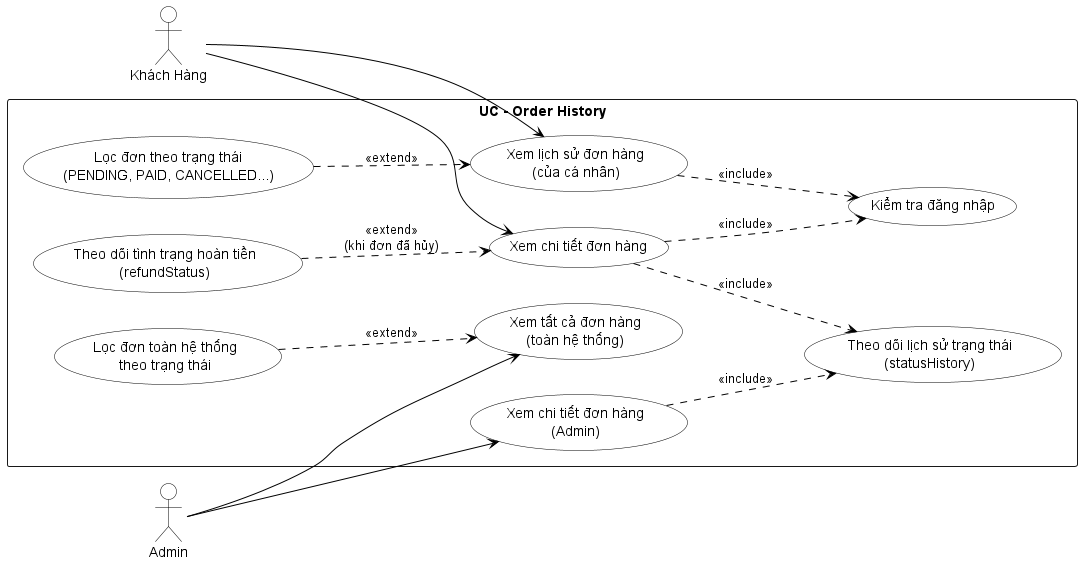
\includegraphics[width=0.82\textwidth,height=0.40\textheight,keepaspectratio]{../figures/diagrams/uc-order-history.png}
\caption{Use Case Diagram: Phân hệ Lịch sử đơn hàng}
\label{fig:uc-order-history}
\end{figure}

\begin{figure}[H]
\centering
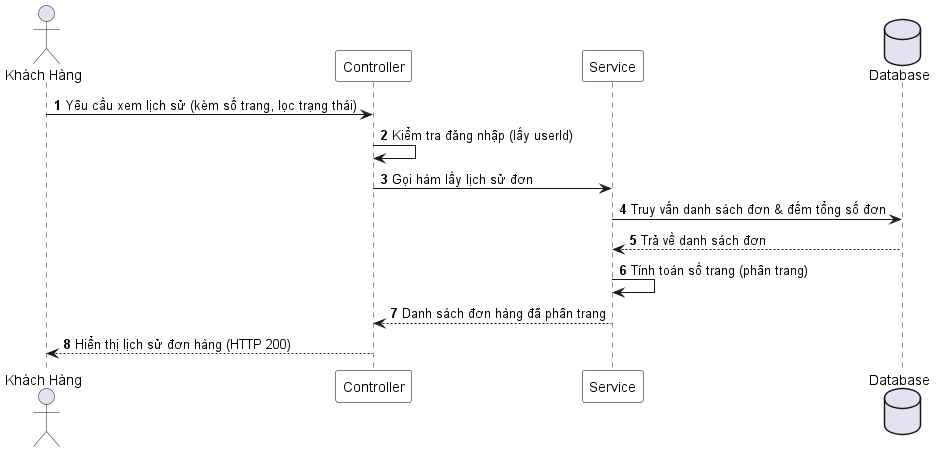
\includegraphics[width=0.88\textwidth,height=0.42\textheight,keepaspectratio]{../figures/diagrams/sd-order-history-list.png}
\caption{Sequence Diagram: Xem danh sách lịch sử đơn hàng cá nhân}
\label{fig:sd-order-history-list}
\end{figure}

\begin{figure}[H]
\centering
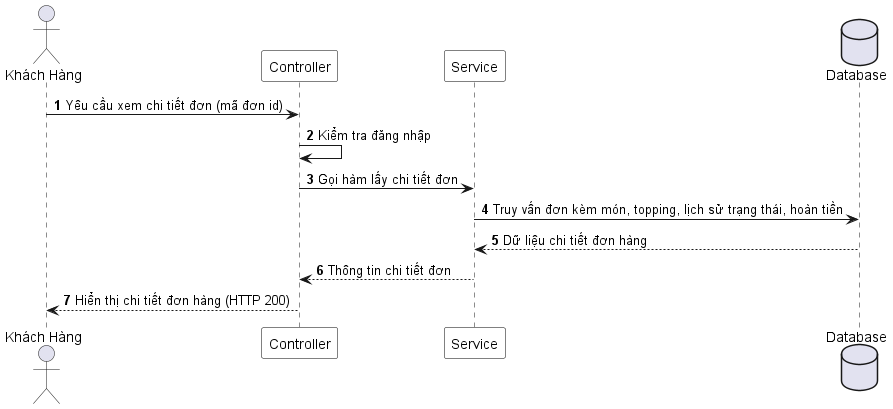
\includegraphics[width=0.88\textwidth,height=0.42\textheight,keepaspectratio]{../figures/diagrams/sd-order-history-detail.png}
\caption{Sequence Diagram: Xem chi tiết đơn hàng và polling trạng thái}
\label{fig:sd-order-history-detail}
\end{figure}

\begin{figure}[H]
\centering
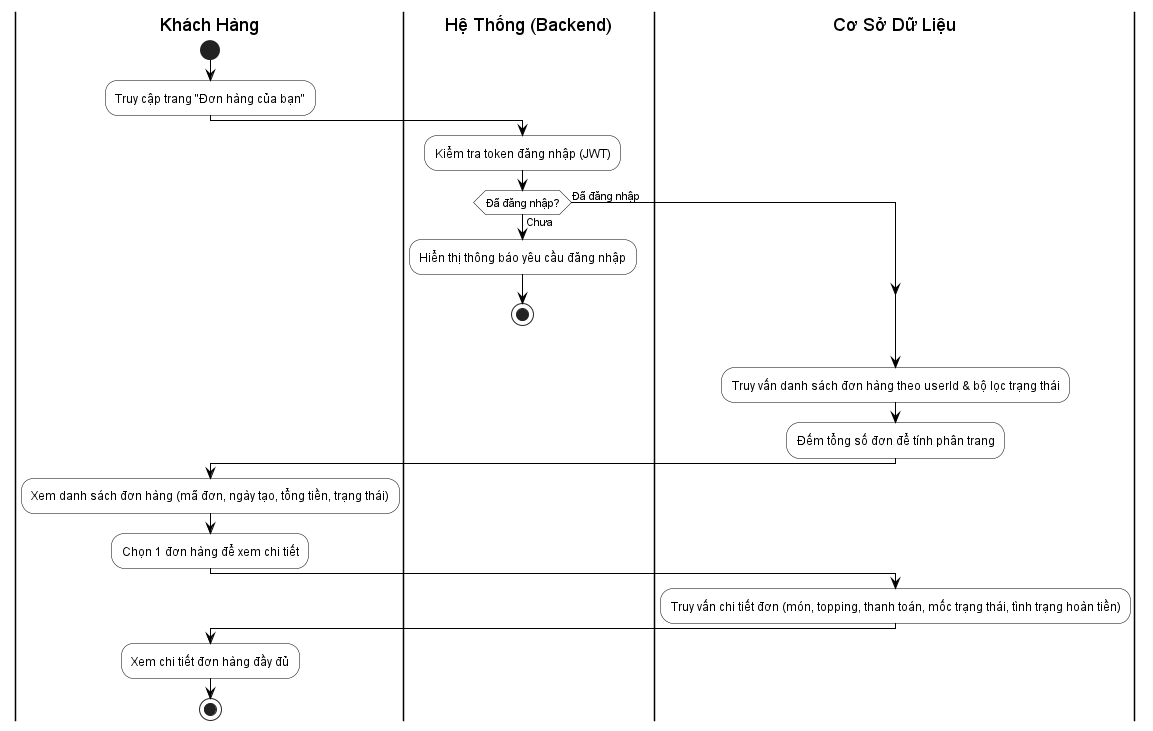
\includegraphics[width=0.88\textwidth,height=0.42\textheight,keepaspectratio]{../figures/diagrams/ad-order-history.png}
\caption{Activity Diagram: Quy trình truy vấn lịch sử và chi tiết đơn hàng}
\label{fig:ad-order-history}
\end{figure}

% =====================================================================
%  Phụ lục F: Phân hệ Cổng thanh toán ZaloPay Sandbox
%  Nguồn: backend/src/modules/payments/zalopay-sandbox.*
% =====================================================================
\section{Phân hệ Cổng thanh toán ZaloPay Sandbox (ZaloPay Sandbox Module)}
\label{app:zalopay-sandbox}

Tài liệu này mô tả hành vi đang có trong mã nguồn dự án đối với việc tích hợp cổng thanh toán trực tuyến qua môi trường thử nghiệm ZaloPay Sandbox, với ranh giới hệ thống là ứng dụng BrewLite.

\subsection{Tổng quan kiến trúc và các Actor bên ngoài}

\begin{figure}[H]
\centering
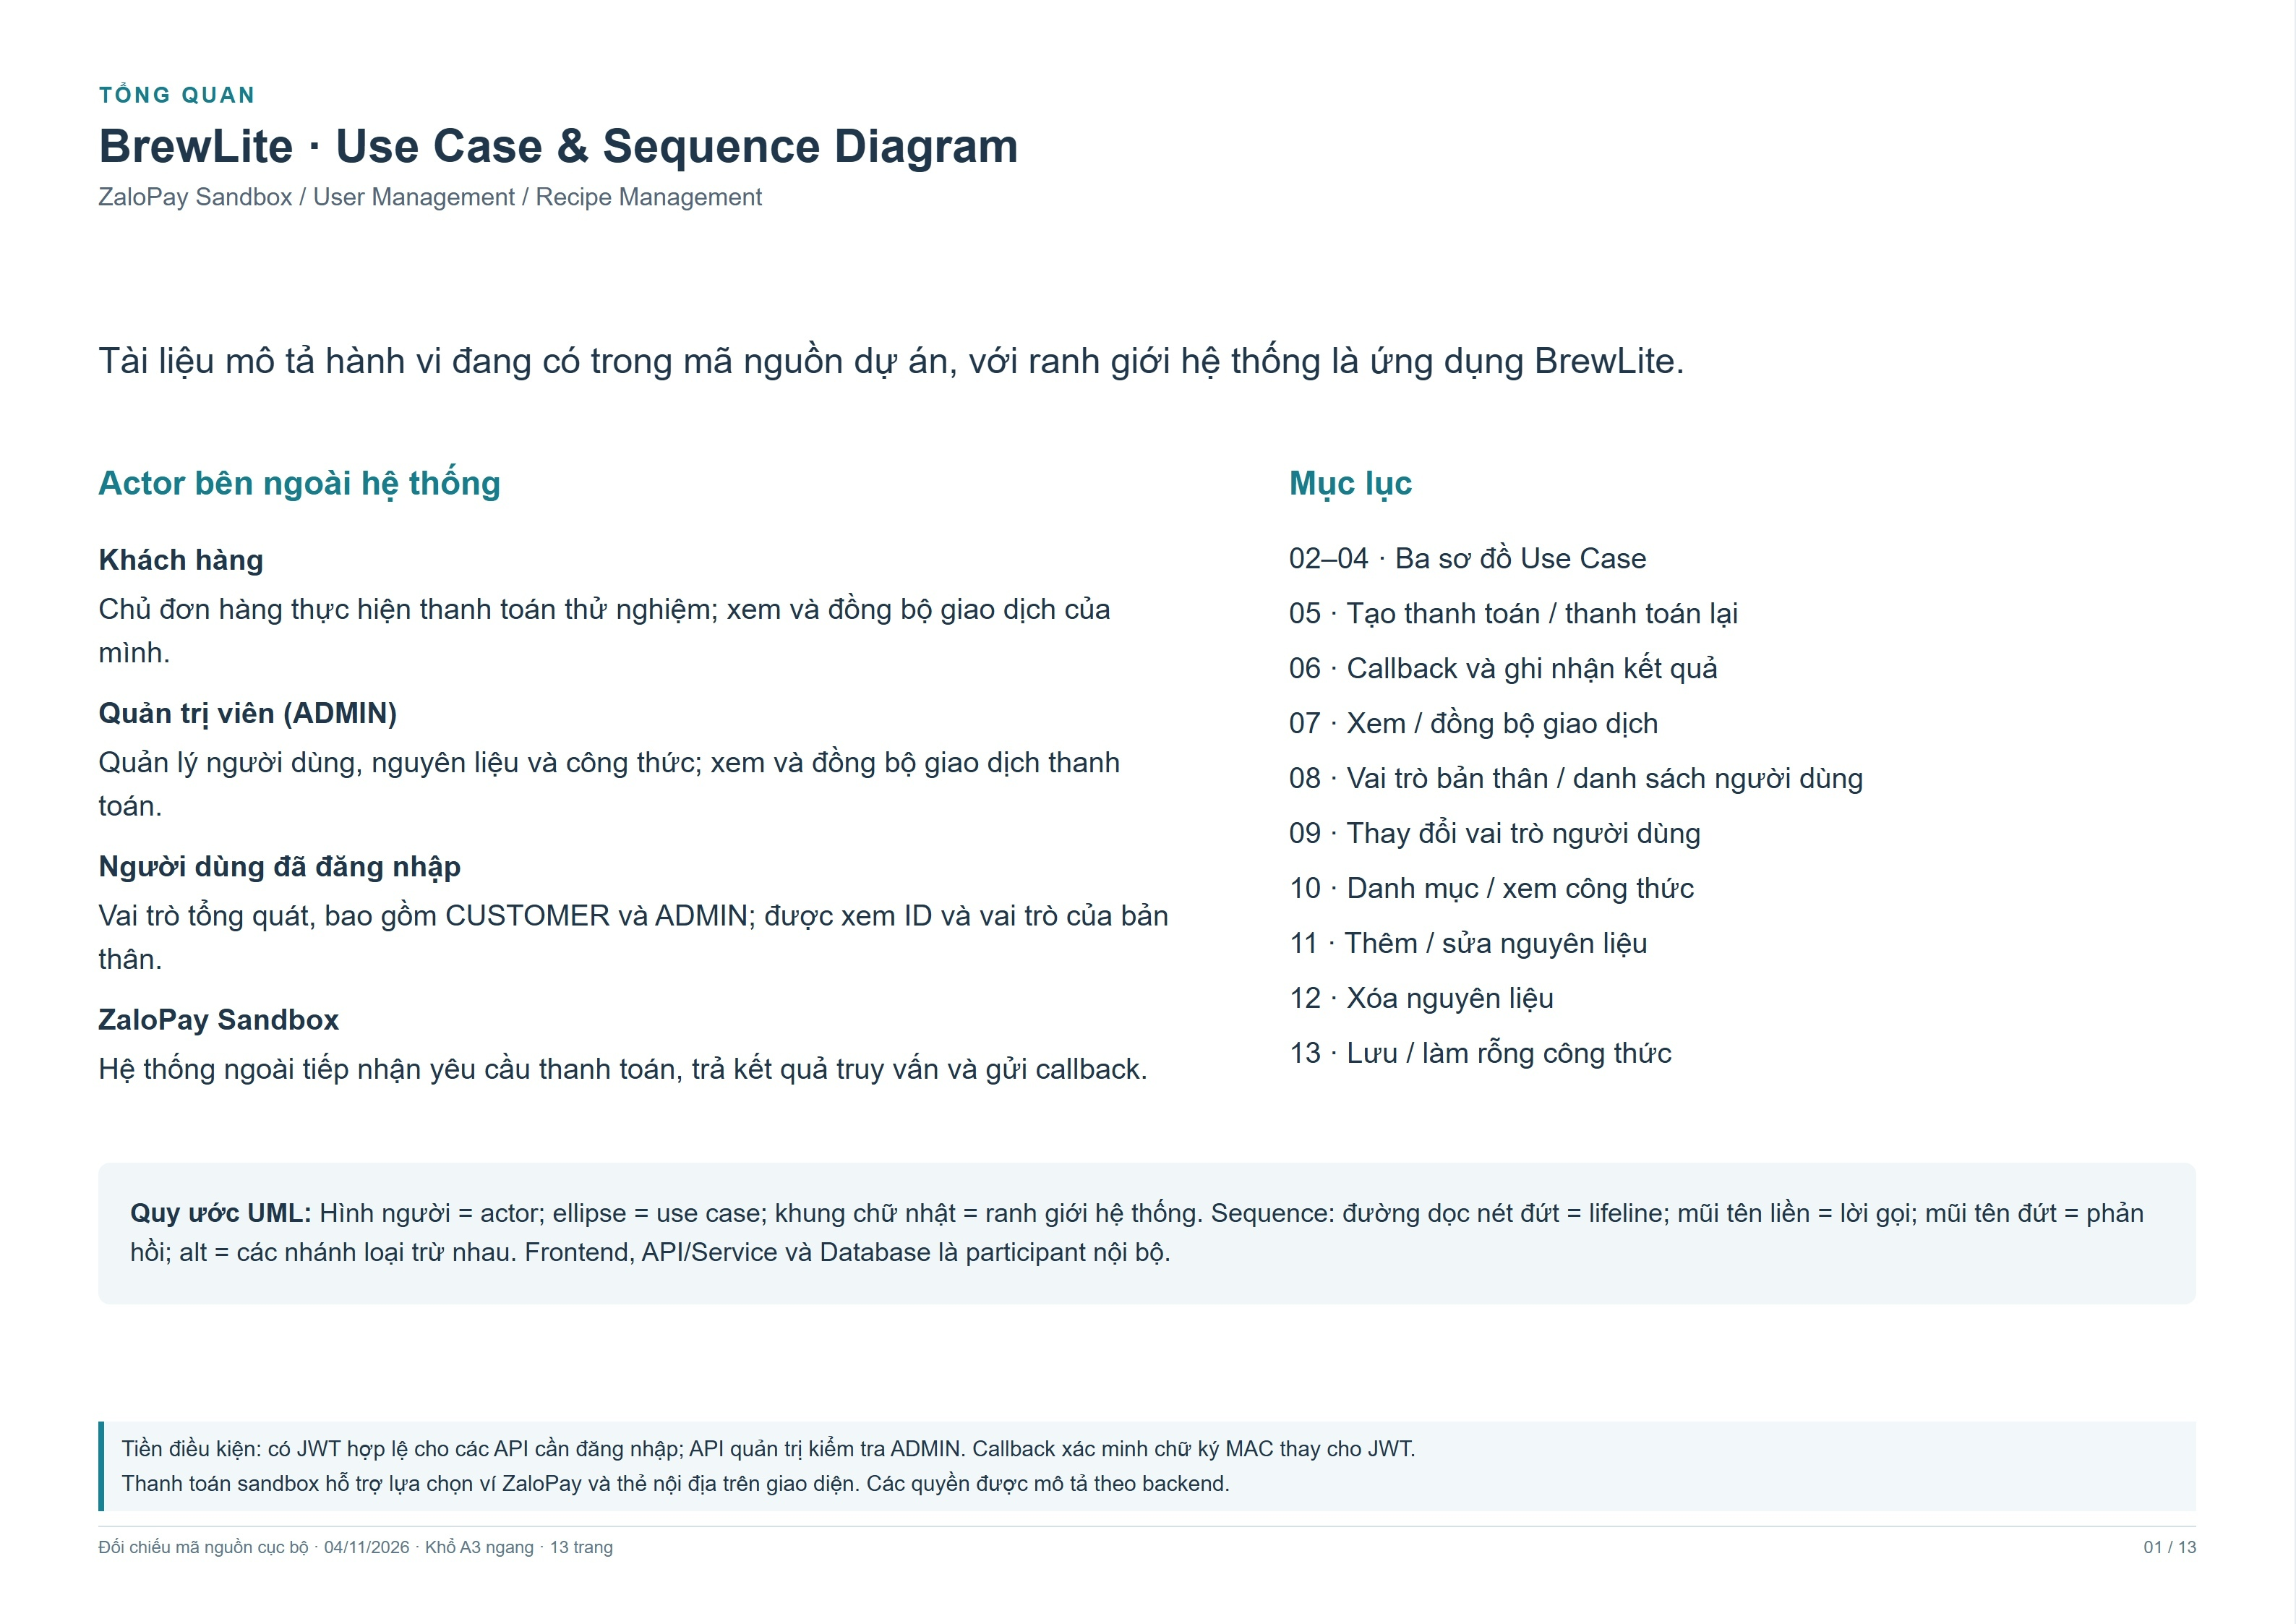
\includegraphics[width=\textwidth,height=0.45\textheight,keepaspectratio]{../figures/diagrams/overview-zalopay-users-recipes.png}
\caption{Tổng quan các phân hệ tương tác: ZaloPay Sandbox, Quản lý người dùng và Công thức định lượng}
\label{fig:overview-zalopay-users-recipes}
\end{figure}

Phân hệ bao gồm 3 tác nhân bên ngoài hệ thống tương tác qua API:
\begin{itemize}[leftmargin=1.5em]
  \item \textbf{Khách hàng (Chủ đơn):} Chủ đơn hàng thực hiện thanh toán thử nghiệm; xem và đồng bộ giao dịch thanh toán của chính mình.
  \item \textbf{Quản trị viên (ADMIN):} Xem và đồng bộ giao dịch của người khác; tuy nhiên, thao tác tạo thanh toán luôn yêu cầu tài khoản phải là chủ đơn (kể cả đối với tài khoản ADMIN).
  \item \textbf{ZaloPay Sandbox:} Hệ thống bên thứ ba tiếp nhận yêu cầu thanh toán, trả kết quả truy vấn trạng thái và gửi webhook callback.
\end{itemize}

\subsection{Sơ đồ Use Case: Cổng thanh toán ZaloPay Sandbox}

\begin{figure}[H]
\centering
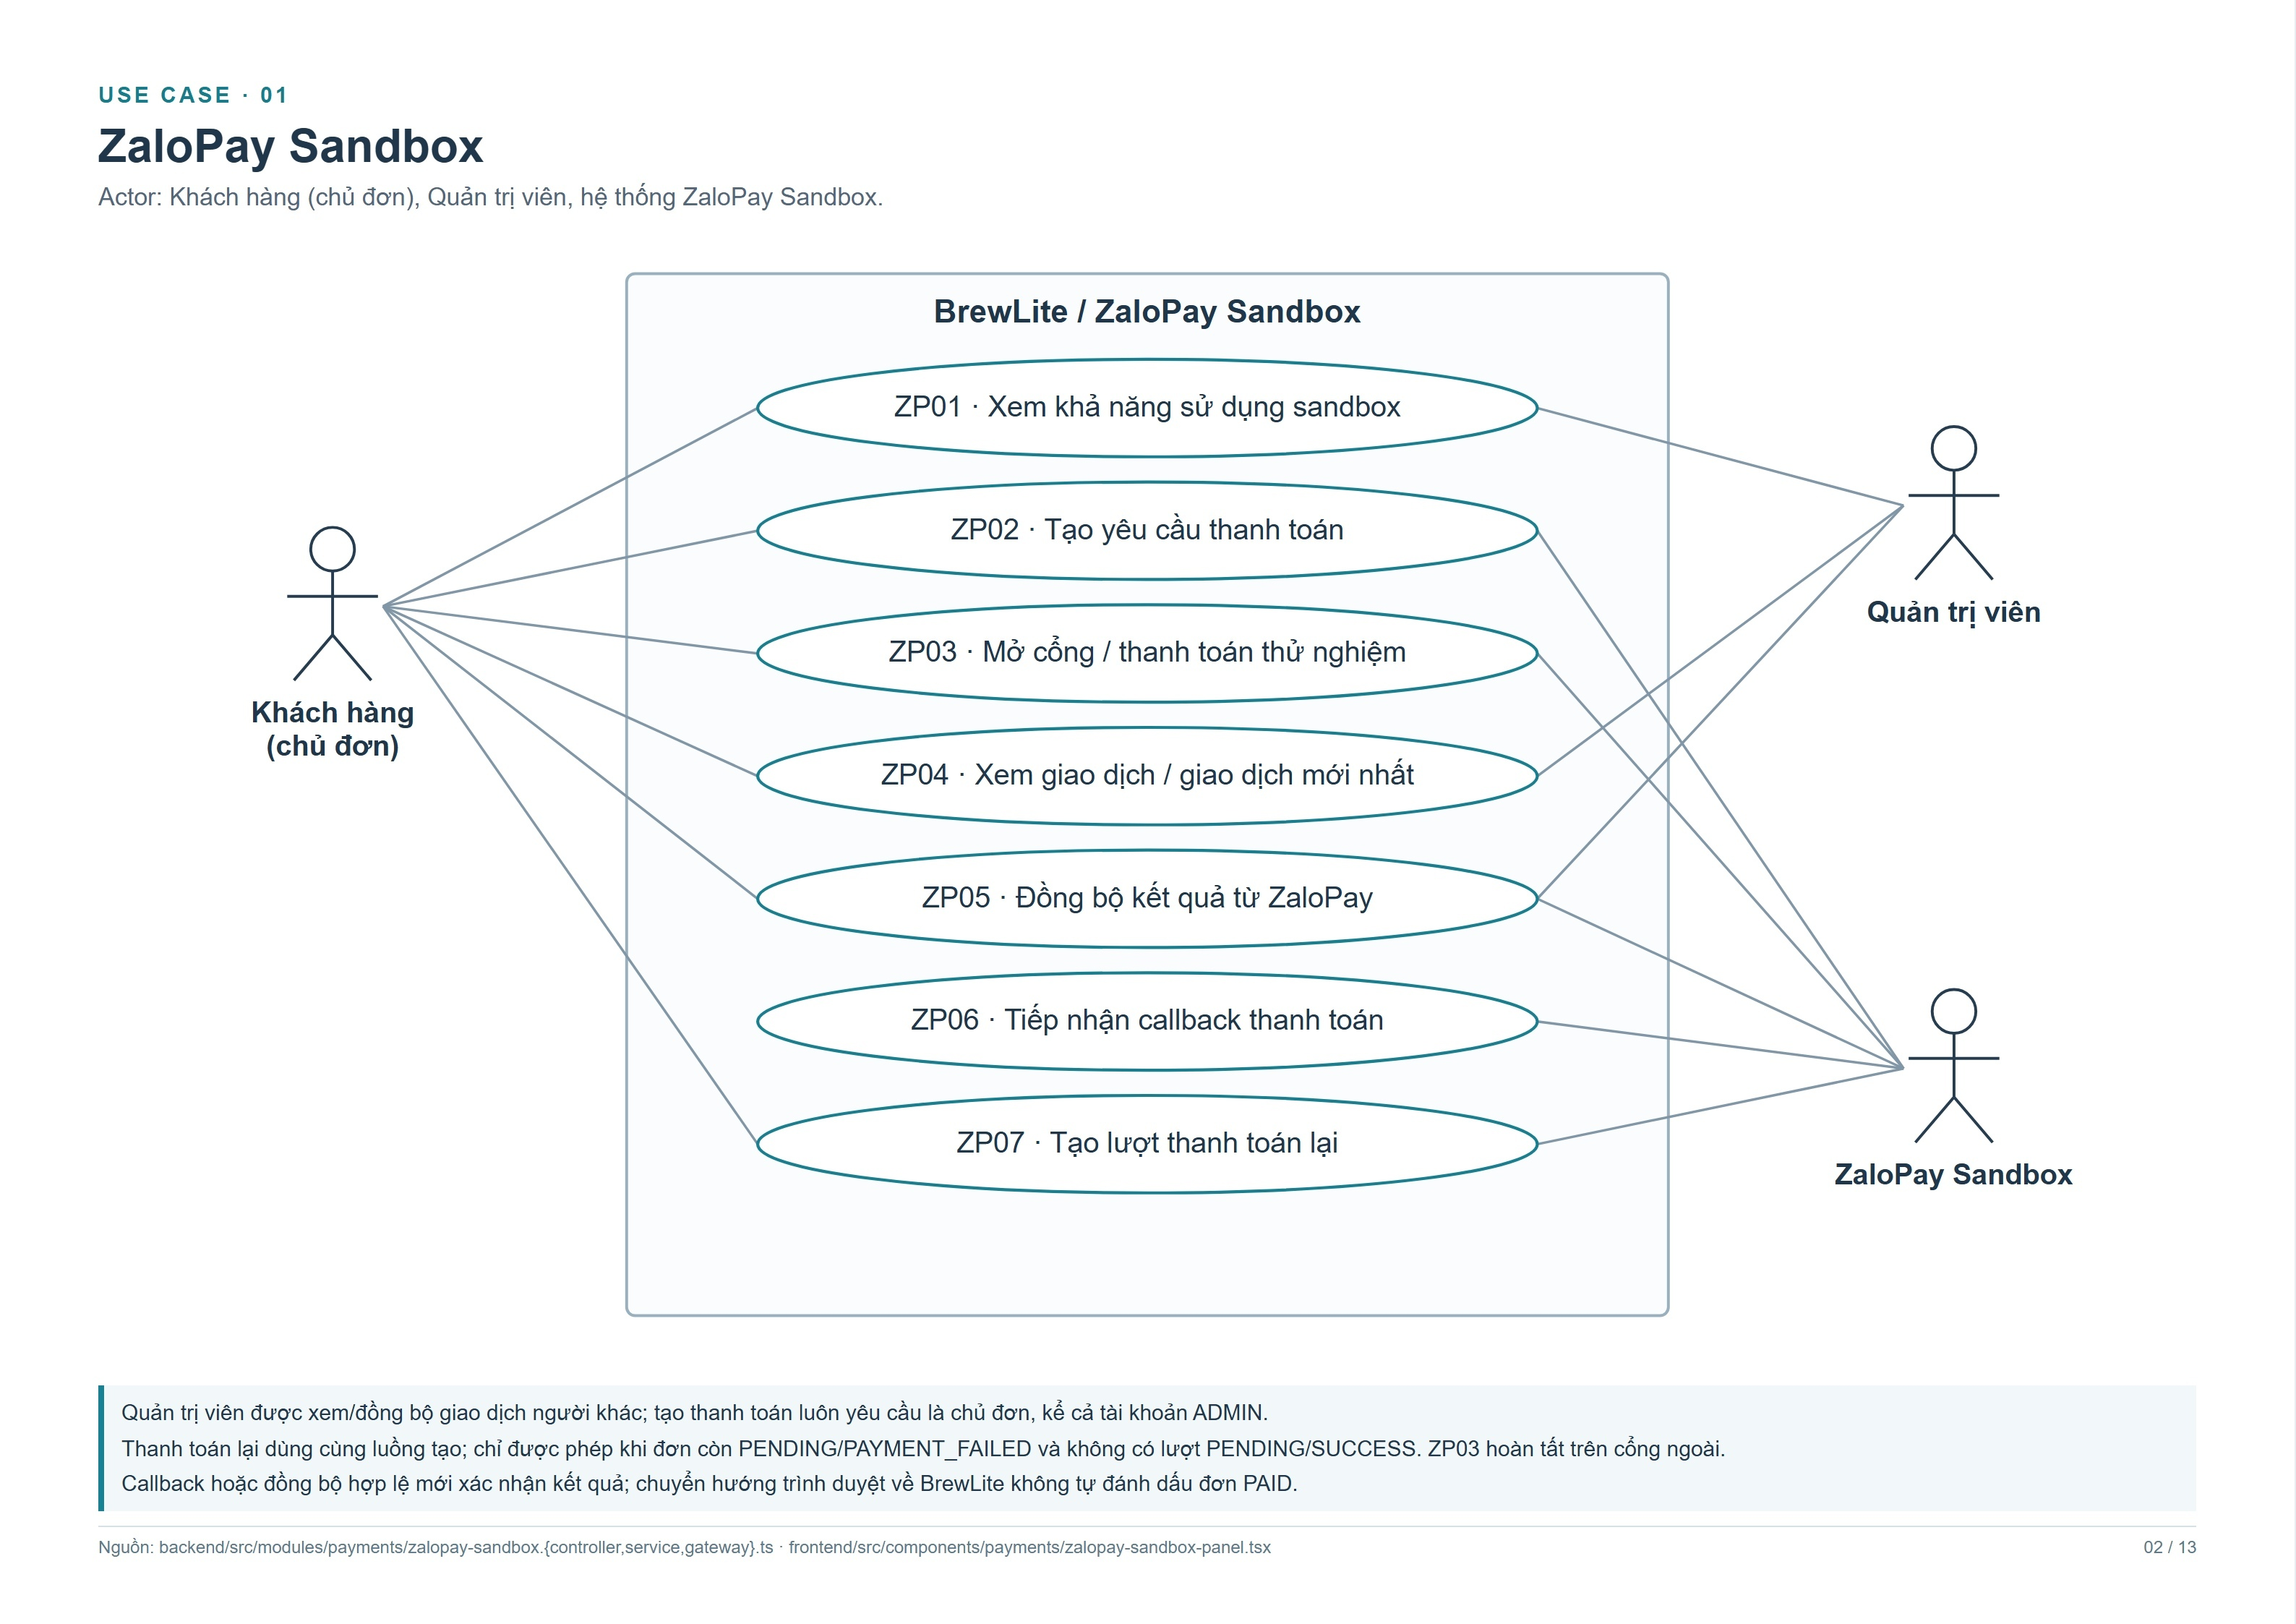
\includegraphics[width=\textwidth,height=0.45\textheight,keepaspectratio]{../figures/diagrams/uc-zalopay-sandbox-hd.png}
\caption{Use Case Diagram: Phân hệ ZaloPay Sandbox (ZP01 -- ZP07)}
\label{fig:uc-zalopay-sandbox}
\end{figure}

\begin{table}[H]
\centering\small
\caption{Danh mục Use Case phân hệ ZaloPay Sandbox}
\label{tab:uc-zalopay-list}
\begin{tabularx}{\textwidth}{@{}l p{4.5cm} X p{3.2cm}@{}}
\toprule
\textbf{Mã UC} & \textbf{Tên Use Case} & \textbf{Mô tả nghiệp vụ} & \textbf{Endpoint / Cơ chế} \\
\midrule
ZP01 & Xem khả năng sử dụng sandbox & Kiểm tra cổng thanh toán đã được bật cấu hình thử nghiệm chưa. & \code{GET /payments/zalopay/config} \\
ZP02 & Tạo yêu cầu thanh toán & Khởi tạo phiên thanh toán ví/thẻ, ký mã HMAC, sinh URL thanh toán. & \code{POST /payments/zalopay} \\
ZP03 & Mở cổng / thanh toán thử nghiệm & Khách hàng chuyển hướng sang cổng ZaloPay để quét QR hoặc nhập OTP. & Webview / External Host \\
ZP04 & Xem giao dịch mới nhất & Truy vấn lịch sử giao dịch thanh toán gần nhất theo đơn hàng. & \code{GET /payments/zalopay/:orderId} \\
ZP05 & Đồng bộ kết quả từ ZaloPay & Chủ động gọi API kiểm tra trạng thái giao dịch từ phía ZaloPay Server. & \code{POST /payments/zalopay/:id/sync} \\
ZP06 & Tiếp nhận callback thanh toán & Nhận thông báo IPN tự động từ ZaloPay khi thanh toán thành công. & \code{POST /payments/zalopay/callback} \\
ZP07 & Tạo lượt thanh toán lại & Kích hoạt thanh toán lại cho đơn \code{PENDING} hoặc \code{PAYMENT\_FAILED}. & \code{POST /payments/zalopay} (Replay) \\
\bottomrule
\end{tabularx}
\end{table}

\begin{note}[Quy tắc kiểm soát trạng thái thanh toán ZaloPay]
\begin{enumerate}[label=\alph*.]
  \item \textbf{Chống tạo trùng (Idempotency):} Mọi yêu cầu tạo thanh toán đều bắt buộc mang header \code{Idempotency-Key}. Nếu gửi lặp cùng key và cùng nội dung, hệ thống trả lại giao dịch cũ mà không gọi lại mạng sang ZaloPay.
  \item \textbf{Không tự động đánh dấu PAID khi redirect:} Việc chuyển hướng trình duyệt từ ZaloPay quay về trang web BrewLite tuyệt đối không tự đánh dấu đơn là \code{PAID}. Chỉ có Callback hợp lệ mang chữ ký MAC đúng (\code{ZP06}) hoặc thao tác đồng bộ máy chủ (\code{ZP05}) mới có thẩm quyền chuyển trạng thái đơn.
  \item \textbf{Thăm dò cục bộ an toàn:} Giao diện Frontend tự động thăm dò đọc lại dữ liệu mỗi 15 giây khi đang chờ, nhưng thao tác này chỉ đọc database nội bộ của BrewLite, không gửi truy vấn sang ZaloPay để bảo vệ hạn ngạch rate limit.
\end{enumerate}
\end{note}

\subsection{Các sơ đồ tuần tự chi tiết của phân hệ ZaloPay}

\subsubsection{Sequence: Tạo thanh toán và thanh toán lại (ZP02, ZP03, ZP07)}
Sơ đồ thể hiện quy trình tạo phiên thanh toán mới kèm bảo vệ chống lặp qua \code{Idempotency-Key}, xác thực quyền chủ đơn, ghi nhận bản ghi \code{Payment} trạng thái \code{PENDING} trước khi gọi ra cổng ngoài và xử lý phân nhánh kết quả từ ZaloPay Sandbox:

\begin{figure}[H]
\centering
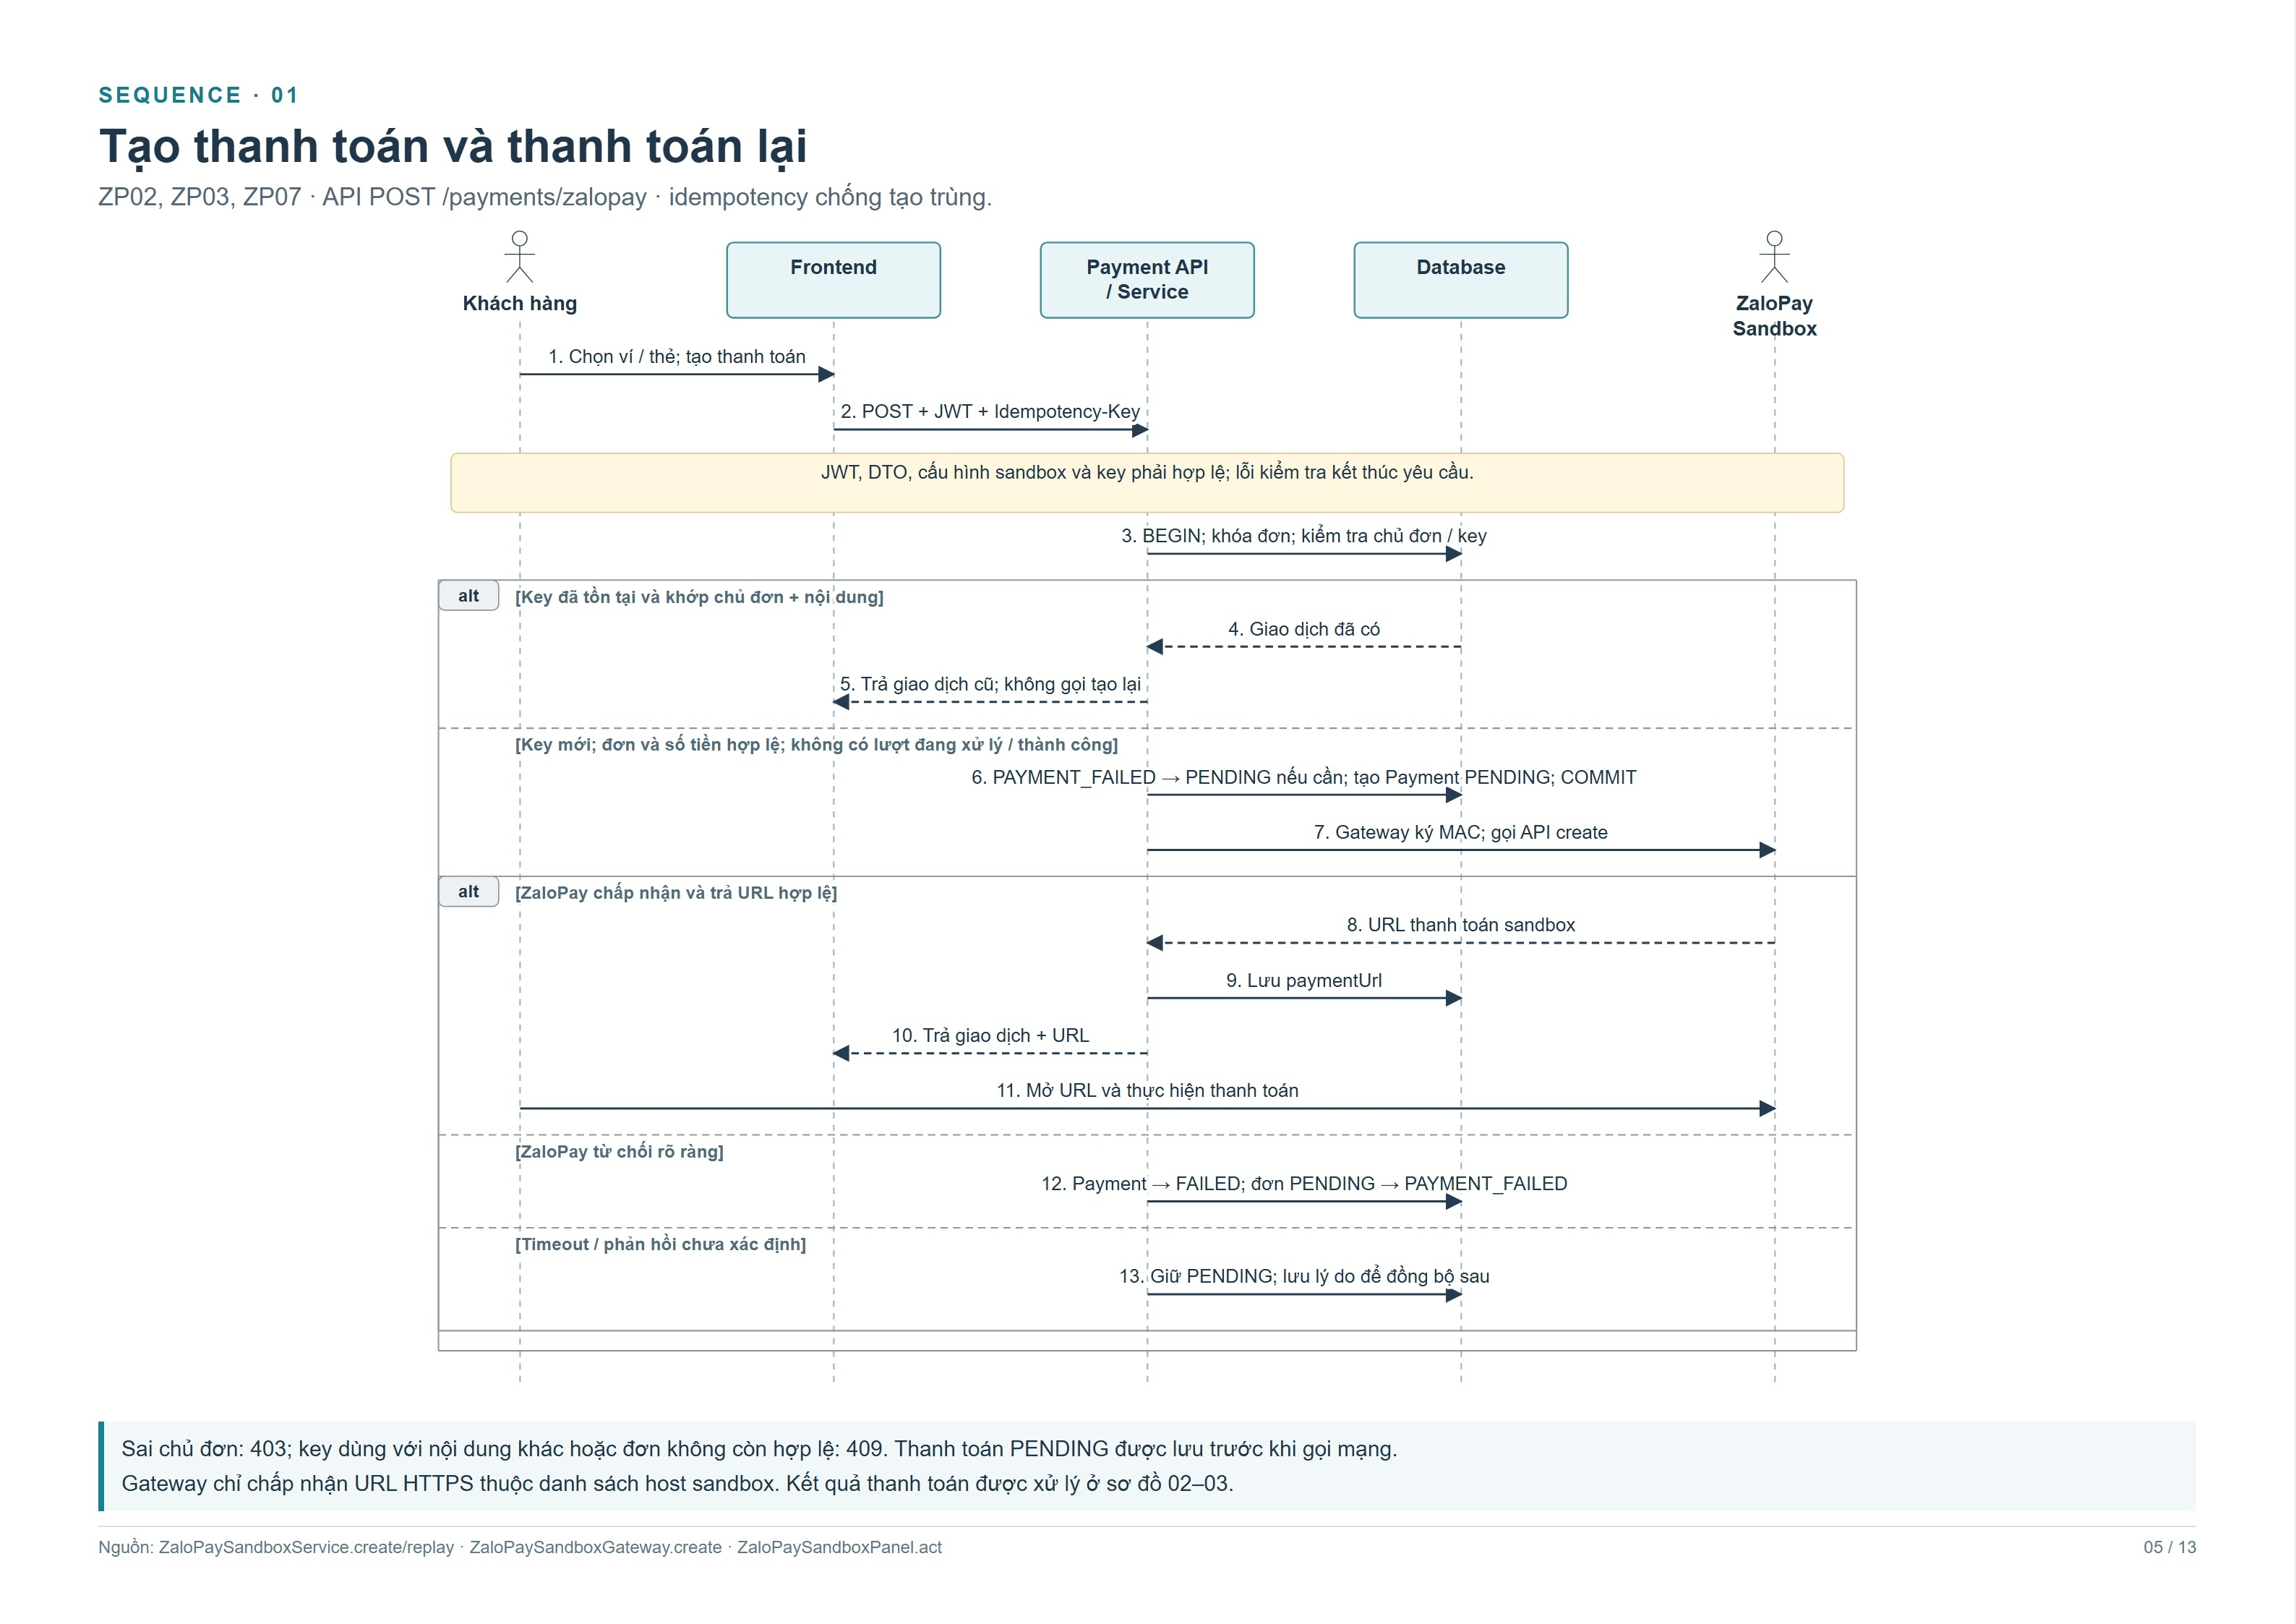
\includegraphics[width=\textwidth,height=0.48\textheight,keepaspectratio]{../figures/diagrams/sd-zalopay-create-hd.png}
\caption{Sequence Diagram: Tạo thanh toán và thanh toán lại (ZP02, ZP03, ZP07)}
\label{fig:sd-zalopay-create}
\end{figure}

\subsubsection{Sequence: Callback và ghi nhận thanh toán (ZP06)}
Sơ đồ mô tả quy trình tiếp nhận IPN Callback từ ZaloPay: xác thực chữ ký điện tử HMAC-SHA256, đối soát mã giao dịch và số tiền trong Transaction ACID, cập nhật trạng thái đơn hàng sang \code{PAID} và ghi nhận lý do đối soát (\code{reviewReason}) nếu phát hiện sai lệch số tiền:

\begin{figure}[H]
\centering
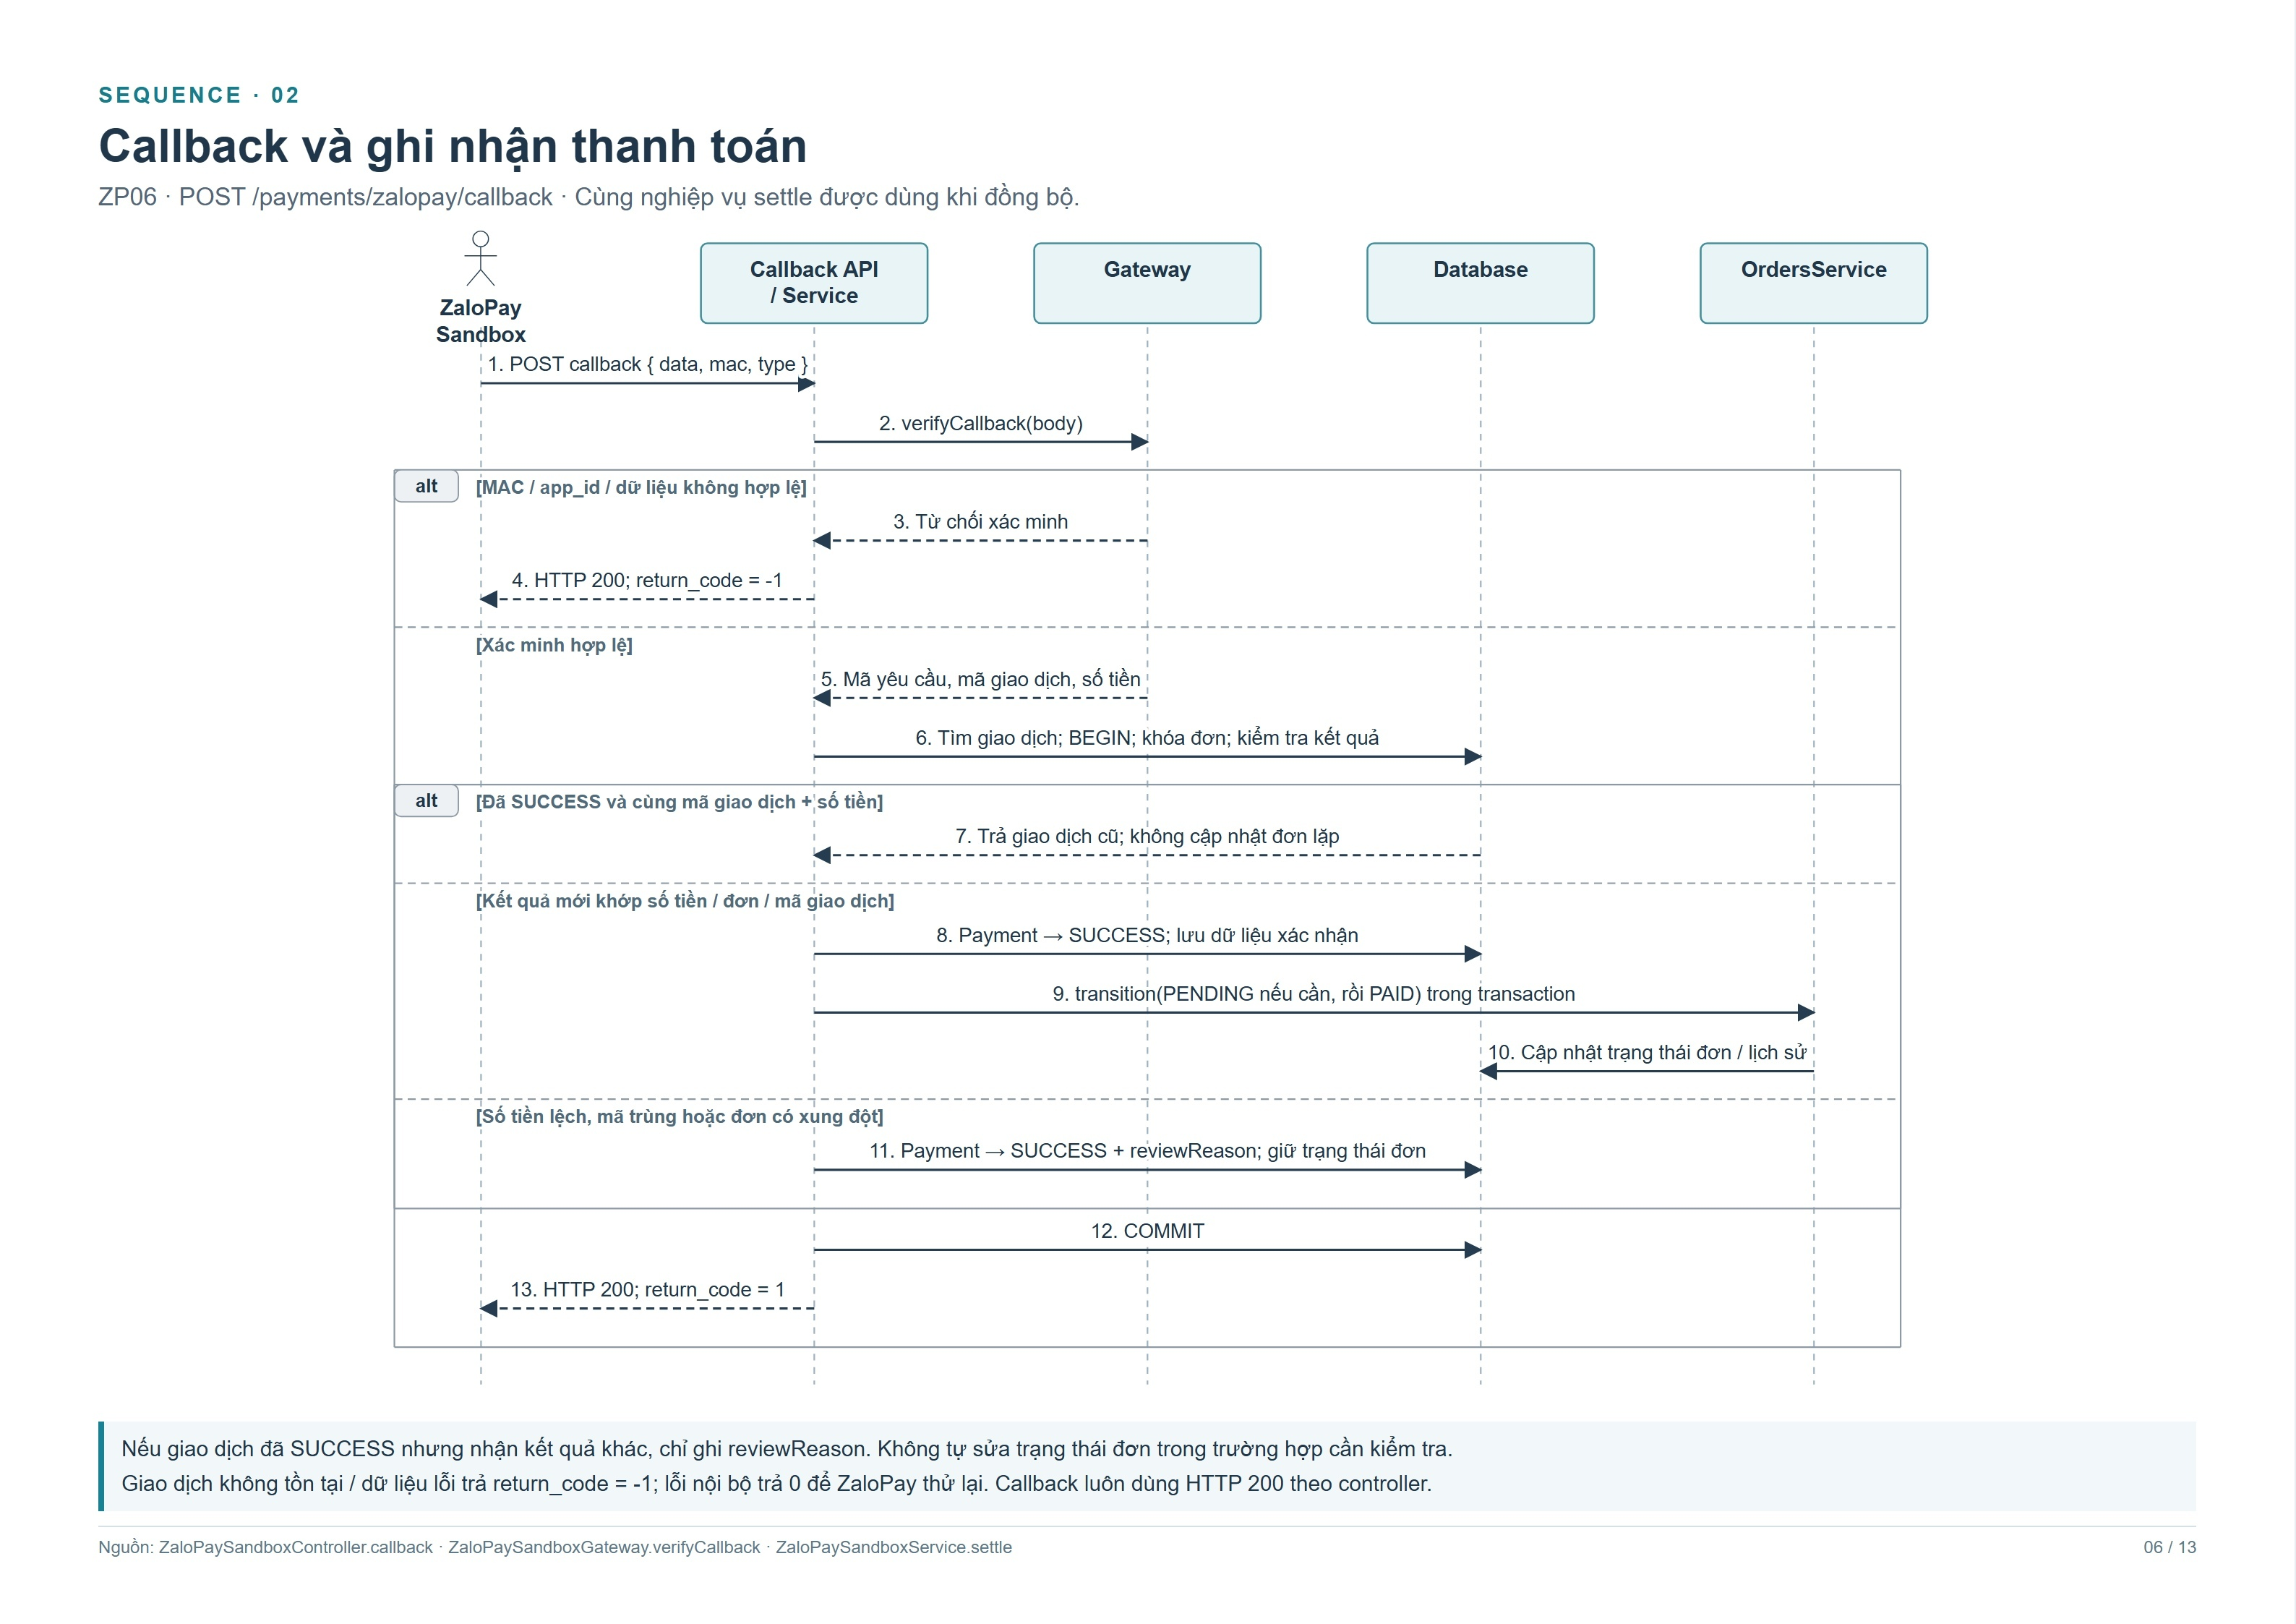
\includegraphics[width=\textwidth,height=0.48\textheight,keepaspectratio]{../figures/diagrams/sd-zalopay-callback-hd.png}
\caption{Sequence Diagram: Tiếp nhận Callback và ghi nhận thanh toán (ZP06)}
\label{fig:sd-zalopay-callback}
\end{figure}

\subsubsection{Sequence: Xem và đồng bộ giao dịch (ZP01, ZP04, ZP05)}
Sơ đồ thể hiện luồng chủ động đối soát trạng thái giao dịch giữa BrewLite và ZaloPay Gateway khi khách hàng bấm nút ``Kiểm tra kết quả'' hoặc hệ thống cần xác định trạng thái cuối của một giao dịch đang treo:

\begin{figure}[H]
\centering
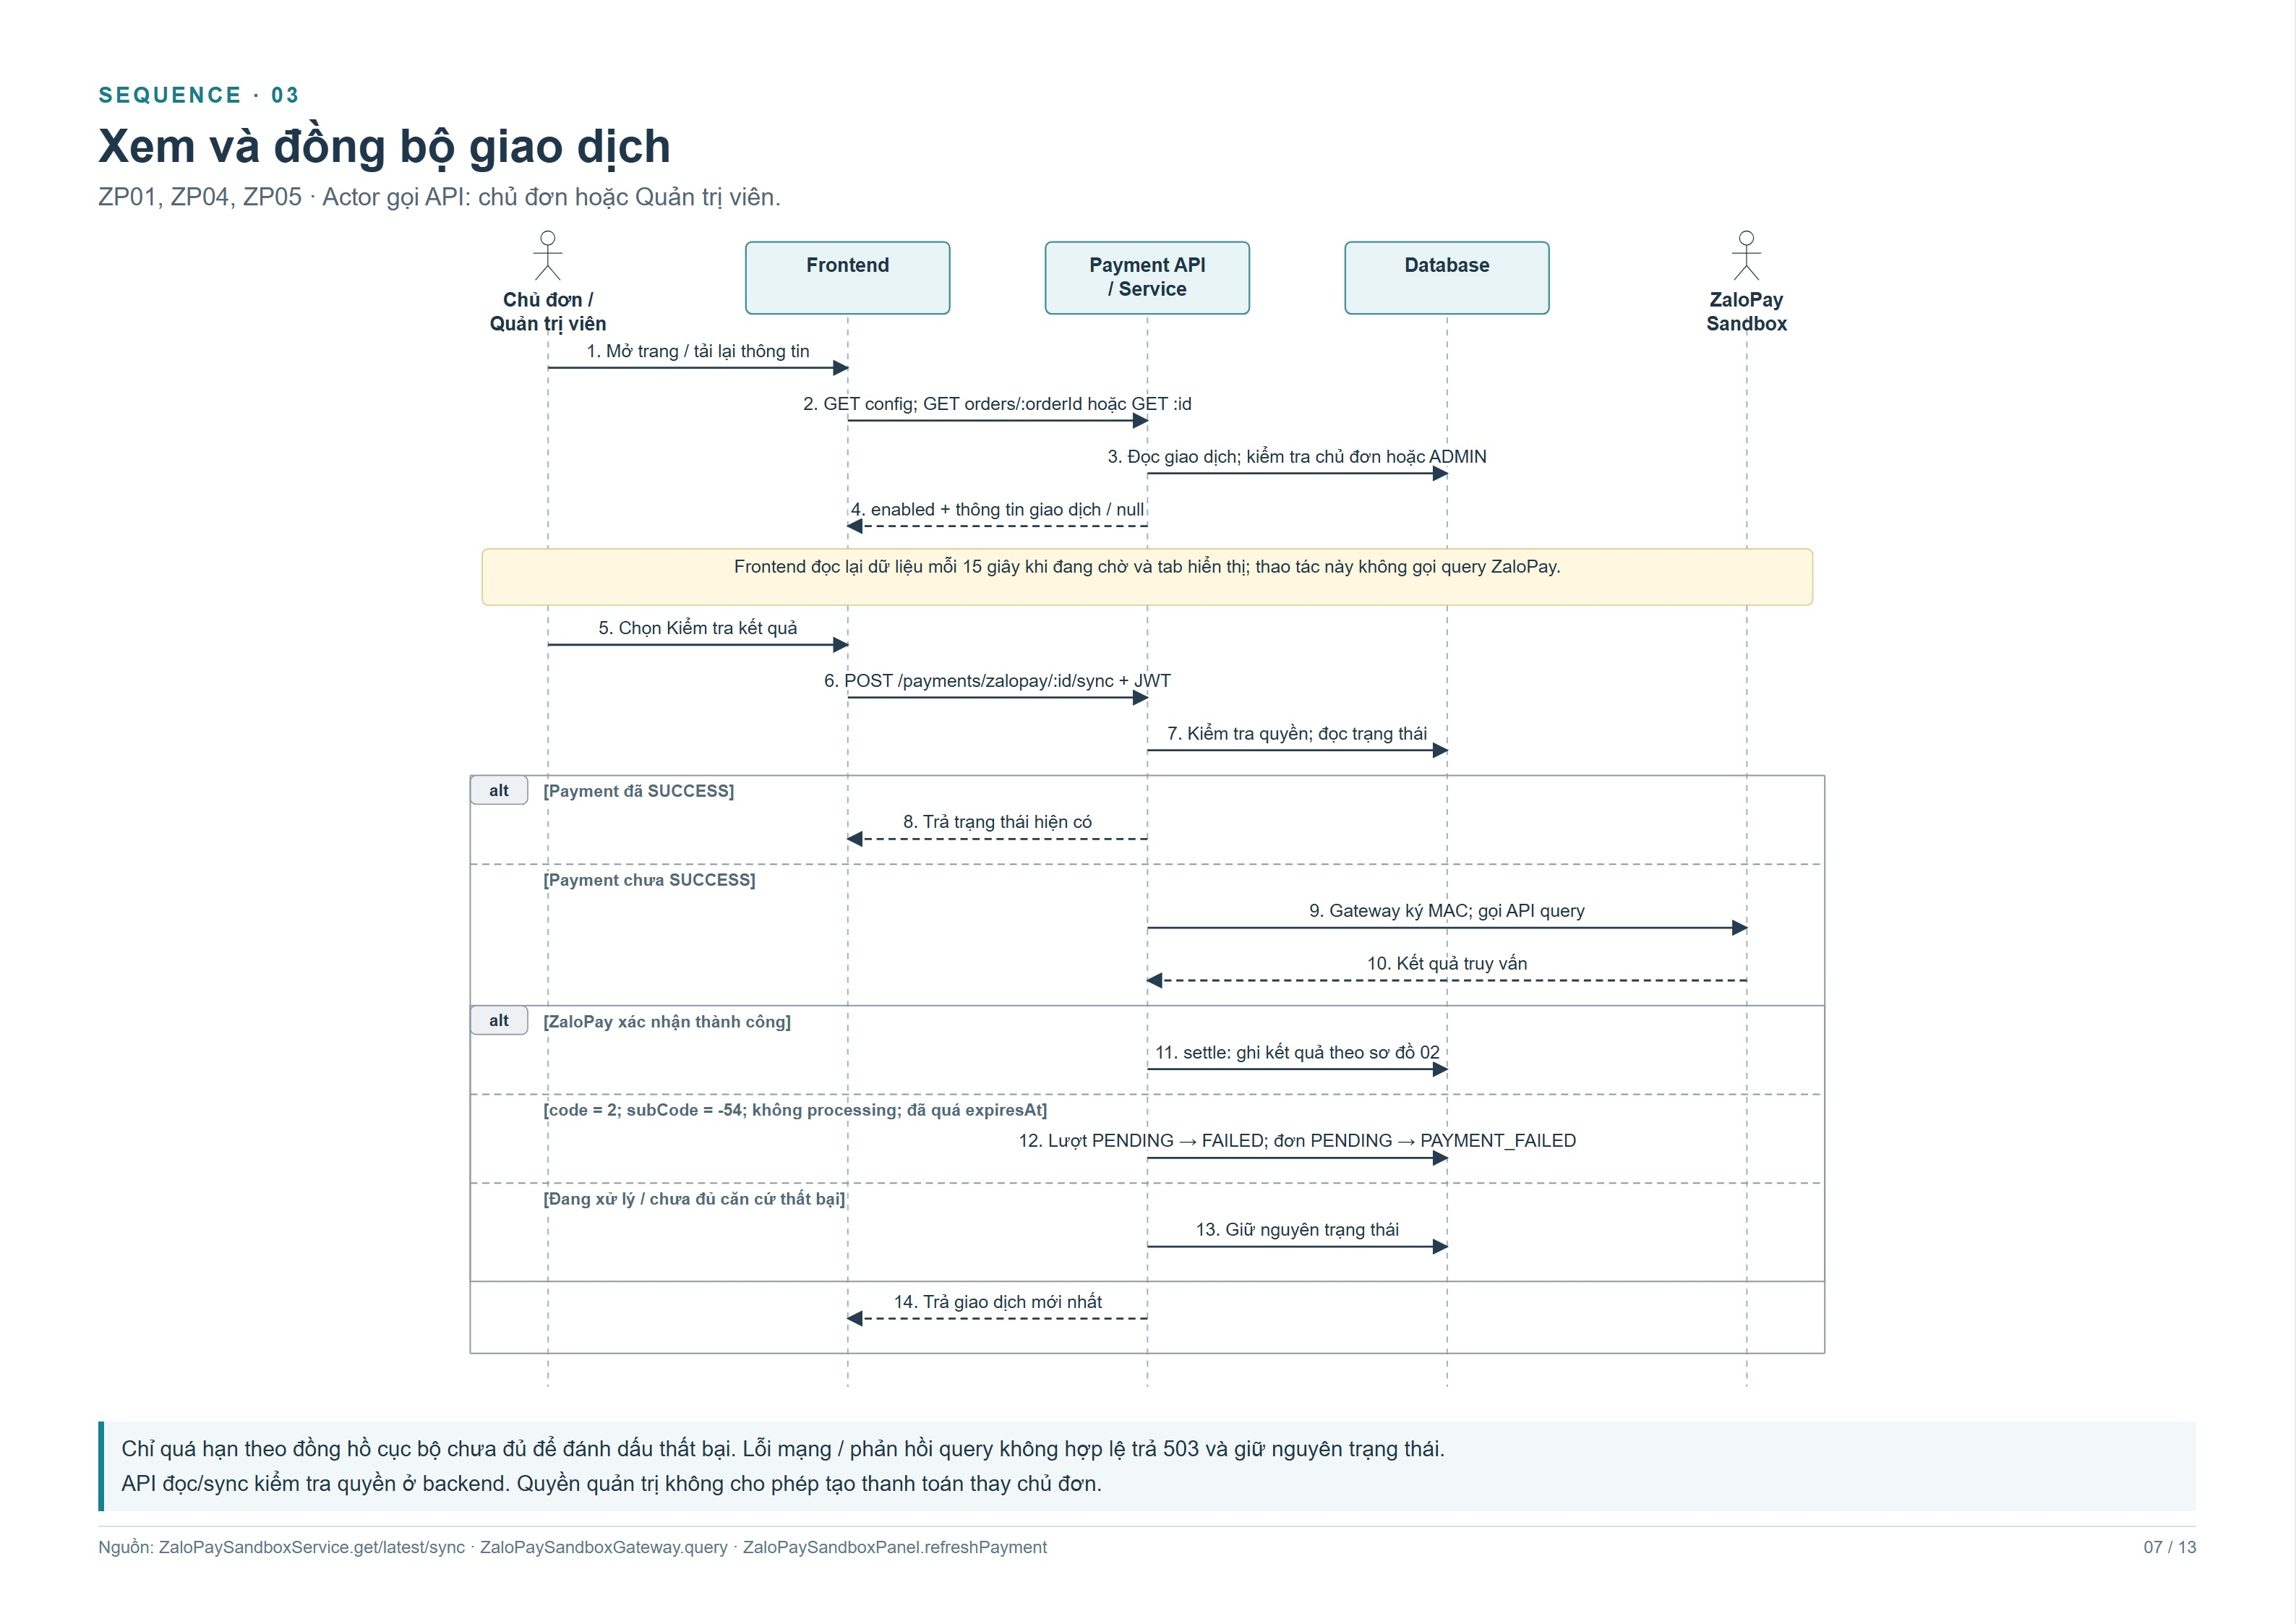
\includegraphics[width=\textwidth,height=0.48\textheight,keepaspectratio]{../figures/diagrams/sd-zalopay-sync-hd.png}
\caption{Sequence Diagram: Xem và đồng bộ giao dịch (ZP01, ZP04, ZP05)}
\label{fig:sd-zalopay-sync}
\end{figure}

% =====================================================================
%  Phụ lục G: Phân hệ Quản lý người dùng và phân quyền (User Management)
%  Nguồn: backend/src/modules/users/*, admin.guard.ts
% =====================================================================
\section{Phân hệ Quản lý người dùng và phân quyền (User Management Module)}
\label{app:user-mgmt}

Phân hệ quản lý thông tin danh tính, phân vai trò người dùng (Role-Based Access Control) và các chính sách bảo mật chống leo thang đặc quyền trong hệ thống BrewLite.

\subsection{Sơ đồ Use Case: Quản lý người dùng}

\begin{figure}[H]
\centering
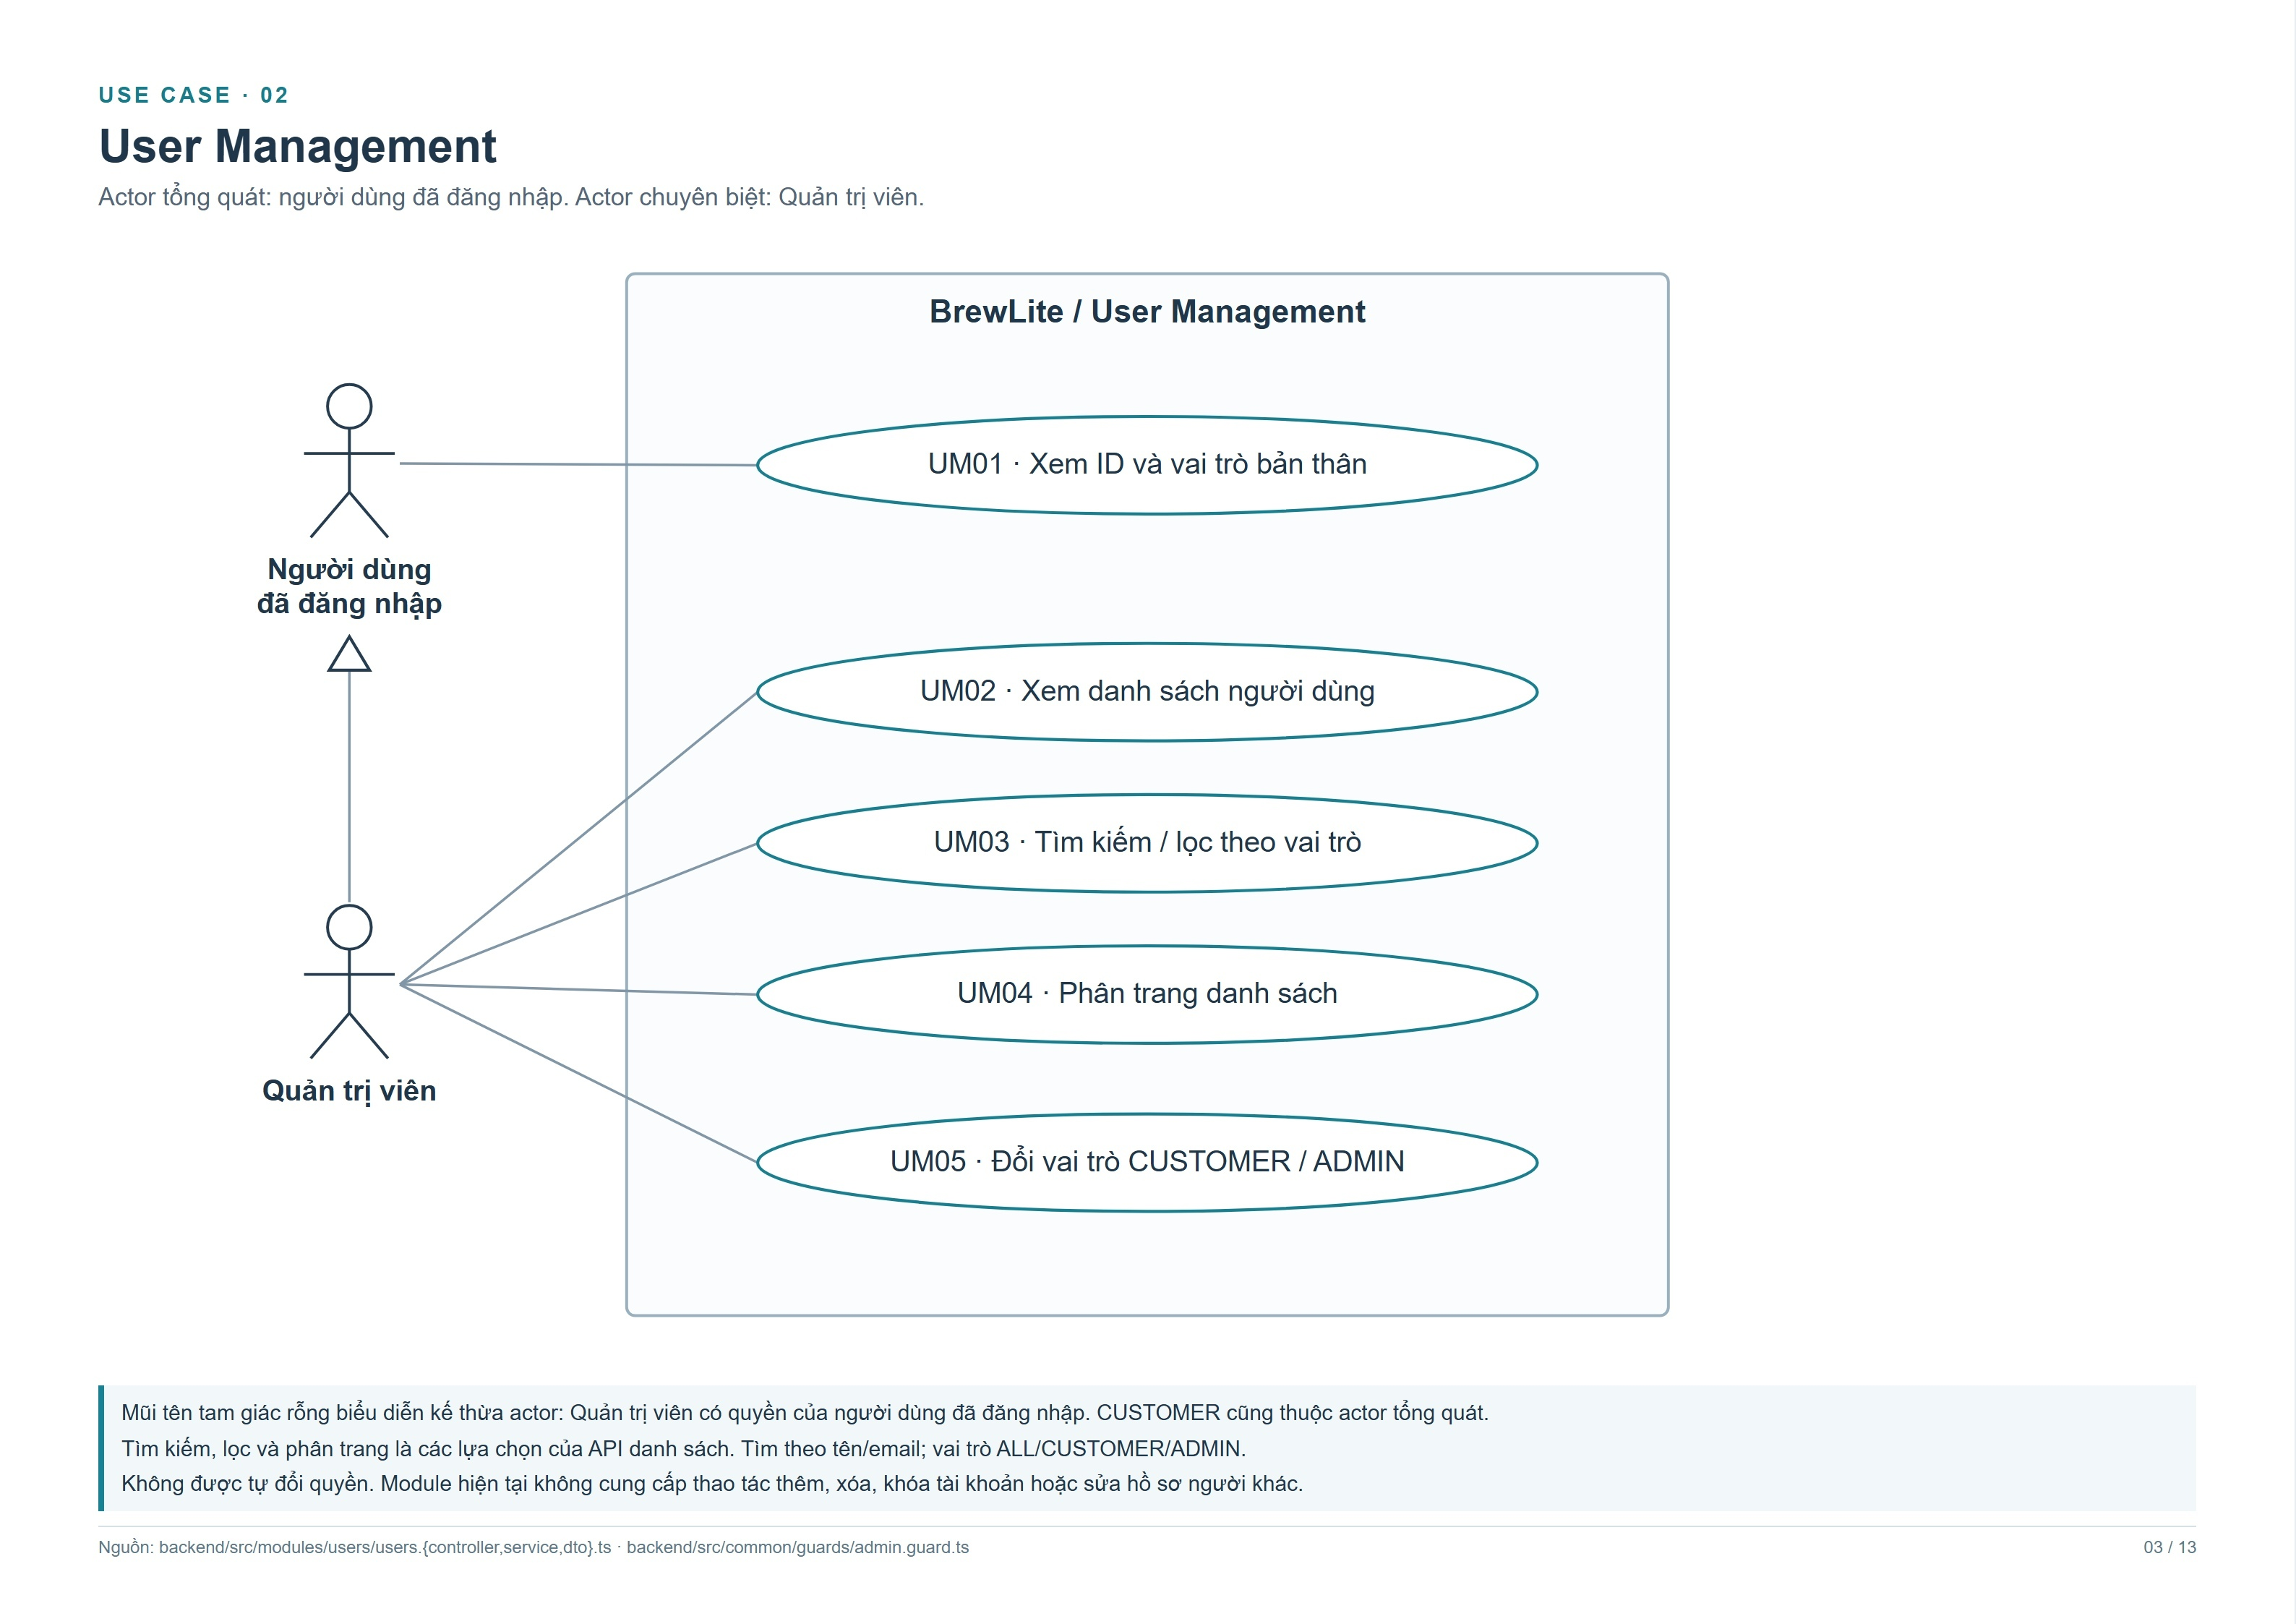
\includegraphics[width=\textwidth,height=0.45\textheight,keepaspectratio]{../figures/diagrams/uc-user-mgmt-hd.png}
\caption{Use Case Diagram: Phân hệ Quản lý người dùng (UM01 -- UM05)}
\label{fig:uc-user-mgmt}
\end{figure}

\begin{table}[H]
\centering\small
\caption{Danh mục Use Case phân hệ Quản lý người dùng}
\label{tab:uc-user-list}
\begin{tabularx}{\textwidth}{@{}l p{4.2cm} X p{3.5cm}@{}}
\toprule
\textbf{Mã UC} & \textbf{Tên Use Case} & \textbf{Mô tả nghiệp vụ} & \textbf{Actor \& Guard} \\
\midrule
UM01 & Xem ID và vai trò bản thân & Lấy thông tin ID, email và quyền hạn thực tế đang có trong phiên đăng nhập. & Người dùng đã đăng nhập (\code{JwtAuthGuard}) \\
UM02 & Xem danh sách người dùng & Hiển thị danh sách tài khoản thành viên trong hệ thống kèm số đơn đã đặt. & Quản trị viên (\code{AdminGuard}) \\
UM03 & Tìm kiếm / lọc theo vai trò & Tìm kiếm tài khoản theo tên, email (không dấu) và lọc theo nhóm vai trò. & Quản trị viên (\code{AdminGuard}) \\
UM04 & Phân trang danh sách & Duyệt danh sách theo trang (mặc định 10 dòng/trang, tối đa 50 dòng/trang). & Quản trị viên (\code{AdminGuard}) \\
UM05 & Đổi vai trò CUSTOMER / ADMIN & Nâng cấp hoặc thu hồi quyền quản trị viên của một tài khoản khác. & Quản trị viên (\code{AdminGuard}) \\
\bottomrule
\end{tabularx}
\end{table}

\begin{note}[Quy tắc an toàn phân quyền trong mã nguồn]
\begin{enumerate}[label=\alph*.]
  \item \textbf{Cấm tự thay đổi quyền của chính mình:} Hệ thống chặn đứng yêu cầu nếu \code{actorId == targetId} (trả mã lỗi HTTP 400 Bad Request), ngăn chặn tình huống vô tình khóa mất tài khoản Admin đang vận hành.
  \item \textbf{Tuần tự hóa giao dịch bằng Advisory Lock:} Khi thực hiện đổi quyền tài khoản, \code{UsersService} sử dụng cơ chế khóa cố vấn PostgreSQL (\code{pg\_advisory\_xact\_lock}) và kiểm tra lại vai trò của người thực hiện trong chính Transaction đó. Cơ chế này loại bỏ hoàn toàn khả năng hai quản trị viên đồng thời gửi yêu cầu hạ quyền nhau gây xung đột dữ liệu.
\end{enumerate}
\end{note}

\subsection{Các sơ đồ tuần tự chi tiết của phân hệ Người dùng}

\subsubsection{Sequence: Truy vấn vai trò bản thân và danh sách người dùng (UM01 -- UM04)}
Sơ đồ phân định rõ nhánh cho người dùng thường xem thông tin hồ sơ của chính mình qua \code{/admin/users/me} và nhánh cho Quản trị viên xem danh sách thành viên với cơ chế phân trang và tìm kiếm chạy trong transaction mức \code{RepeatableRead}:

\begin{figure}[H]
\centering
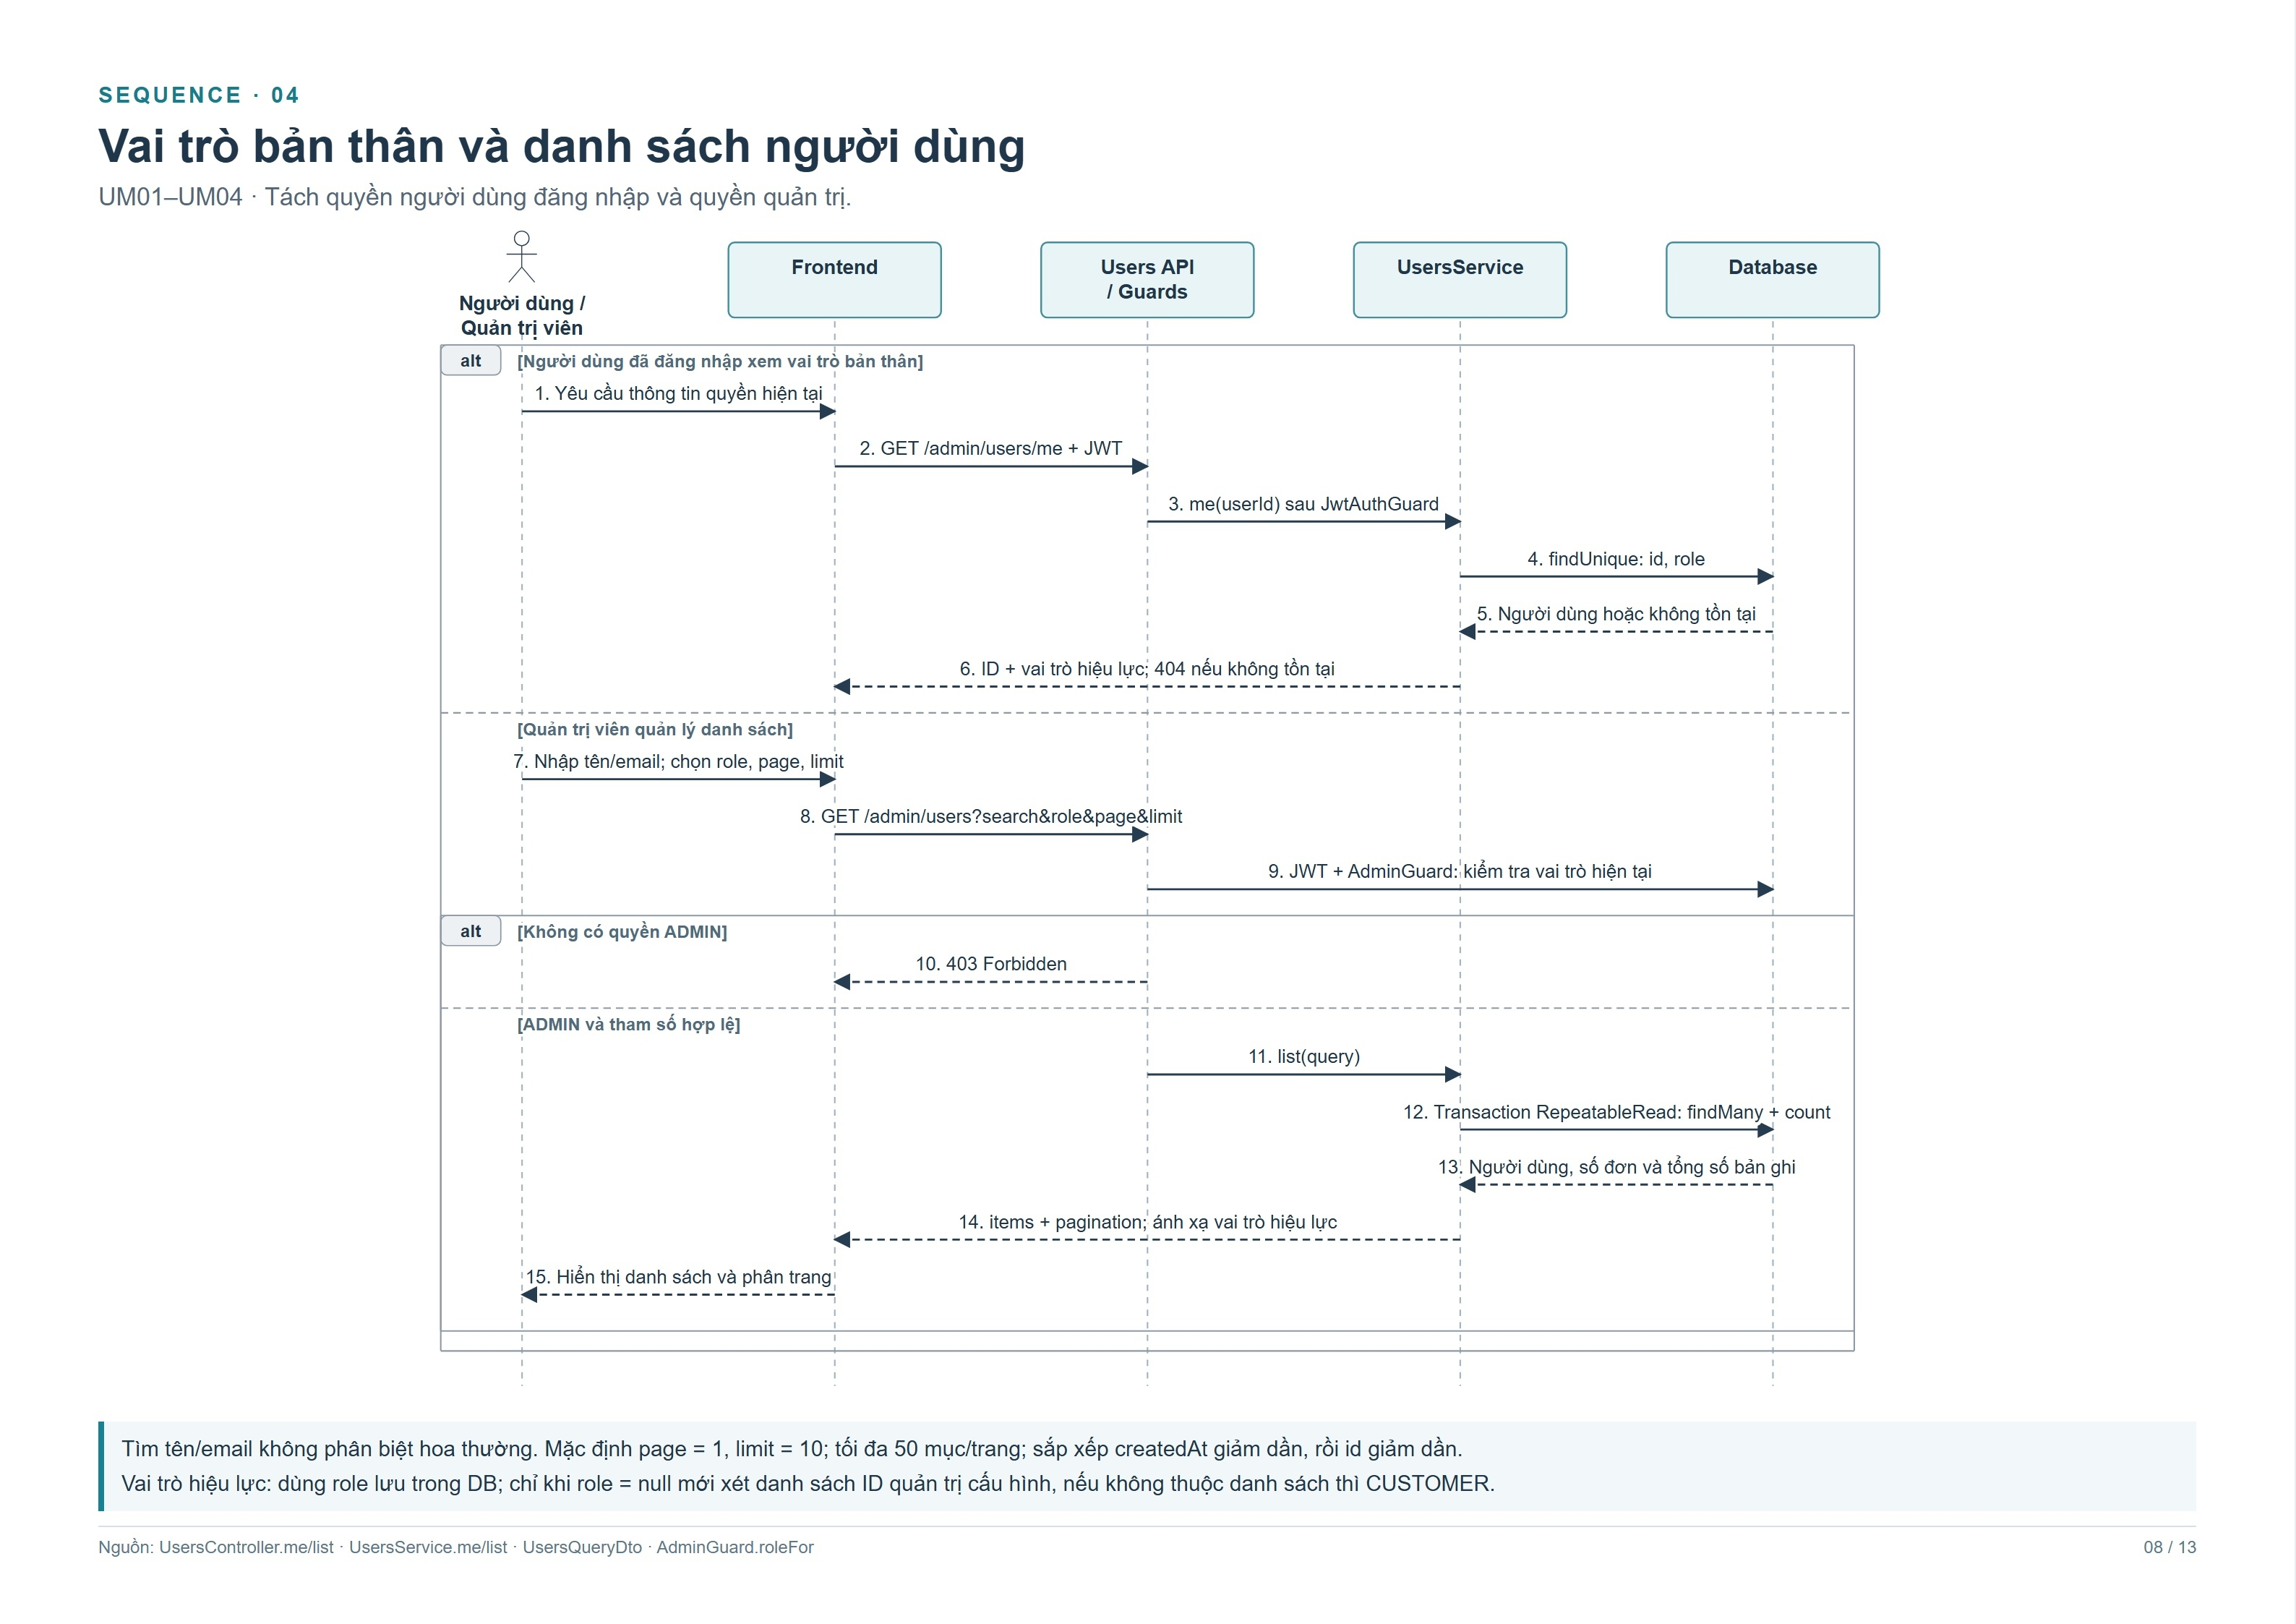
\includegraphics[width=\textwidth,height=0.48\textheight,keepaspectratio]{../figures/diagrams/sd-user-me-list-hd.png}
\caption{Sequence Diagram: Xem vai trò bản thân và quản lý danh sách người dùng (UM01 -- UM04)}
\label{fig:sd-user-me-list}
\end{figure}

\subsubsection{Sequence: Thay đổi vai trò người dùng (UM05)}
Sơ đồ thể hiện quy trình phân quyền an toàn, kiểm tra tự đổi quyền, áp dụng Advisory Lock trong transaction và các nhánh ngoại lệ bảo mật:

\begin{figure}[H]
\centering
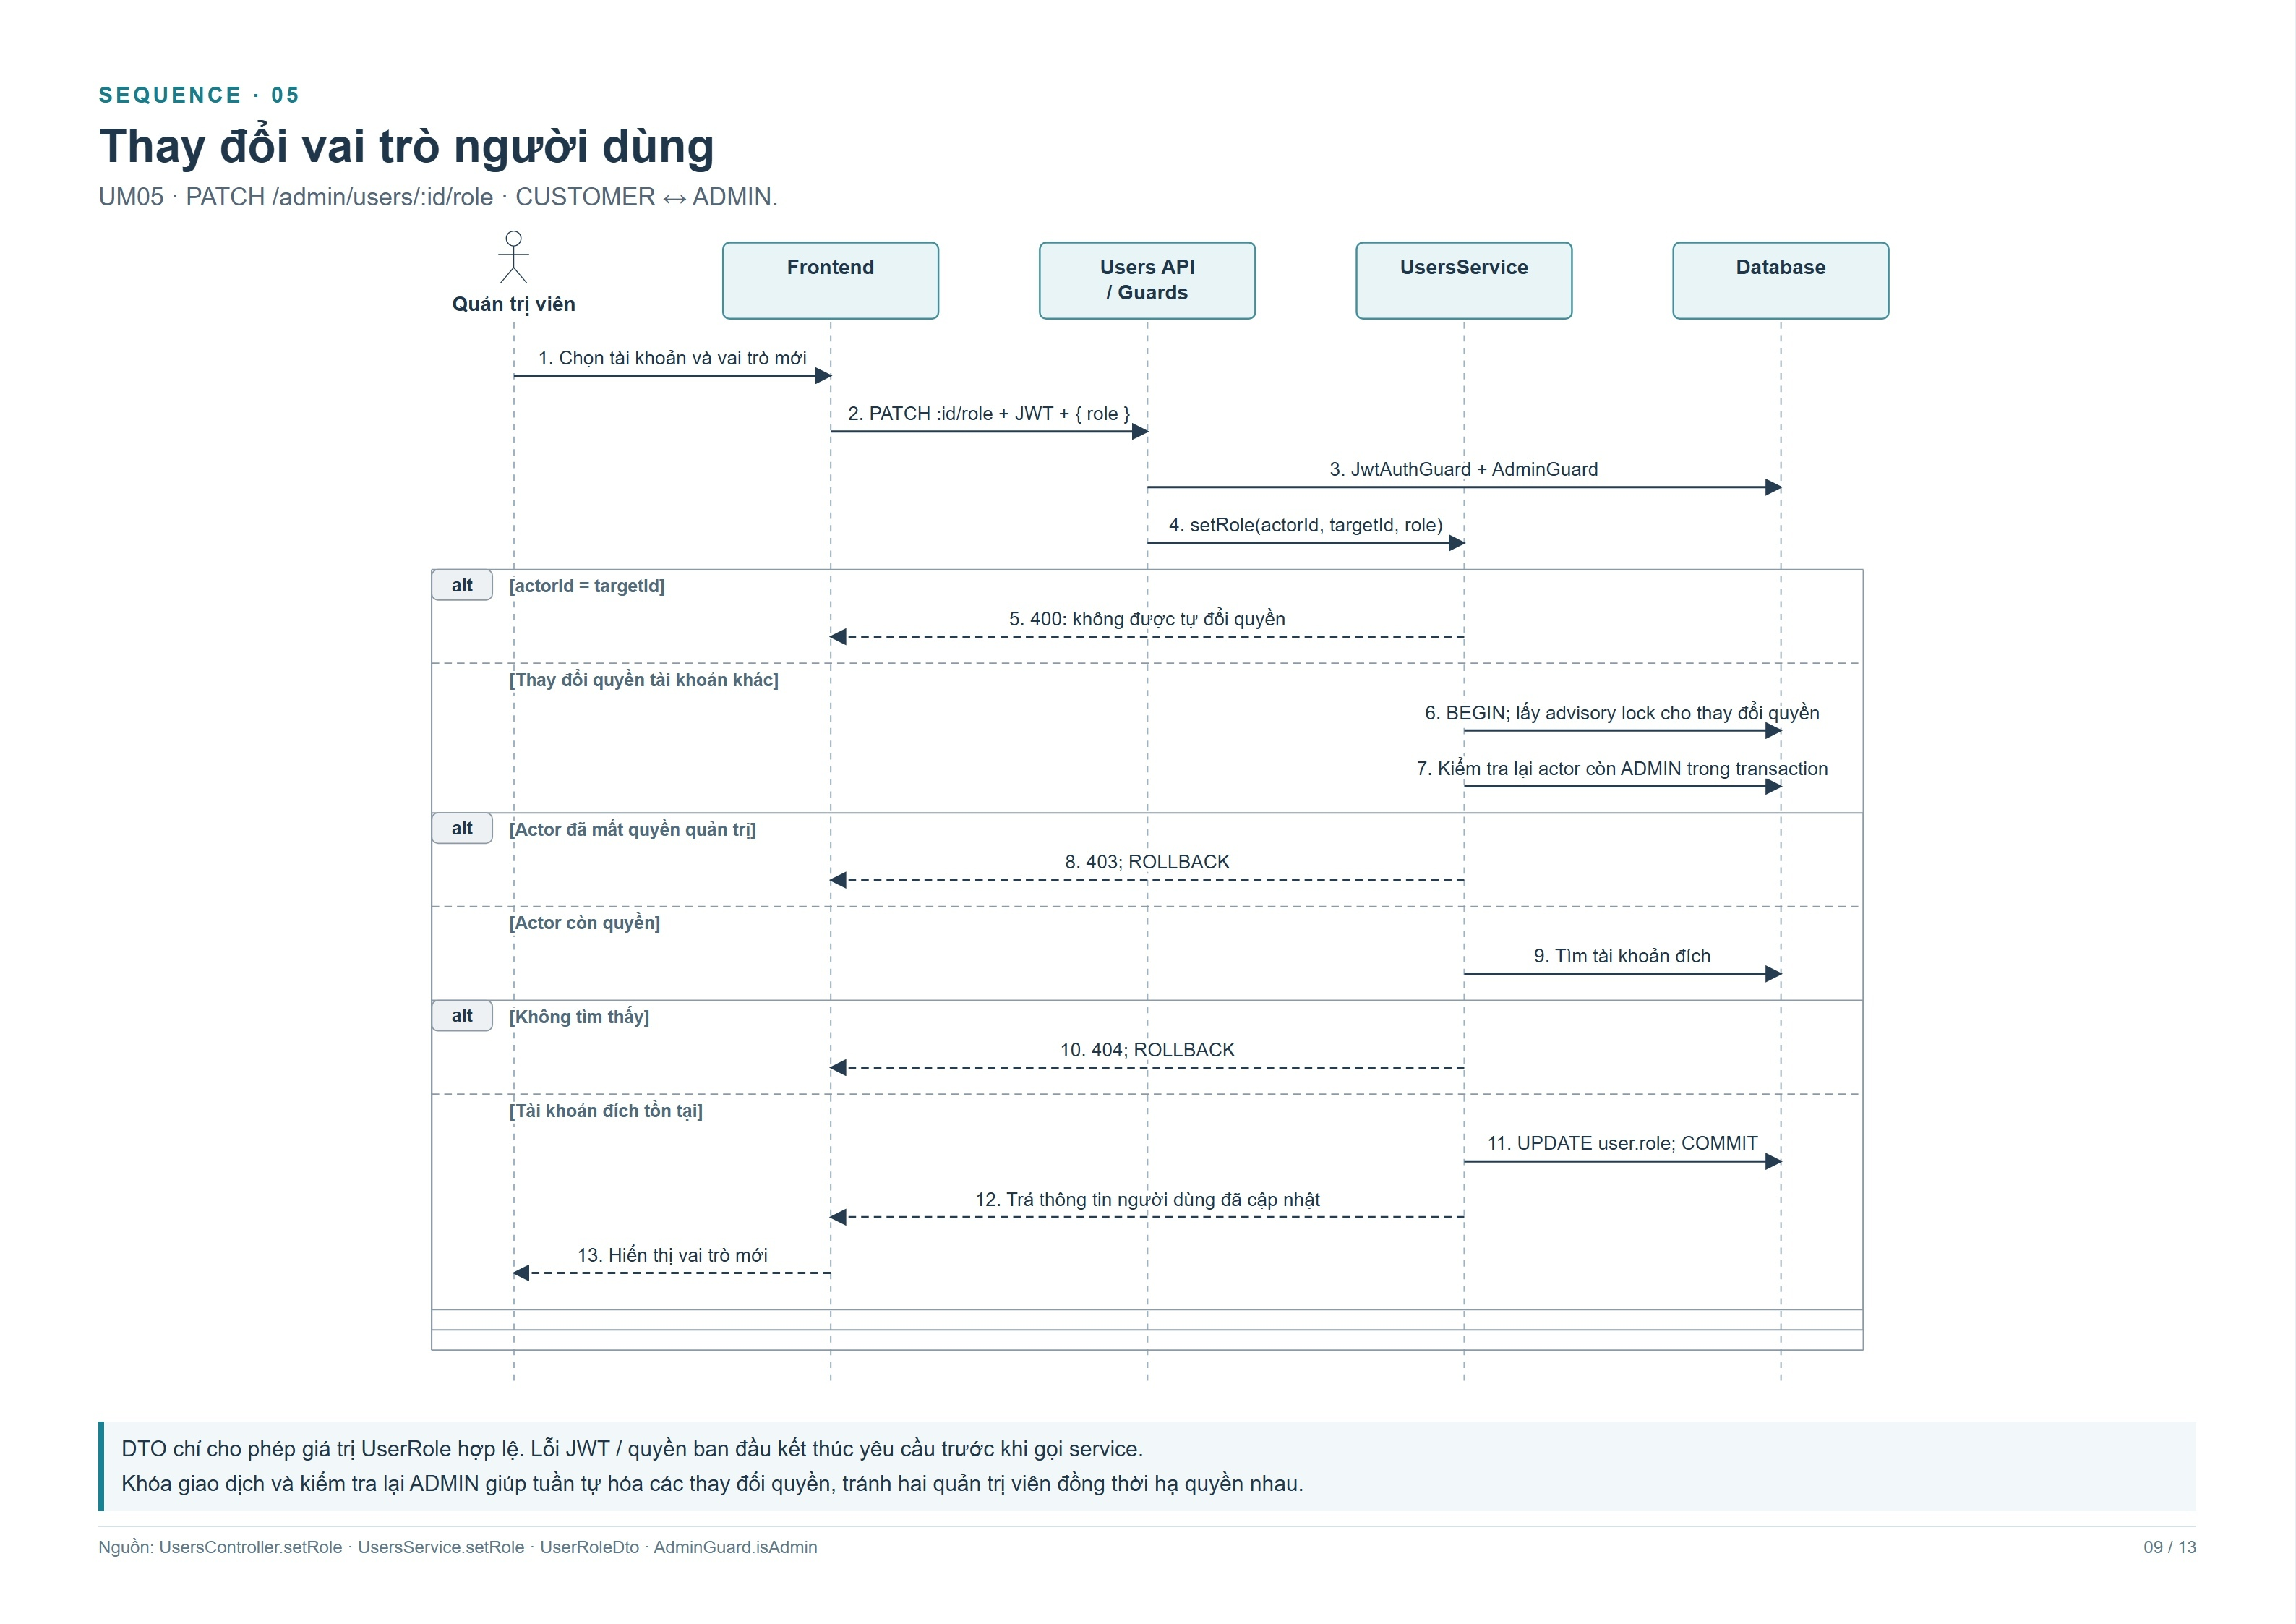
\includegraphics[width=\textwidth,height=0.48\textheight,keepaspectratio]{../figures/diagrams/sd-user-change-role-hd.png}
\caption{Sequence Diagram: Thay đổi vai trò người dùng (UM05)}
\label{fig:sd-user-change-role}
\end{figure}

% =====================================================================
%  Phụ lục H: Phân hệ Quản lý công thức định lượng (Recipe Management)
%  Nguồn: backend/src/modules/recipes/*
% =====================================================================
\section{Phân hệ Quản lý định lượng và công thức pha chế (Recipe Management Module)}
\label{app:recipe-mgmt}

Phân hệ quản lý cấu trúc công thức pha chế (Bill of Materials -- BOM) theo từng kích cỡ món uống, quản lý danh mục nguyên liệu và kiểm soát toàn vẹn dữ liệu tồn kho.

\subsection{Sơ đồ Use Case: Quản lý định lượng và công thức}

\begin{figure}[H]
\centering
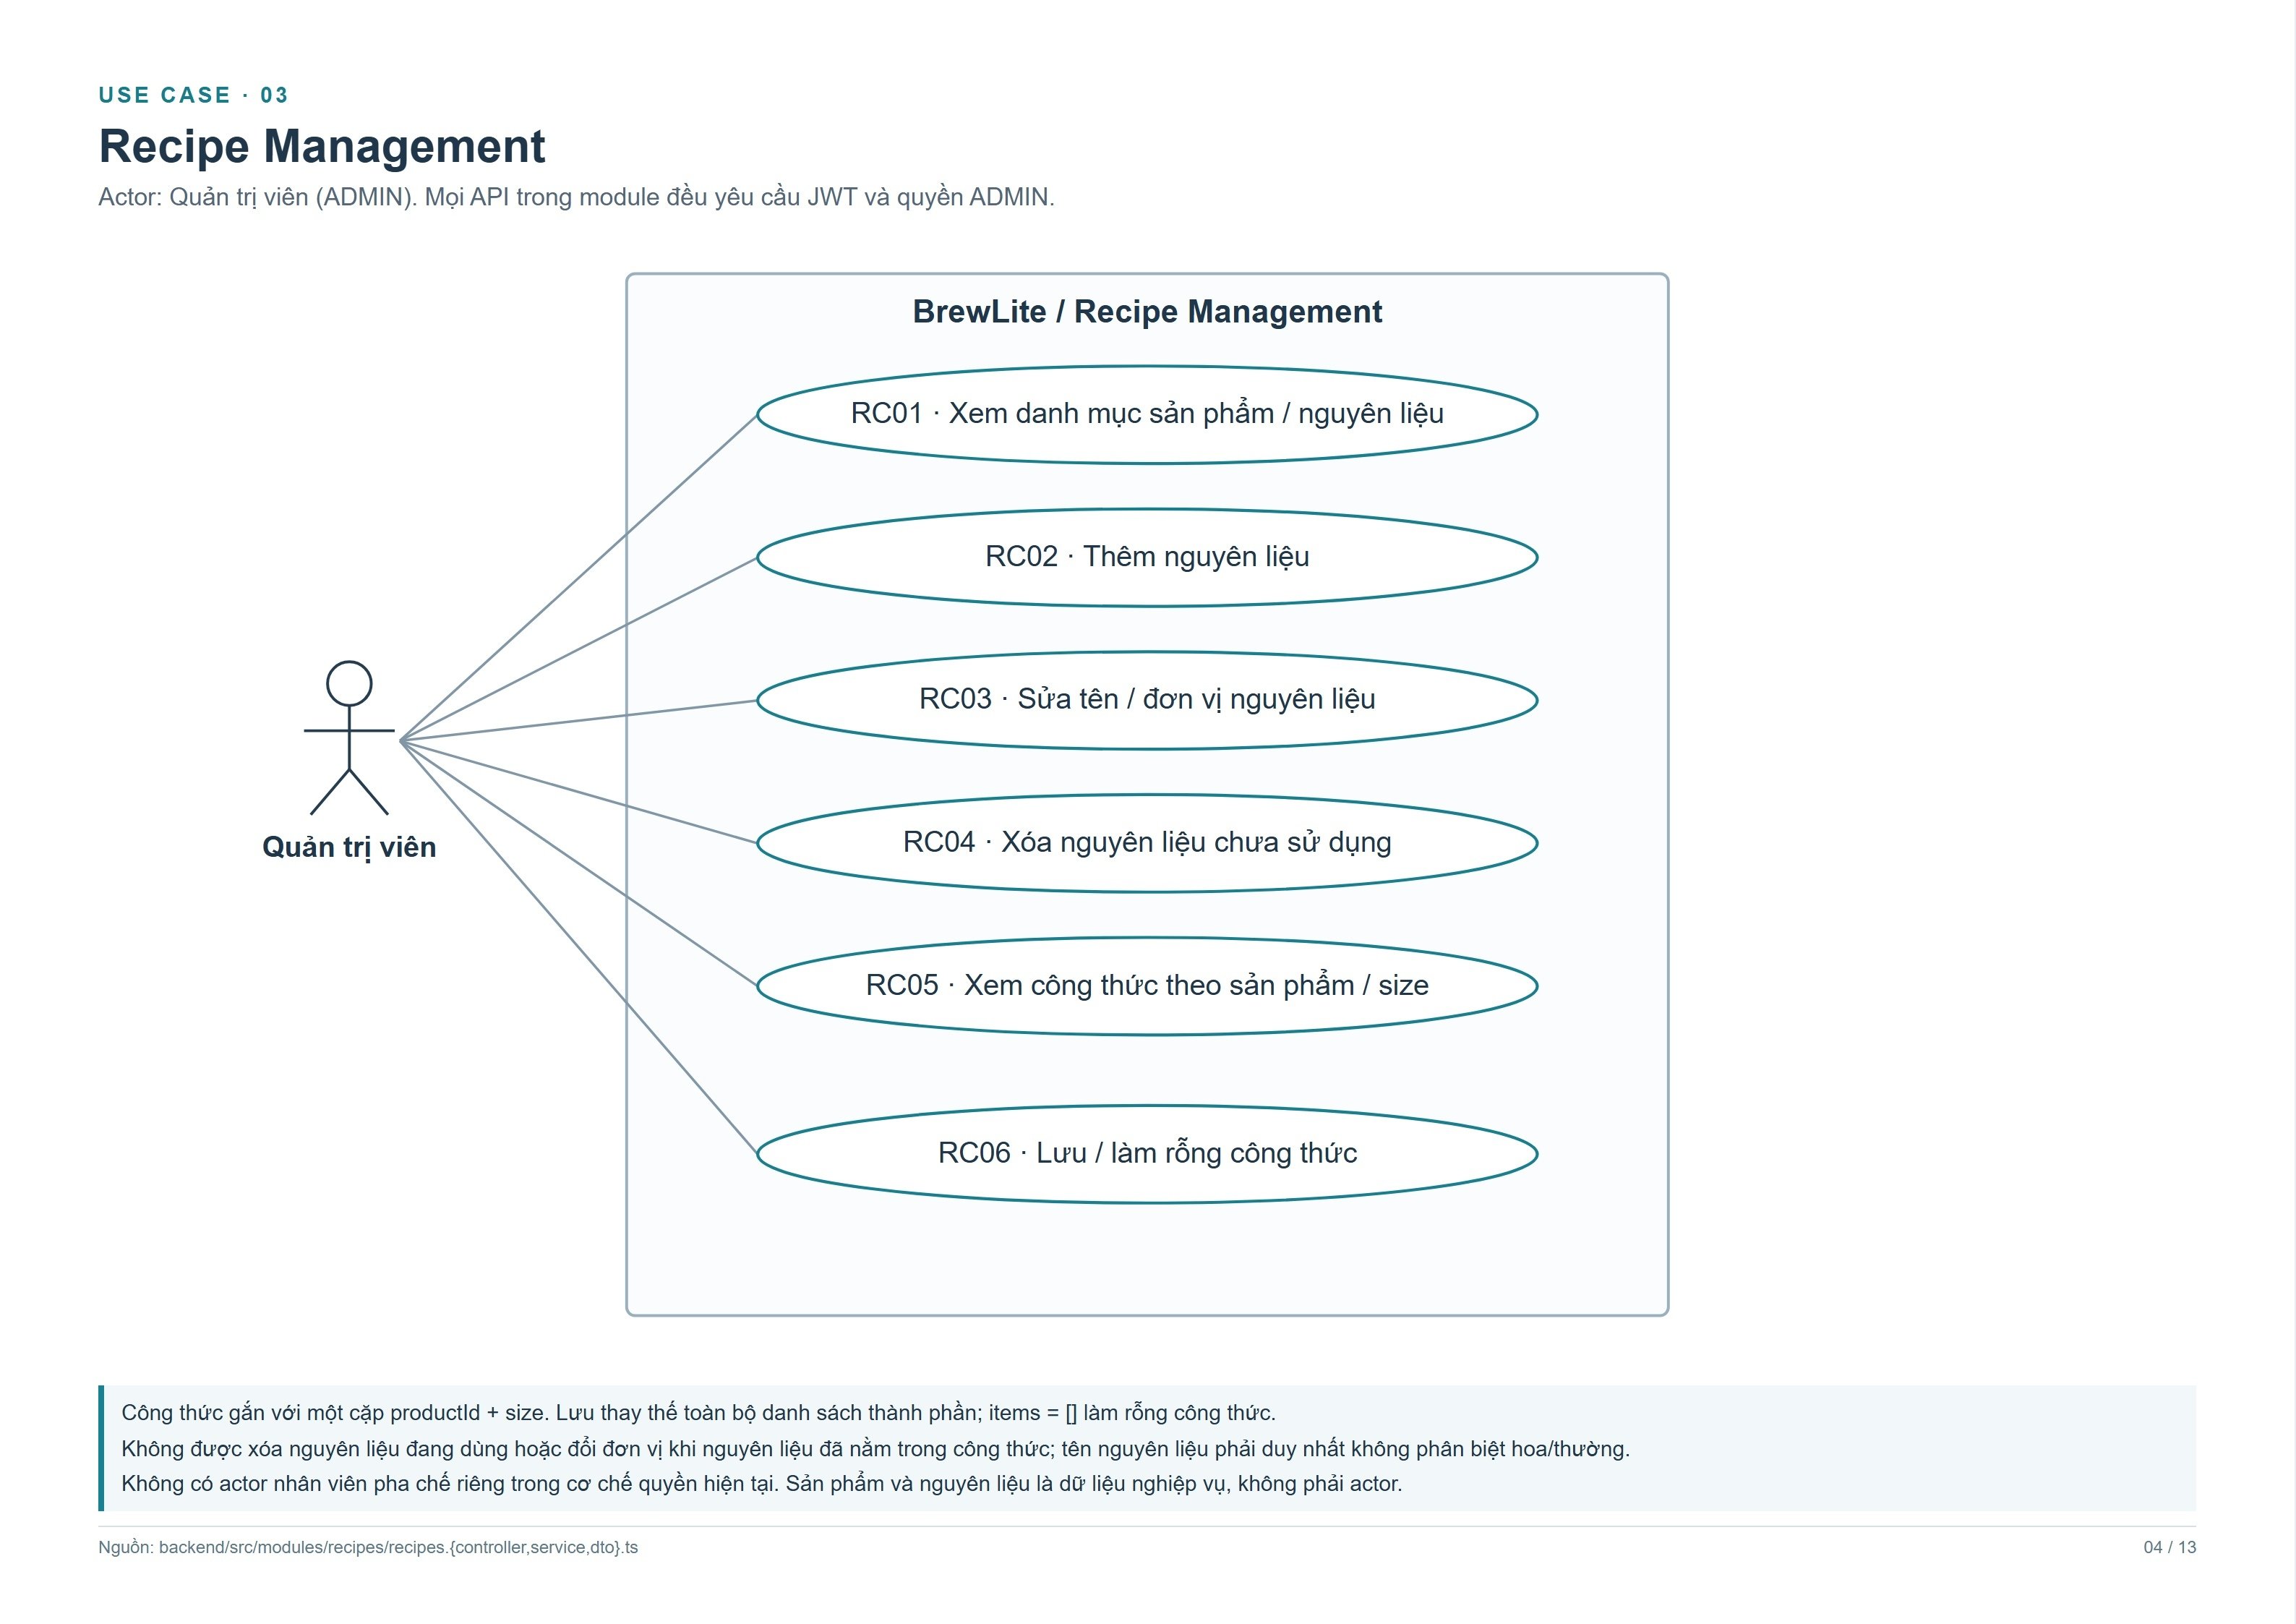
\includegraphics[width=\textwidth,height=0.45\textheight,keepaspectratio]{../figures/diagrams/uc-recipe-mgmt-hd.png}
\caption{Use Case Diagram: Phân hệ Quản lý công thức pha chế (RC01 -- RC06)}
\label{fig:uc-recipe-mgmt}
\end{figure}

\begin{table}[H]
\centering\small
\caption{Danh mục Use Case phân hệ Quản lý công thức pha chế}
\label{tab:uc-recipe-list}
\begin{tabularx}{\textwidth}{@{}l p{4.5cm} X p{3.2cm}@{}}
\toprule
\textbf{Mã UC} & \textbf{Tên Use Case} & \textbf{Mô tả nghiệp vụ} & \textbf{Endpoint / Guard} \\
\midrule
RC01 & Xem danh mục sản phẩm / nguyên liệu & Xem tổng hợp các mặt hàng kèm số lượng thành phần công thức đang có. & \code{GET /admin/recipes/catalog} \\
RC02 & Thêm nguyên liệu & Đăng ký nguyên liệu mới vào hệ thống kèm đơn vị tính chuẩn hóa. & \code{POST /admin/recipes/ingredients} \\
RC03 & Sửa tên / đơn vị nguyên liệu & Cập nhật tên gọi hoặc đơn vị tính cho nguyên liệu đã tạo. & \code{PATCH /admin/recipes/ingredients/:id} \\
RC04 & Xóa nguyên liệu chưa sử dụng & Xóa bỏ nguyên liệu khỏi hệ thống khi chưa từng gắn vào bất kỳ công thức nào. & \code{DELETE /admin/recipes/ingredients/:id} \\
RC05 & Xem công thức theo sản phẩm / size & Xem bảng định lượng chi tiết các thành phần cho một kích cỡ cụ thể của món. & \code{GET /admin/recipes/:productId/:size} \\
RC06 & Lưu / làm rỗng công thức & Thiết lập mới, thay thế hoặc xóa trắng toàn bộ định lượng của một cặp sản phẩm/size. & \code{PUT /admin/recipes/:productId/:size} \\
\bottomrule
\end{tabularx}
\end{table}

\begin{note}[Quy tắc bảo vệ toàn vẹn dữ liệu định lượng BOM]
\begin{enumerate}[label=\alph*.]
  \item \textbf{Cấm xóa nguyên liệu đang dùng:} Nếu nguyên liệu đã được liên kết trong bất kỳ công thức nào (\code{recipeCount > 0}), API từ chối xóa và trả lỗi \code{409 Conflict}. Không cho phép cascade xóa tự động để bảo vệ lịch sử đơn hàng.
  \item \textbf{Cấm đổi đơn vị tính khi đã có trong công thức:} Đổi đơn vị tính của nguyên liệu đang dùng sẽ làm sai lệch hoàn toàn phép tính trừ kho khi đặt hàng; do đó thao tác này bị chặn với mã lỗi \code{409 Conflict}.
  \item \textbf{Lưu công thức nguyên tử (Atomic BOM Replacement):} Khi lưu công thức, hệ thống sử dụng khóa \code{FOR SHARE} trên các nguyên liệu thành phần và \code{FOR UPDATE} trên bản ghi giá kích cỡ, xóa các dòng cũ và chèn toàn bộ dòng mới trong cùng một transaction. Dữ liệu rỗng \code{items = []} mang ý nghĩa làm rỗng công thức hợp lệ.
\end{enumerate}
\end{note}

\subsection{Các sơ đồ tuần tự chi tiết của phân hệ Công thức pha chế}

\subsubsection{Sequence: Xem danh mục và công thức theo kích cỡ (RC01, RC05)}
\begin{figure}[H]
\centering
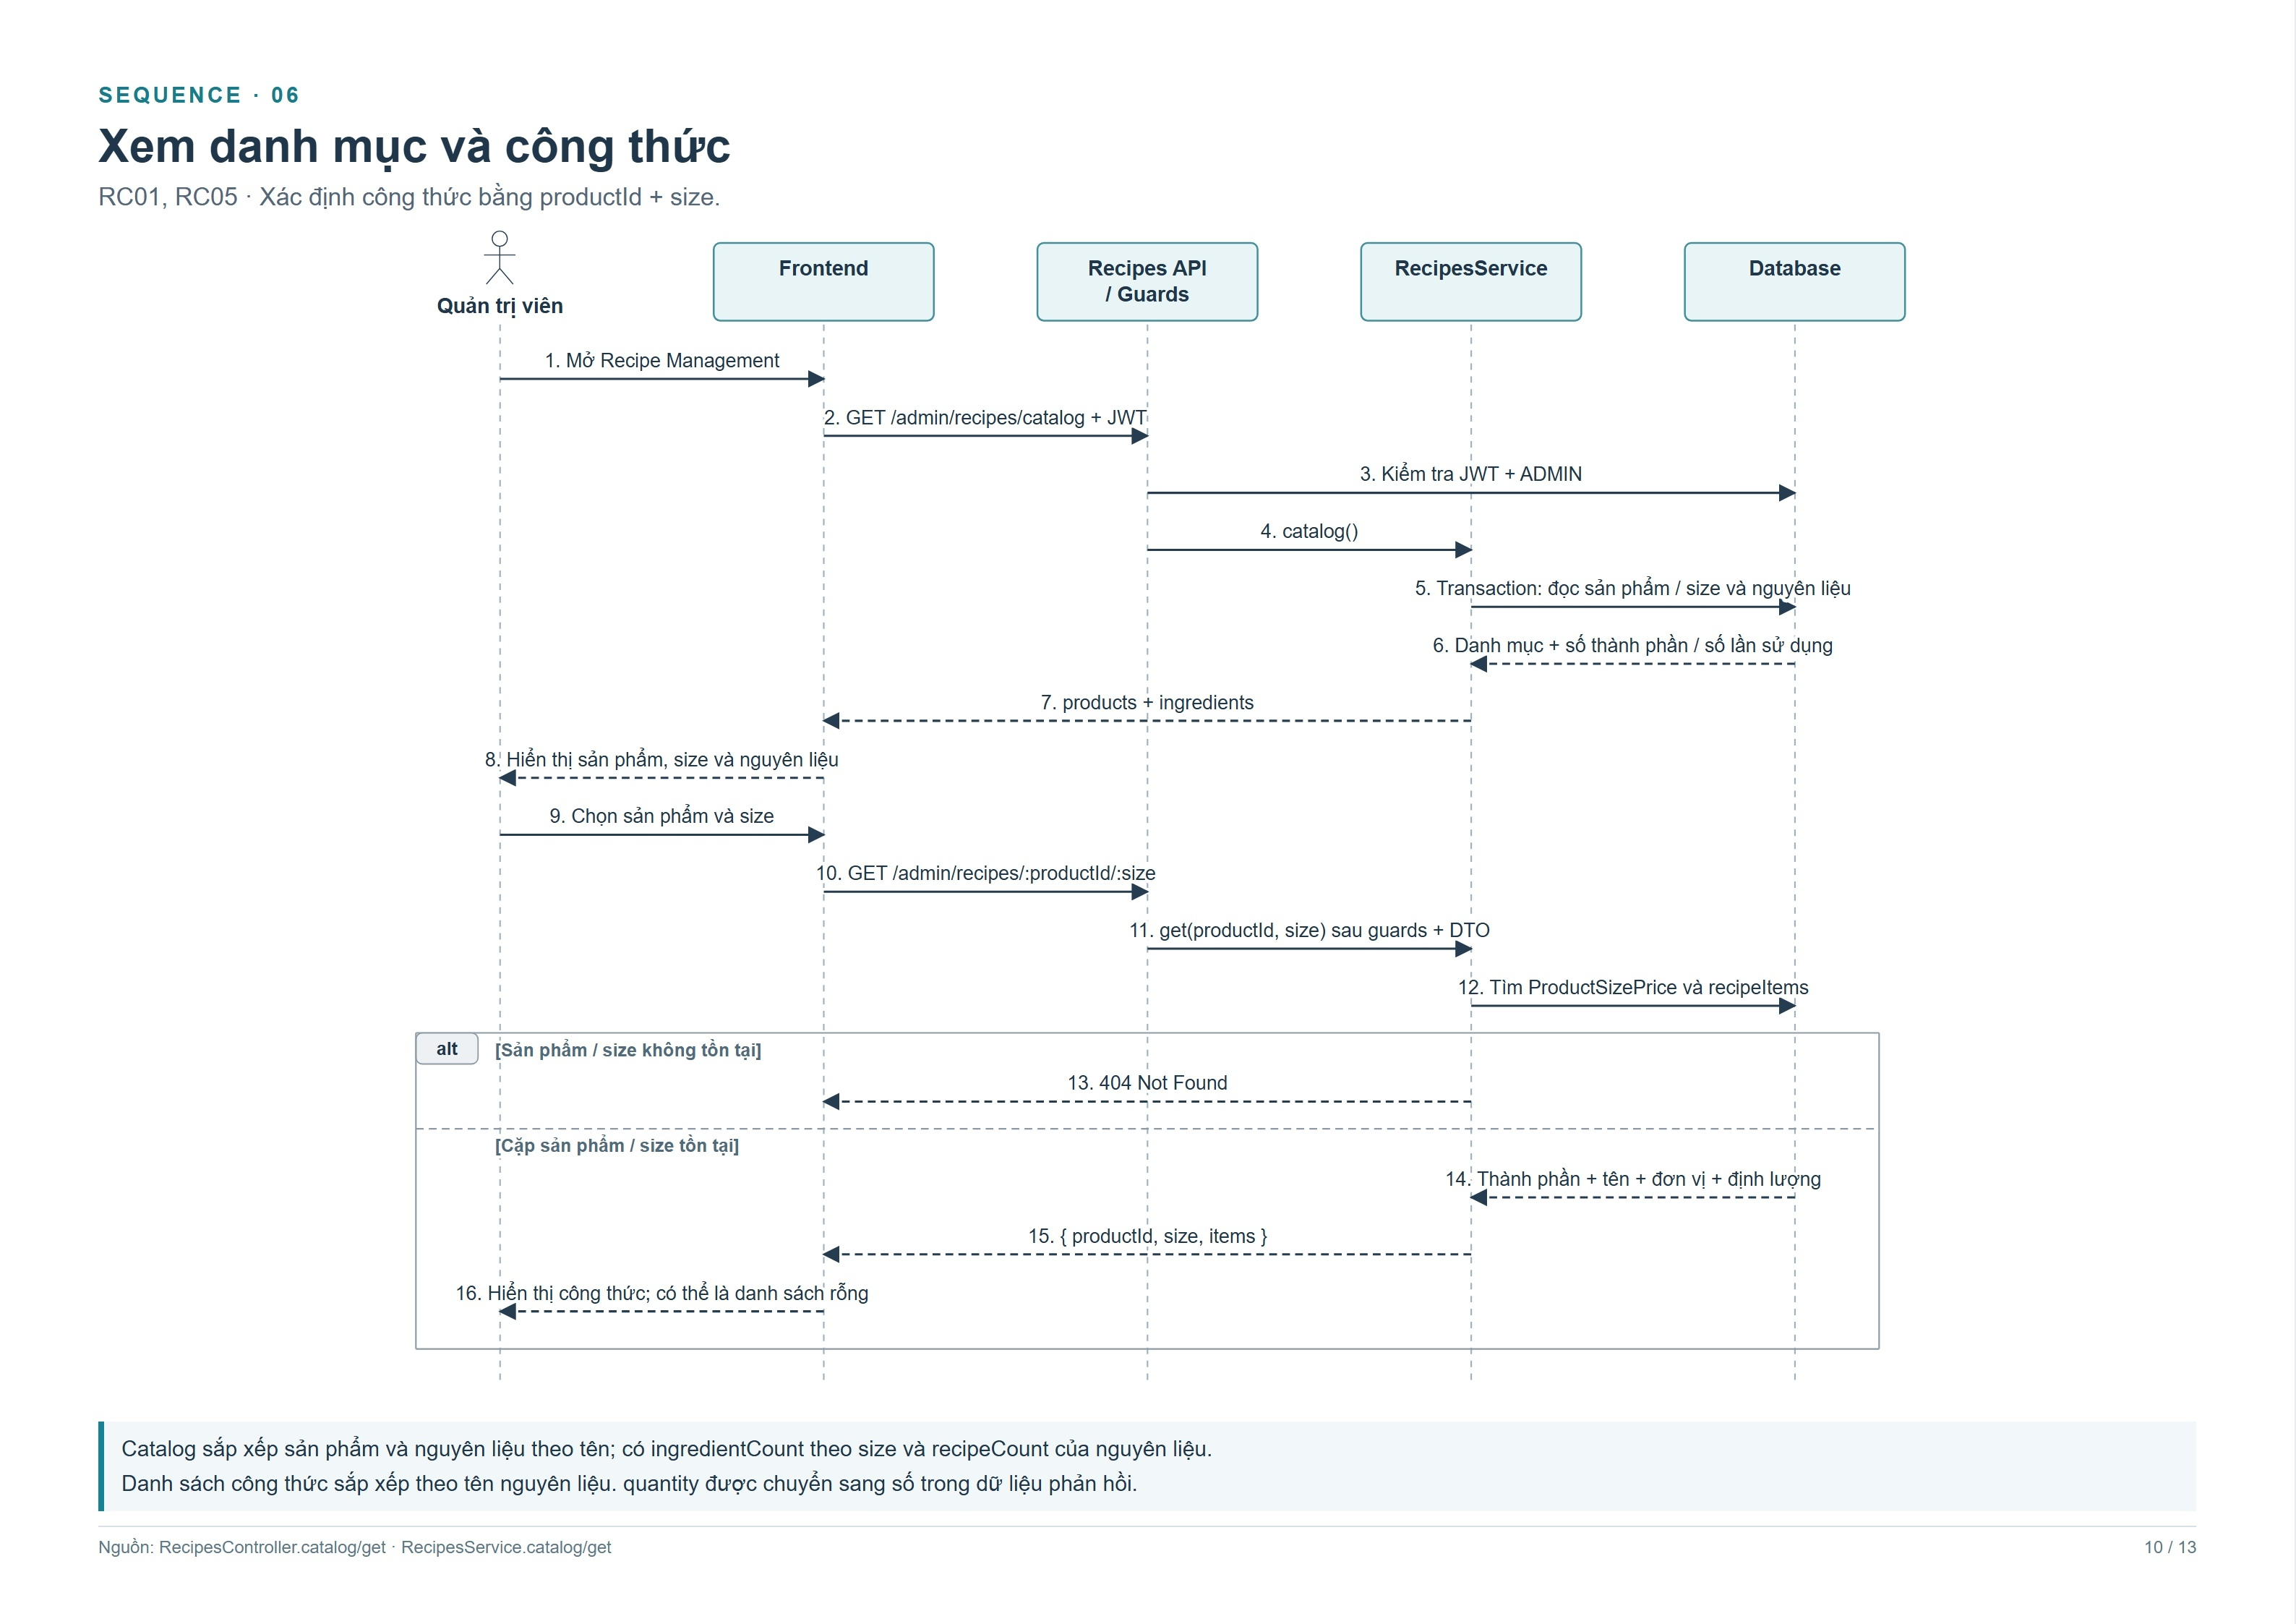
\includegraphics[width=\textwidth,height=0.48\textheight,keepaspectratio]{../figures/diagrams/sd-recipe-catalog-hd.png}
\caption{Sequence Diagram: Xem danh mục và chi tiết công thức (RC01, RC05)}
\label{fig:sd-recipe-catalog}
\end{figure}

\subsubsection{Sequence: Thêm và sửa nguyên liệu (RC02, RC03)}
\begin{figure}[H]
\centering
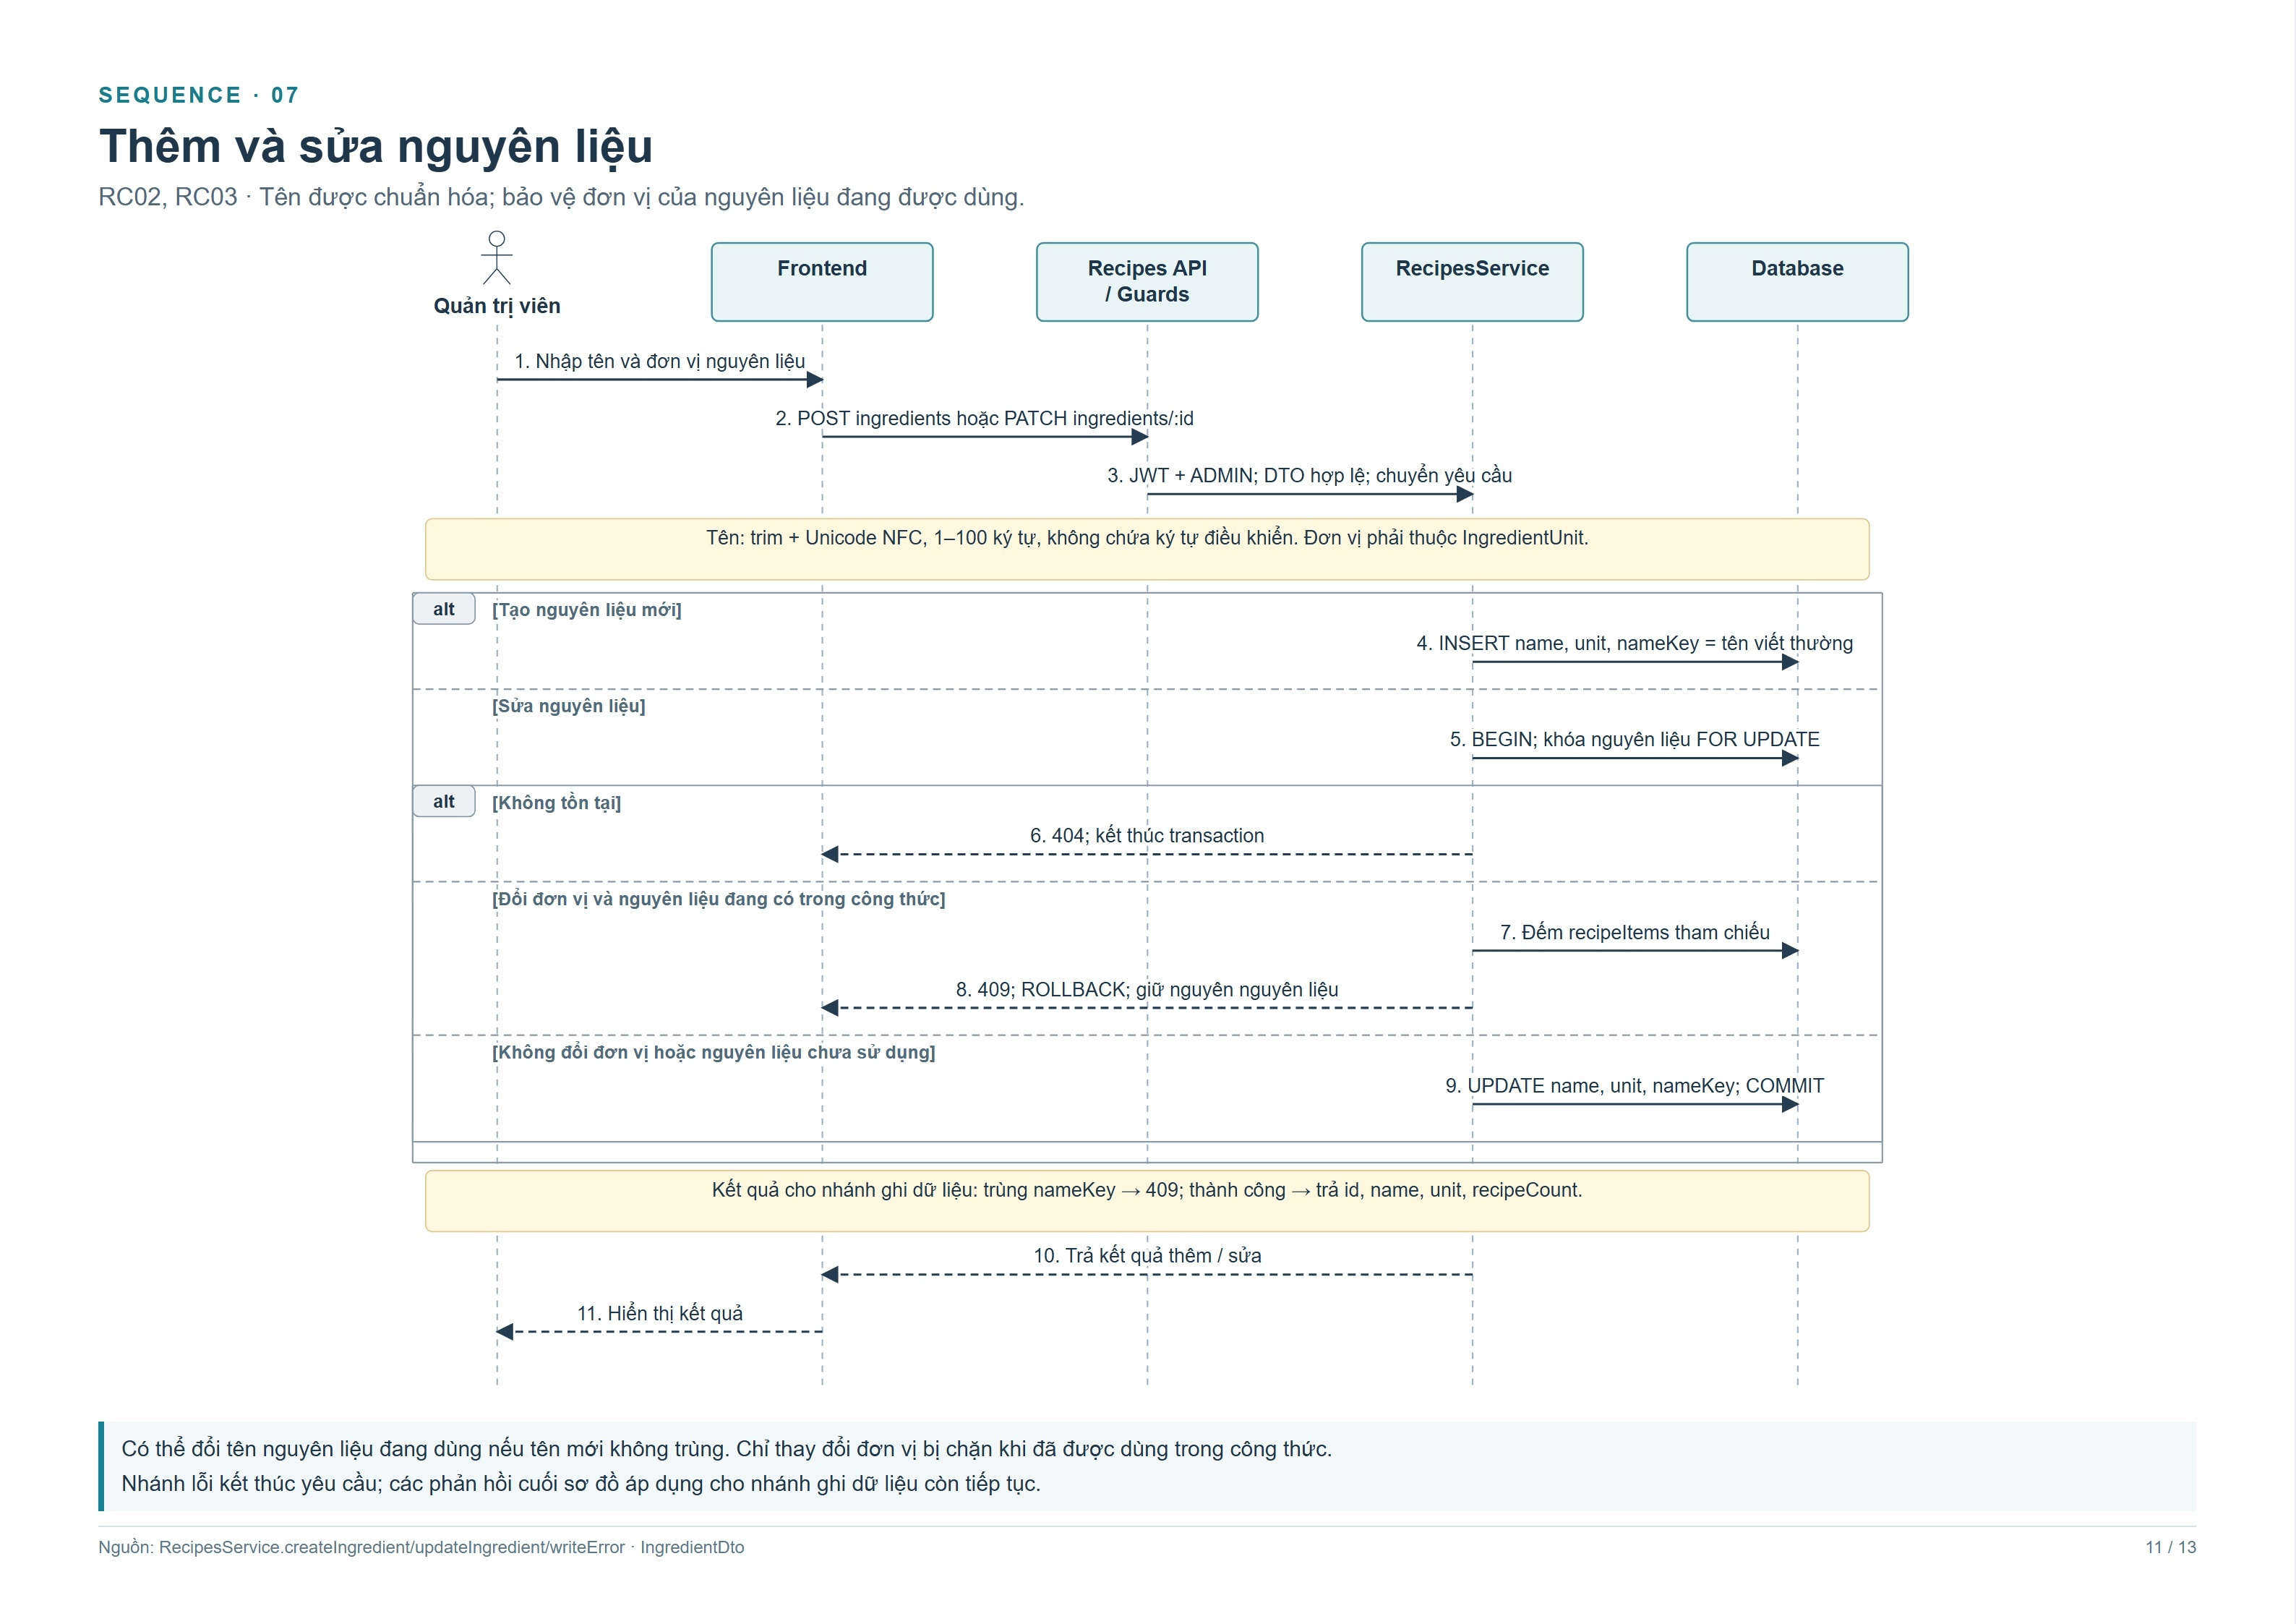
\includegraphics[width=\textwidth,height=0.48\textheight,keepaspectratio]{../figures/diagrams/sd-recipe-ingredient-add-edit-hd.png}
\caption{Sequence Diagram: Thêm và sửa nguyên liệu (RC02, RC03)}
\label{fig:sd-recipe-ingredient-add-edit}
\end{figure}

\subsubsection{Sequence: Xóa nguyên liệu chưa sử dụng (RC04)}
\begin{figure}[H]
\centering
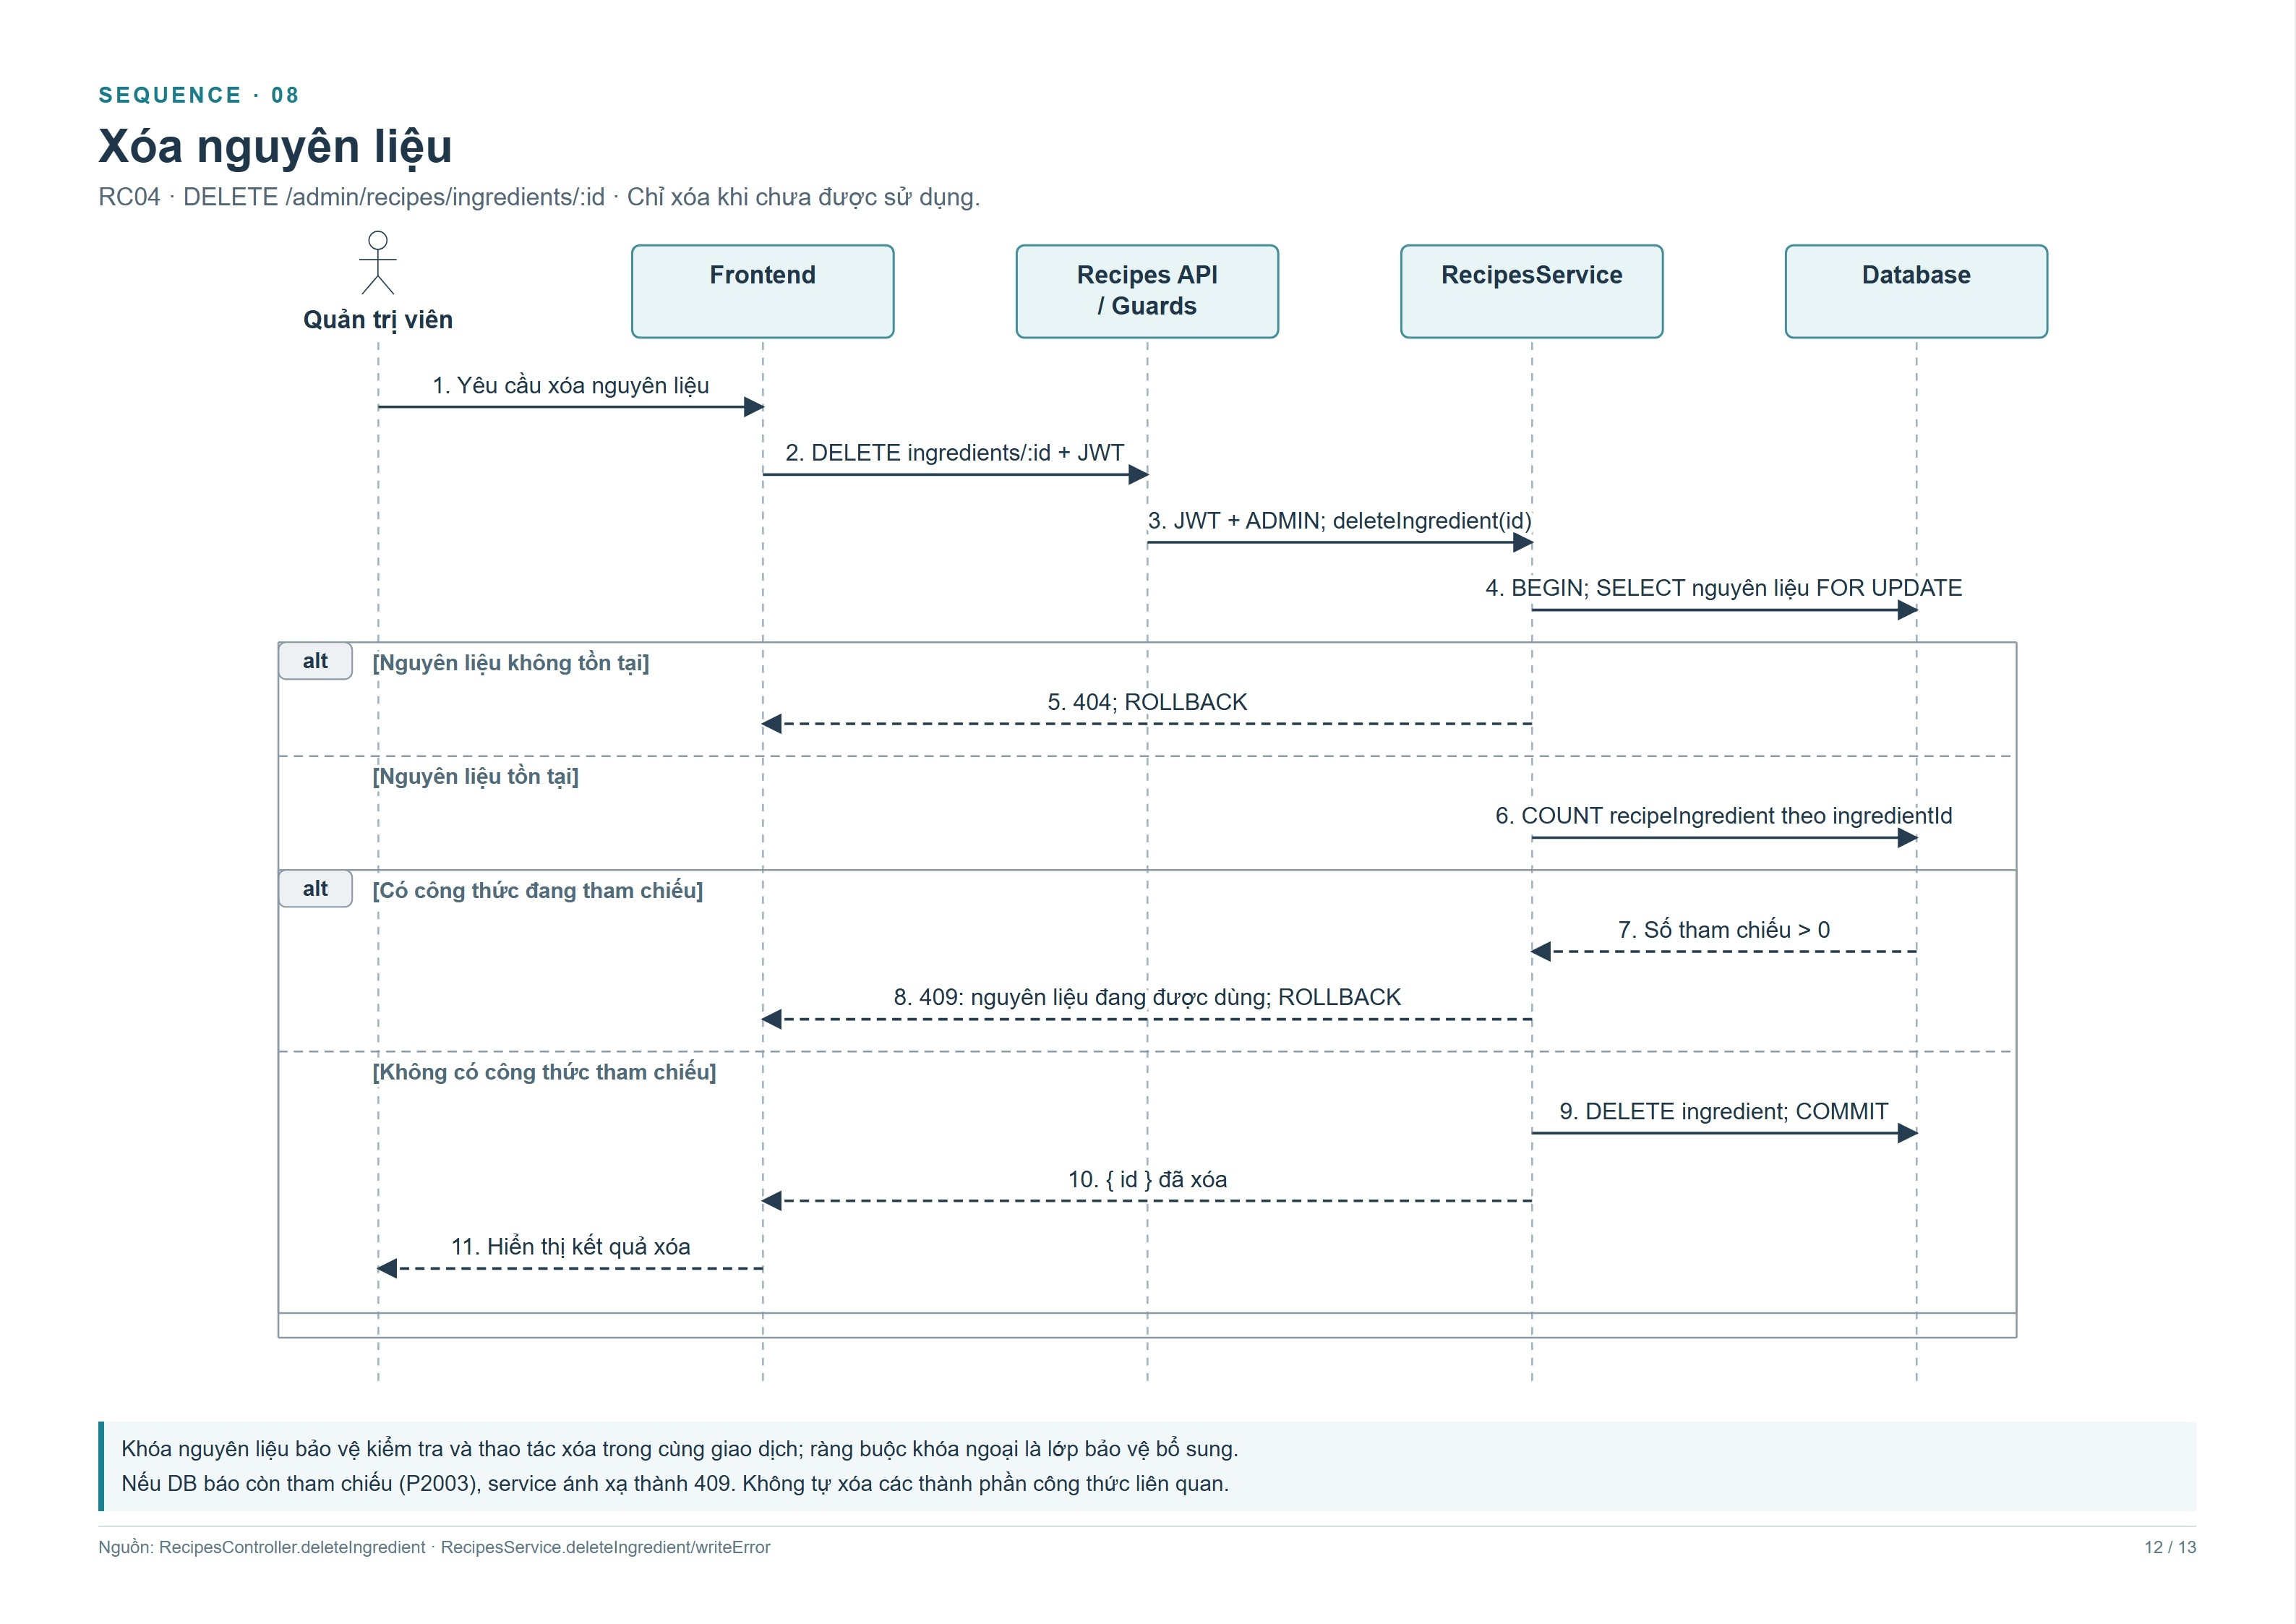
\includegraphics[width=\textwidth,height=0.48\textheight,keepaspectratio]{../figures/diagrams/sd-recipe-ingredient-delete-hd.png}
\caption{Sequence Diagram: Xóa nguyên liệu chưa sử dụng (RC04)}
\label{fig:sd-recipe-ingredient-delete}
\end{figure}

\subsubsection{Sequence: Lưu hoặc làm rỗng công thức pha chế (RC06)}
\begin{figure}[H]
\centering
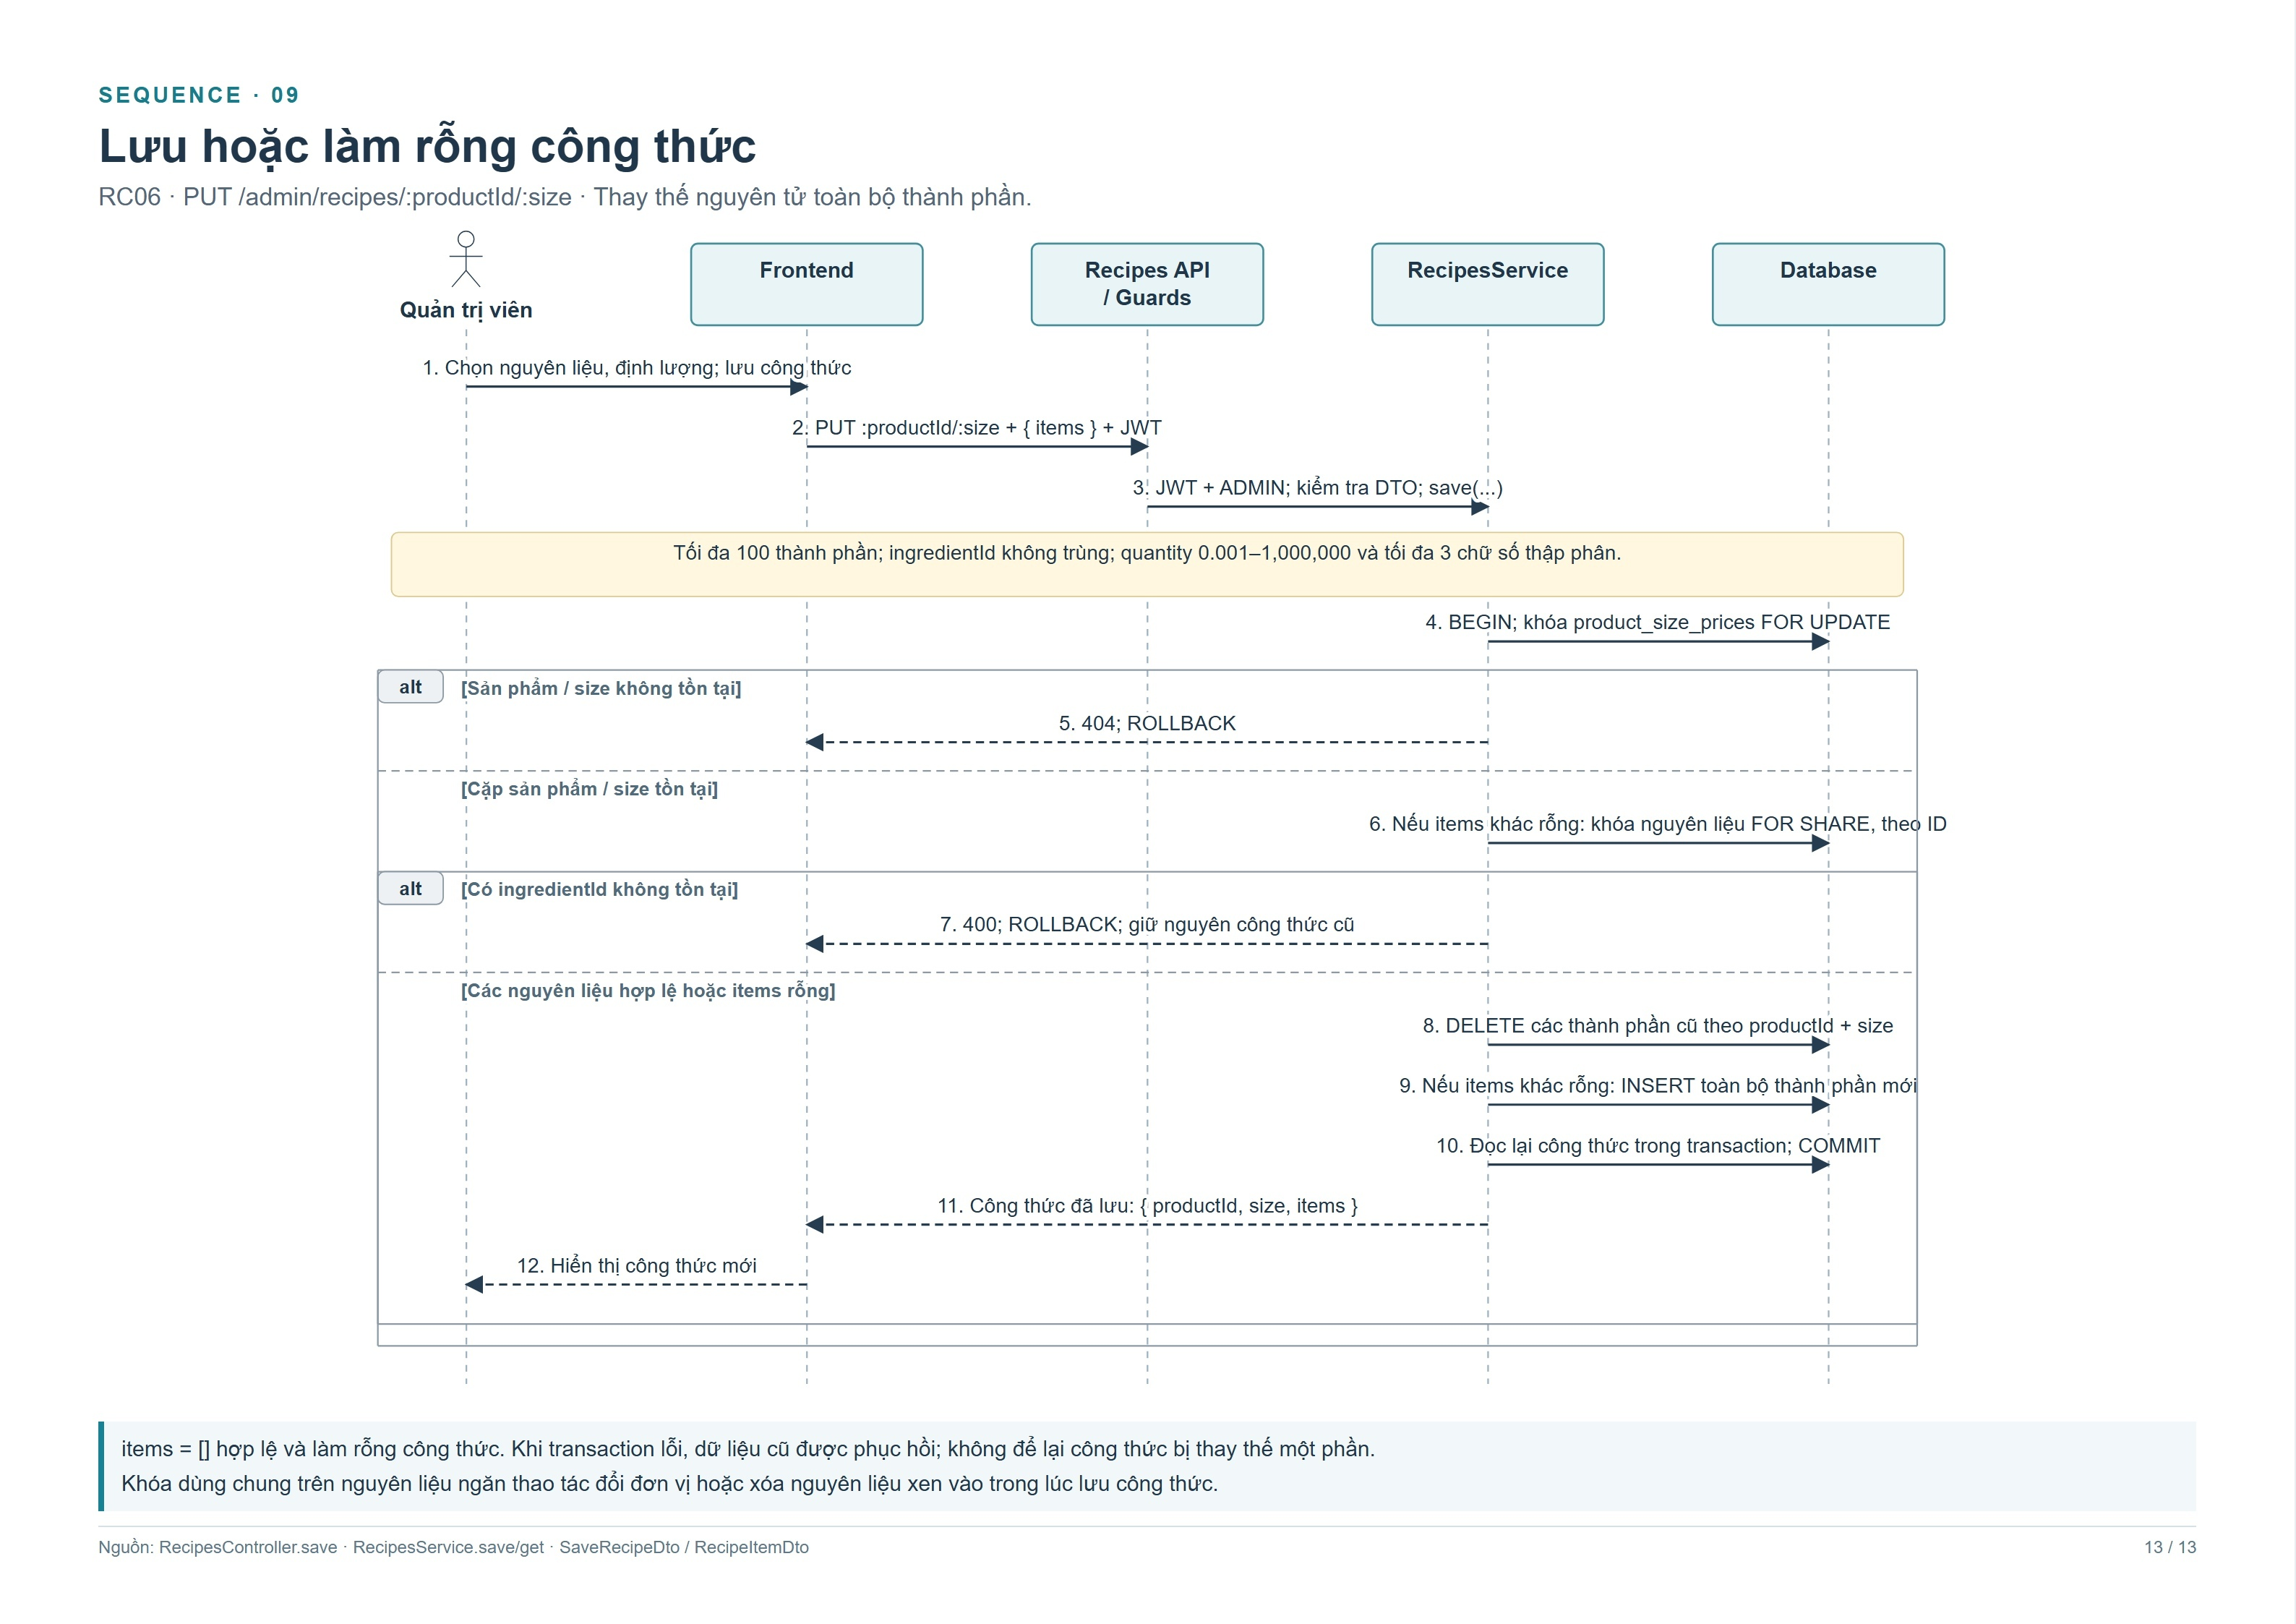
\includegraphics[width=\textwidth,height=0.48\textheight,keepaspectratio]{../figures/diagrams/sd-recipe-save-hd.png}
\caption{Sequence Diagram: Lưu hoặc làm rỗng công thức (RC06)}
\label{fig:sd-recipe-save}
\end{figure}
